% Do not change document class, margins, fonts, etc.
\documentclass[a4paper,oneside,bibliography=totoc]{scrbook}

% some useful packages (add more as needed)
\usepackage{scrhack}
\usepackage[utf8]{inputenc}
\usepackage{graphicx}
\usepackage{latexsym}
\usepackage{amsmath}
\usepackage{amssymb}
\usepackage{tabularx}
\usepackage{csquotes}
\usepackage{booktabs}
\usepackage{listings}
\usepackage{algorithm}
\counterwithin{algorithm}{chapter}
\usepackage{algorithmic}
\usepackage{csquotes}
\renewcommand{\algorithmiccomment}[1]{\hfill\textit{// #1}}
\usepackage[usenames,dvipsnames]{xcolor}
\usepackage[colorlinks,citecolor=Green]{hyperref}
\usepackage{lipsum}
\usepackage[printonlyused]{acronym}

% chicago citation style
\usepackage{natbib}
\bibliographystyle{chicagoa}
\setcitestyle{authoryear,round,semicolon,aysep={},yysep={,}} \let\cite\citep

% example enviroments (add more as needed)
\newtheorem{definition}{Definition} \newtheorem{proposition}{Proposition}

% Definition einer Turtle-Sprache
\lstdefinelanguage{Turtle}{
  morekeywords={@prefix,@base,a},
  morekeywords=[2]{ex,exp,rdfs},
  morestring=[b]",
  morestring=[b]',
  sensitive=true,
  basicstyle=\small\ttfamily,
  keywordstyle=\color{blue},
  keywordstyle=[2]\color{magenta},
  commentstyle=\color{gray}\itshape,
  stringstyle=\color{OliveGreen},
  columns=fullflexible,
  breaklines=true,
  breakatwhitespace=false,
  literate={:}{{{\color{orange}:}}}1,
}

% Definition einer SPARQL-Sprache
\lstdefinelanguage{SPARQL}{
  morekeywords={@prefix,@base,a,SELECT,WHERE},
  morekeywords=[2]{ex,exp,rdfs},
  morestring=[b]",
  morestring=[b]',
  sensitive=true,
  basicstyle=\small\ttfamily,
  keywordstyle=\color{blue},
  keywordstyle=[2]\color{magenta},
  commentstyle=\color{gray}\itshape,
  stringstyle=\color{OliveGreen},
  columns=fullflexible,
  breaklines=true,
  breakatwhitespace=false,
  literate={:}{{{\color{orange}:}}}1,
}

% Globales Styling für alle Listings
\lstset{
  language=Turtle,
  frame=single,
  numbers=left,
  numberstyle=\tiny\color{gray},
  numbersep=5pt,
  tabsize=2,
  captionpos=b,
  basicstyle=\small\ttfamily,
}

\begin{document}

\frontmatter
\subject{Master Thesis}
\title{CIExMAS: Closed Information Extraction using a Multi-Agent-System}
\author{Max Lautenbach\\
  (matriculation number 1980683)}
\date{18.08.2025}
\publishers{{\small Submitted to}\\
  Data and Web Science Group\\
  Dr.\ Sven Hertling\\
  University of Mannheim\\}
\maketitle

\chapter{Abstract}

Closed information extraction has so far relied mainly on fine-tuned transformer models that require large training datasets. However, advances in large language models and agent-based artificial intelligence have not yet been explored in this context. In this work, we introduce CIExMAS, a collection of modular architectures based on multi-agent systems for closed information extraction without the need for fine-tuning. The best architecture comprises specialized agents for triple extraction, uniform resource identifier mapping, and validation, supported by tools for integration with knowledge graphs. CIExMAS is designed as an exploratory framework that tests a broad range of architectural setups to evaluate the general feasibility of multi-agent systems in this domain. In our evaluation, CIExMAS achieved up to 80\% of the performance of current state-of-the-art models—despite requiring no supervised training. This result highlights the effectiveness of agent-based approaches in closed information extraction and points to their potential as flexible, scalable, and lightweight alternatives. As an initial study in this direction, CIExMAS lays the foundation for further research at the intersection of agent-based artificial intelligence and closed information extraction.

\begingroup%
\hypersetup{hidelinks}%
\tableofcontents%
\endgroup

\begingroup%
\hypersetup{hidelinks}%
\listoffigures%
\addcontentsline{toc}{chapter}{List of Figures}
\endgroup

\begingroup%
\hypersetup{hidelinks}%
\listoftables%
\addcontentsline{toc}{chapter}{List of Tables}
\endgroup

\chapter{List of Abbreviations}
\begin{acronym}
  \acro{AI}{Artificial Intelligence}
  \acro{CoT}{Chain of Thought}
  \acro{CRM}{Customer Relationship Management}
  \acro{DBMS}{Database Management System}
  \acro{GPT}{Generative Pre-trained Transformer}
  \acro{ICL}{In-Context Learning}
  \acro{IE}{Information Extraction}
  \acro{KG}{Knowledge Graph}
  \acro{LLM}{Large Language Model}
  \acro{LLaMA}{Large Language Model Meta AI}
  \acro{LM}{Language Model}
  \acro{MAS}{Multi-Agent System}
  \acro{ML}{Machine Learning}
  \acro{NLP}{Natural Language Processing}
  \acro{OWL}{Web Ontology Language}
  \acro{RAG}{Retrieval Augmented Generation}
  \acro{RDF}{Resource Description Framework}
  \acro{RDFS}{Resource Description Framework Schema}
  \acro{SPARQL}{SPARQL Protocol and RDF Query Language}
  \acro{SSA}{Splitted Supervisor Architecture}
  \acro{SSSA}{Simplified Splitted Supervisor Architecture}
  \acro{URI}{Uniform Resource Identifier}
  \acro{VDBMS}{Vector Database Management System}
  \acro{cIE}{Closed Information Extraction}

\end{acronym}

\mainmatter

\chapter{Introduction}
\label{ch:introduction}

\acp{LM}, and especially modern \acp{LLM}, have significantly improved the ability of machines to understand and generate human language. These models have enabled progress in various downstream tasks ranging from question answering to summarization and reasoning \cite{Brown2020}. However, their static training data limits their ability to incorporate new or domain-specific knowledge — a limitation known as the knowledge cutoff problem. Most \acp{LLM} are trained once on large corpora and as a result, they have no built-in access to information that emerged after the end of their training period and cannot retrieve up-to-date or external knowledge out of the box \cite{Brown2020,Grattafiori2024}.

As a result, there is a growing interest in structured external knowledge sources, especially \acp{KG}, to provide reliable and semantically rich context for generative models \cite{Korolov2025}. \acp{KG} allow information to be represented in a formal, machine-interpretable way, which makes them highly suitable for integration into retrieval-augmented generation systems, question answering pipelines, and reasoning engines \cite{Korolov2025,Paulheim2016}. The increasing use of \ac{LLM}-based applications has therefore renewed attention on \acp{KG} as critical infrastructure for trustworthy and explainable \ac{AI} \cite{Korolov2025}.

At the same time, this demand creates a practical challenge: many enterprise or domain-specific knowledge graphs do not yet exist in structured form. Most relevant knowledge is still locked in unstructured text documents, reports, or communication logs \cite{Korolov2025}. To make this information accessible to downstream applications, it must be transformed into structured representations — ideally in a way that aligns with a predefined ontology or knowledge schema.

This transformation process leads directly to the research field of \ac{cIE}. As a specialized task within the broader area of \ac{IE}, \ac{cIE} focuses on extracting subject–predicate–object triples from text such that all components can be linked to valid entries in a target knowledge graph \cite{Josifoski2021}. This makes \ac{cIE} a crucial enabling technology for automated knowledge graph construction and maintenance.

\section{Motivation and Problem Statement}
\label{sec:motivation}

The automatic extraction of structured information from text is a long-standing goal in natural language processing. This task, generally referred to as \ac{IE}, includes subtasks such as named entity recognition, entity linking, and relation extraction. These components aim to identify real-world entities in text, assign them canonical identifiers, and detect semantic relationships between them \cite{Zhao2024}.

\ac{cIE} is a constrained subtask of \ac{IE}, where the goal is to extract subject–predicate–object triples that exactly match the identifiers and relations of a predefined \ac{KG}. In contrast to open \ac{IE} approaches, where relations may be freely expressed in natural language, \ac{cIE} requires strict alignment with the vocabulary and structure of a target ontology. This constraint makes \ac{cIE} especially relevant for applications that involve structured knowledge integration or automated \ac{KG} construction \cite{Josifoski2021}.

State-of-the-art models such as GenIE and synthIE have shown that \ac{cIE} can be performed with very high accuracy, particularly when the models are fine-tuned on a specific dataset. However, \cite{Josifoski2021,Josifoski2023} demonstrate a crucial limitation: models trained on one dataset (e.g., GenIE) do not generalize well to others (e.g., synthIE), even when the task and \ac{KG} structure remain similar. This lack of generalization highlights a key drawback of current \ac{IE} systems, which often rely on supervised fine-tuning and are closely coupled to a specific domain or knowledge graph.

This tight coupling reduces reusability and makes it difficult to adapt systems to new domains or ontologies without significant retraining. Consequently, researchers are exploring more modular alternatives that promise better generalisation without the need for task-specific fine-tuning \cite{Shi2024}.

\acp{LLM} have demonstrated strong \ac{ICL} capabilities. Rather than encoding knowledge directly into model weights, \acp{LLM} can be guided to perform tasks dynamically using prompts, examples, and external tools \cite{Brown2020}. This opens up the possibility of solving \ac{cIE} through prompting alone, without any task-specific fine-tuning.

At the same time, recent work in agentic AI explores how \acp{LLM} can be organized into multi-agent systems that interact via tool use, planning, and role-based coordination~\cite{OpenAI2025,Anthropic2024,Wiesinger2025}. These systems have shown promise for complex reasoning tasks and dynamic workflows. \citet{Shi2024} further demonstrate that even single-agent architectures can achieve state-of-the-art performance on \ac{IE} tasks.

These developments motivate the hypothesis that multi-agent systems may offer an effective and generalizable approach to \ac{cIE}. Unlike monolithic pipelines or fine-tuned models, multi-agent architectures can decompose the task into modular roles such as entity extraction, URI disambiguation, and triple validation, and combine the flexibility of prompting with external tool access. This is especially relevant when generating \ac{KG}-ready triples, as these often require lookups or validation against the underlying graph structure. Such tool use is increasingly common in modern agentic frameworks \citet{OpenAI2025} and forms the foundation of the CIExMAS architecture proposed in this thesis.

\section{Research Objectives and Questions}
\label{sec:research_questions}

This thesis investigates whether \ac{cIE} can be solved effectively by \ac{LLM}-based multi-agent systems — without relying on model fine-tuning. The central idea is to replace the monolithic, task-specific IE pipelines with distributed, role-based agents that coordinate through a shared plan or workflow. These agents can perform tasks such as entity and relation extraction, URI matching, or validation, using prompting and tool use.

The following research questions guide this investigation:

\begin{itemize}
  \item[\textbf{RQ1}] To what extent can \ac{LLM}-based \acp{MAS} perform closed information extraction on unstructured text?
  \item[\textbf{RQ2}] Which agentic architectures (e.g., single-agent, supervisor-agent, or agent networks) perform best for this task in terms of accuracy and robustness?
\end{itemize}

\section{Methodological Approach}
\label{sec:methodology}

To address these questions, this thesis presents CIExMAS, a Closed Information Extraction Multi-Agent System. CIExMAS was developed through an iterative process that emphasised modularity and extensibility, but followed no rigid pipeline. Rather, agents and prompts were initially tested on a small sample set and improved step by step, using qualitative trace inspection and targeted adjustments. This empirical, trial-and-error driven strategy was followed by evaluation on a larger benchmark subset.

The system was implemented using the LangGraph framework, which provides abstractions for \ac{LLM}-based agent flows and tool orchestration. Multiple configurations were developed and tested, including a single-agent baseline, supervisor-worker hierarchies, and decentralized agent networks. Each setup was designed to extract valid triples from unstructured documents, relying solely on prompt engineering and tool usage—without any model fine-tuning.

To evaluate this agentic approach, pre-trained snapshots of existing comparison models (GenIE and synthIE) were used. Both were run on the same subset of the \textit{synthIE-text} dataset as CIExMAS configurations, enabling a fair comparison. Performance was measured using macro-F1 and entity-level precision, recall, and coverage.

The overall goal was not only to assess absolute performance, but also to evaluate how well such systems generalise and adapt across tasks without retraining. By relying on prompt-guided reasoning and external tools, this approach explores a more flexible paradigm for solving \ac{cIE} with \acp{LLM}.

\section{Contribution of this Thesis}
\label{sec:contribution}

This thesis introduces a novel approach to \ac{cIE} by proposing a network-based multi-agent system that leverages large language models in combination with external tools. The proposed system incorporates agents specialized in URI retrieval, semantic validation, and transformation of triples from Turtle notation to human-readable labels. It systematically evaluates the performance of multiple architectural patterns, including single-agent baselines, supervisor-worker models, customized pipelines, and decentralized networks.

Furthermore, the work empirically demonstrates the effectiveness of knowledge graph incorporation and tool-supported URI matching for improving extraction quality. It also shows that recent open-source large language models are capable of solving the task of \ac{cIE} without the need for model fine-tuning. The resulting framework is designed to be both extensible and generalizable, thus laying the groundwork for future research in agentic systems for knowledge-based reasoning and extraction.

\section{Limitations}
\label{sec:limitations}

Despite its promising results, this thesis has several limitations. The evaluation is restricted to a single synthetic benchmark dataset and does not include multilingual scenarios or real-world enterprise data. The primary focus is on validating the functionality and coordination of the multi-agent system; as a result, deeper semantic modeling, ontology alignment, or integration into production-level knowledge graph infrastructure remains outside the scope of this work.

In addition, this work does not explicitly address ethical risks such as knowledge bias or error propagation through incorrectly generated triples. The use of pre-trained \acp{LLM} may introduce unintended biases, and the extraction process lacks mechanisms for ensuring fairness or factual correctness in sensitive domains. These aspects should be carefully considered in downstream applications.

\section{Structure of the Thesis}
\label{sec:structure}

The thesis unfolds over six chapters and one appendix, each building on the previous to guide the reader from basic concepts to empirical evidence and, finally, to broader implications.

Chapter~\ref{ch:background} lays the conceptual groundwork. After introducing essential terminology and formalisms of knowledge graphs (Section~\ref{sec:knowledge_graphs}), it narrows the focus to \ac{cIE} (Section~\ref{sec:closed_information_extraction}) and the capabilities of modern language models (Section~\ref{sec:language_models}). Subsequent sections explore sentence-level representations for semantic similarity (Section~\ref{sec:sentence_embeddings}), the paradigm of retrieval-augmented generation (Section~\ref{sec:retrieval_augmented_generation}), and the principles of AI agents and multi-agent systems (Sections~\ref{sec:ai_agents}–\ref{sec:multi_agent_systems}). The chapter closes by discussing agent design patterns (Section~\ref{sec:agent_design}) that later inform the CIExMAS architecture.

Building on this foundation, Chapter~\ref{ch:related_work_chapter} surveys prior research. Section~\ref{sec:related_datasets} catalogues publicly available datasets that target entity and relation extraction, while Section~\ref{sec:related_approaches} analyses state-of-the-art approaches—ranging from end-to-end transformer models to pipeline-based systems. Particular attention is paid to generative AI methods and their reported generalisation gaps, an observation that motivates the agentic direction taken in this thesis.

Chapter~\ref{ch:approach} details the proposed solution. Section~\ref{sec:agent_architectures} compares five agent-architecture patterns, including a baseline, several supervisor variants, a ReAct implementation, and a decentralised network. Section~\ref{sec:agent_tools} lists the bespoke tools (URI retrieval, network traversal, semantic validation, and others) required by the agents, whereas Section~\ref{sec:iterative_prompt_engineering} explains the iterative prompt-engineering strategy adopted. Error-handling routines are summarised in Section~\ref{sec:error_incorportion}.

The empirical setup appears in Chapter~\ref{ch:evaluation}. Section~\ref{sec:evaluation_setup} describes the dataset split, competing models and knowledge-graph access rules. Evaluation metrics are justified in Section~\ref{sec:evaluation_metrics}, followed by an overview of experiment groups in Section~\ref{sec:evaluation_overview} and a fine-grained description of nine configuration stages in Section~\ref{sec:evaluation_configurations}. Section~\ref{sec:discussion} discusses the quantitative results, highlighting the influence of architectural choices, tool ablations and language-model variation.

Chapter~\ref{ch:conclusion_outlook} closes the thesis by summarising contributions, acknowledging limitations and sketching three avenues for future research: multilingual extension, domain adaptation and ontology-driven refinement.

Finally, Appendix~A houses supplementary material, including prompt templates, extended result tables and a detailed category-wise performance analysis that supports the claims made in the main text.

\chapter{Background}
\label{ch:background}

This chapter provides the theoretical foundations necessary to understand the core concepts addressed in this work. It begins with an introduction to knowledge graphs (Section~\ref{sec:knowledge_graphs}), which serve as the foundational data structure for this approach. Building on this foundation, Section~\ref{sec:closed_information_extraction} introduces the concept of \ac{cIE}, which constitutes the central problem addressed in this thesis.

Subsequently, the chapter outlines the theoretical background related to the multi-agent system approach. It first presents the relevant core technologies, including language models, sentence embeddings, and retrieval-augmented generation (Sections~\ref{sec:language_models},~\ref{sec:sentence_embeddings}, and~\ref{sec:retrieval_augmented_generation}). Based on these, the concepts of \ac{AI} agents and multi-agent systems are introduced (Sections~\ref{sec:ai_agents} and~\ref{sec:multi_agent_systems}). The chapter concludes with a discussion of best practices in agent design (Section~\ref{sec:agent_design}).


\section{Knowledge Graphs}
\label{sec:knowledge_graphs}

Knowledge graphs are a concept used to store knowledge in a form that allows machines to retrieve and interpret semantic relationships \cite{GomezPerez2017}. To achieve this, knowledge graphs are modeled as directed graphs, where nodes represent real-world entities and edges define the relationships between these entities \cite{Paulheim2016}. Ontologies specify the types of entities and relationships, and additionally provide logical constraints that govern how instances can be interpreted within a domain \cite{GomezPerez2017,Paulheim2016}. Based on these definitions, the knowledge graph ecosystem can be divided into three fundamental building blocks: knowledge graph construction, storage, and consumption \cite{GomezPerez2017}.

The construction of knowledge graphs involves specification, modeling, and data lifting. In the specification phase, the requirements of the knowledge graph are defined, followed by the creation of an ontology. Subsequently, the data sources that will provide the content of the knowledge graph must be processed \cite{VillazonTerrazas2017a}.

Knowledge graphs are typically represented using \ac{RDF}, the standard model for data interchange in the context of knowledge graphs \cite{VillazonTerrazas2017}. Therefore, it is necessary to transform the original data sources into the \ac{RDF} format \cite{VillazonTerrazas2017a}. RDF is composed of triples, where each triple describes a relationship and consists of three parts: a start node, an edge, and a target node. All components of a triple must be either a resource identifier, a blank node, or a literal. In the context of this work, the resource identifiers used are \acp{URI}, such as \textit{\url{http://example.org/entity/Angela_Merkel}}. Consequently, the term \ac{URI} will be used consistently throughout this work, unless referring explicitly to blank nodes or literals. Blank nodes are used when a resource cannot be explicitly specified. This applies in cases where the triple describes concepts such as \textit{someone} or \textit{something}. Literals represent simple values such as integers or strings \cite{VillazonTerrazas2017}.

Each triple can also be interpreted as a simple English sentence consisting of a subject (start node), predicate (edge), and object (target node). There are standard rules regarding the format of each triple component. Subjects can be either a \ac{URI} or a blank node. Predicates (hereinafter referred to as properties) must be \acp{URI}. Objects may be a \ac{URI}, a blank node, or a literal. RDF, like other semantic web technologies, supports multiple syntactical representations of triples. One widely used format is Turtle \cite{VillazonTerrazas2017}.

Turtle syntax consists of triple statements separated by spaces, tabs, or other whitespace. Each statement ends with a period. \acp{URI} are enclosed in angle brackets, blank nodes are represented with an underscore followed by a colon and an arbitrary name, and literals are enclosed in quotation marks. The Turtle parser may infer the data type, or it can be explicitly specified by the user. The following example illustrates how four RDF triples can be represented using Turtle \cite{Tomaszuk2020}:

\begin{lstlisting}[language=Turtle, caption=Example of a Knowledge Graph in Turtle Format, label=lst:turtle_example, escapechar=@]
@\textcolor{gray}{\# Angela Merkel is member of the CDU.}@
<http://example.org/entity/Angela_Merkel> <http://example.org/property/member_of> <http://example.org/entity/CDU>.

@\textcolor{gray}{\# Angela Merkel is written "Angela Merkel".}@
<http://example.org/entity/Angela_Merkel> <http://www.w3.org/2000/01/rdf-schema#label> "Angela Merkel".

@\textcolor{gray}{\# Angela Merkel is greeted by someone.}@
<http://example.org/entity/Angela_Merkel> <http://example.org/property/greeted_by> _:b1.

@\textcolor{gray}{\# This someone works for Friedrich Merz.}@
_:b1 <http://example.org/property/works_for> <http://example.org/entity/Friedrich_Merz>.
\end{lstlisting}

To simplify Turtle statements, prefixes can be defined. Prefixes correspond to a namespace, which is a common path in a \ac{URI} under which related resources are grouped. A prefix is defined using the \texttt{@prefix} keyword, followed by a name and the corresponding namespace. Using prefixes, the previous example can be rewritten more compactly \cite{Tomaszuk2020}:

\begin{lstlisting}[language=Turtle, caption=Example of a Knowledge Graph in Turtle Format with Prefixes, label=lst:turtle_example]
@prefix ex: <http://example.org/entity/>
@prefix exp: <http://example.org/property/>
@prefix rdfs: <http://www.w3.org/2000/01/rdf-schema#>

ex:Angela_Merkel exp:member_of ex:CDU.
ex:Angela_Merkel rdfs:label "Angela Merkel".
ex:Angela_Merkel exp:greeted_by _:b1.
_:b1 exp:works_for ex:Friedrich_Merz.
\end{lstlisting}

Beyond describing entities and their relationships, Turtle is also used for defining ontologies. Ontologies can be modeled using the \ac{RDFS} or the \ac{OWL}, where OWL extends the expressiveness of RDFS. \ac{RDFS} provides a standardized way to define classes and properties within a knowledge graph. It also allows the specification of semantic constraints, such as class restrictions. One commonly used constraint mechanism is the specification of domains and ranges for properties. Domains and ranges restrict the type of the subject and object, respectively. For example, if the property \texttt{exp:member\_of} is defined with the domain \texttt{ex:human} and the range \texttt{ex:organisation}, then every subject of a triple using this property must be of type \texttt{ex:human}, and every object must be of type \texttt{ex:organisation}. Since \ac{RDFS} has limited expressiveness, \ac{OWL} was developed to allow for additional constructs such as symmetric properties. For instance, defining \texttt{exp:married\_to} as symmetric implies that if A is married to B, then B is also married to A. \ac{OWL} supports a wide variety of constraints and enables the definition of complex rules for both classes and properties \cite{VillazonTerrazas2017}.

Following the construction phase, the next component is knowledge graph storage. This task is handled by so-called triple stores, which are systems designed to persist and retrieve RDF triples. Triple stores serve as the central component that links data construction with data consumption, and they must comply with the \ac{RDF} specification \cite{Rusher2003}. One widely used implementation of a triple store is Apache Jena. Jena provides a comprehensive software stack for storing and querying RDF data. It offers direct API and I/O access in Java and supports all relevant standards, including \ac{RDFS} and \ac{OWL} \cite{Carroll2004}. To enable access via \ac{SPARQL}, the de facto standard query language for RDF data, Apache Jena includes the Fuseki module, which functions as a \ac{SPARQL} endpoint \cite{Chokshi2022}.

\ac{SPARQL} provides a standardized language for both querying and modifying data within an RDF knowledge graph. Its syntax closely resembles Turtle, which facilitates its adoption in RDF-based systems. Among the most commonly used query forms are \texttt{SELECT}, \texttt{ASK}, and \texttt{INSERT}. While \texttt{SELECT} queries are used to retrieve specific data from the graph, \texttt{ASK} queries return a boolean value that indicates whether a given pattern exists. In contrast, \texttt{INSERT} queries are used to add new data into the graph \cite{VillazonTerrazas2017}.

A typical \ac{SPARQL} query begins with the query type, followed by the \texttt{WHERE} clause that specifies the graph pattern to be matched. In \texttt{SELECT} queries, variables are identified by a leading question mark (e.g., \texttt{?organisation}). Similar to Turtle, SPARQL supports the use of prefixes to simplify long \acp{URI}. In addition, queries can include filtering conditions and modifiers such as \texttt{LIMIT} or \texttt{OFFSET} to constrain or paginate the results \cite{VillazonTerrazas2017}. The following example illustrates a query that retrieves all organisations Angela Merkel is a member of:

\pagebreak

\begin{lstlisting}[language=SPARQL, caption=Example of a SPARQL Query, label=lst:turtle_example]
  @prefix ex: <http://example.org/entity/>
  @prefix exp: <http://example.org/property/>
  
  SELECT ?organisation WHERE {
    ex:Angela_Merkel exp:member_of ?organisation
  }
\end{lstlisting}

With the core components of knowledge graphs defined, one practical use case can help illustrate their capabilities and associated challenges. The project HAVAS 18 aimed to monitor start-up activity, tech trends, and tech talent using knowledge graphs. It relied on existing relationships between such entities in social networks to reveal hidden connections and gain deeper insights into the evolution of start-ups and technologies. Since social networks already provide structured relational data, they serve as a valuable data source for such graphs \cite{Monti2017}. However, \citet{Monti2017} also emphasize key challenges such as entity resolution, disambiguation, and processing of unstructured data. These challenges are also central to the present work.

In addition to specific applications, broader initiatives such as Wikidata and DBpedia aim to represent Wikipedia as a knowledge graph. Wikidata was created to serve as a structured, multilingual knowledge base for factual content in Wikipedia. It eliminates redundancy and enables machine-readability of facts. As a community-driven project, it allows users to edit and maintain its content, and it now serves as the central factual backbone of Wikipedia \cite{Vrandecic2014}. In contrast, DBpedia focuses on extracting structured data from Wikipedia using syntactic patterns in MediaWiki. The extracted data is then transformed into \ac{RDF}, making it usable in semantic web applications \cite{Auer2007}.

In conclusion, knowledge graphs provide semantically rich data by combining graph structures with standardized frameworks and languages. Publicly available and large in scale, they offer significant potential for use in a wide range of domains. Nevertheless, practical implementations often face key challenges such as processing unstructured data and resolving ambiguous entities.


\section{Closed Information Extraction}
\label{sec:closed_information_extraction}

Closed information extraction refers to the task of extracting triples from unstructured text, where each component of the triple must correspond to elements within a predefined knowledge graph \cite{Josifoski2021}. This means that the extracted entities and properties must be mappable to existing entries in the knowledge graph, even if their surface forms do not exactly match. In contrast, open information extraction generates free-form triples directly from text, without requiring alignment to a specific schema or vocabulary \cite{Etzioni2008}.

A related concept within the broader field of information extraction is relation extraction, which focuses on identifying relationships between entities and often includes the detection of the entities themselves \cite{Zhao2024}. Relation extraction differs from open relation extraction in that it relies on a predefined set of relation types and structures \cite{Kamp2023}. All of these tasks are subfields of information extraction, which broadly refers to the process of extracting entities and their relations from natural language text \cite{Etzioni2008}.

Given the similarities between relation extraction and \ac{cIE}, many of the associated challenges and solution strategies overlap. A primary challenge is the identification and extraction of entities from text. In the context of \ac{cIE}, this step is closely tied to entity linking, as entities must be disambiguated and mapped to corresponding entries in the knowledge graph. This disambiguation is necessary because multiple entities may share identical surface forms. Once entities are identified and resolved, the next step is to detect relationships between them and classify these relations according to a predefined ontology. In a closed setting, these extracted relations must then be mapped precisely onto the structure of the knowledge graph \cite{Josifoski2021,Zhao2024}.

To illustrate this, consider the sentence \textit{"Angela Merkel is the chancellor of Germany."} A possible \ac{cIE} result, using Wikidata as the target knowledge graph, could be the triple \texttt{wd:Q567\ P39\ wd:Q14211}, where \texttt{wd:Q567} represents Angela Merkel, \texttt{P39} denotes the property \textit{position held}, and \texttt{wd:Q14211} corresponds to the entity \textit{Chancellor of Germany}.

To address these tasks, two principal approaches are commonly used: pipeline-based methods and joint models. Pipeline approaches decompose the task into sequential stages, such as entity recognition, disambiguation, relation detection, and triple generation. In some implementations, individual stages may be further subdivided or combined depending on the system design. In contrast, joint models aim to perform all subtasks simultaneously, often using shared representations. This can help reduce error propagation across pipeline stages by optimizing for the overall goal of producing accurate and coherent triples \cite{Zhao2024,Josifoski2021}.

While the foundational goals of information extraction remain consistent across its subfields, \citet{Josifoski2021} emphasize that techniques developed for open information extraction are generally not applicable to closed settings. The reason lies in the stricter requirements of \ac{cIE}, which is constrained by the structure and vocabulary of an existing knowledge base. Consequently, the output must be structured in a way that aligns precisely with predefined entities and properties \cite{Josifoski2021}.

Given these constraints, the performance of \ac{cIE} systems is typically assessed using standard evaluation metrics such as precision, recall, and F1-score \cite{Josifoski2021,Josifoski2023}. These metrics capture how accurately and completely a system can extract triples that are both correct and mappable to the knowledge graph. A detailed discussion of these metrics is provided in Section~\ref{sec:evaluation_metrics}.

In summary, \ac{cIE} represents a highly constrained subclass of information extraction. In addition to the standard challenges of entity recognition, disambiguation, and relation extraction, it introduces the additional requirement of aligning outputs with a knowledge graph. Each step in the process presents opportunities for error, which is why pipeline approaches often emphasize robustness at each stage. Joint approaches, in contrast, seek to optimize the process holistically in order to improve overall accuracy.

\section{Language Models}
\label{sec:language_models}

A \ac{LM} is a \ac{ML} model that, at its core, predicts the probability distribution of a token given the preceding tokens in a text sequence \cite{Radford2019}. Since the original Transformer architecture was proposed by \citet{Vaswani2023}, most modern \acp{LM} consist of two main components: a tokenizer and a Transformer model. The tokenizer converts text into sequences of integers, each representing a token. These integers serve as indices into a vocabulary that maps character sequences to token IDs \cite{Sennrich2016}. In models like GPT, the tokenizer is typically based on byte pair encoding (BPE) \cite{Radford2019}. BPE starts with a vocabulary of individual characters and iteratively merges the most frequent adjacent pairs to form new tokens until a predefined vocabulary size is reached \cite{Sennrich2016}.

Formally, a \ac{LM} can be defined as computing the conditional probability of a token $t_i$ given all preceding tokens in a sequence:

\begin{equation}
  P(t_i|t_1, ..., t_{i-1}).
\end{equation}

The core of modern \acp{LM} is the Transformer architecture, which is built from layers of multi-head self-attention and feed-forward networks. Self-attention allows the model to compute contextualized representations of each token by attending to all previous tokens in the sequence. This requires a learned embedding for each token and three learnable weight matrices: $W^Q$ for queries, $W^K$ for keys, and $W^V$ for values \cite{Vaswani2023}. These matrices are used to compute attention scores that determine how much focus the model should place on other tokens when encoding a given token. For example, in the phrase \enquote{the former German chancellor Angela Merkel}, attention mechanisms may associate the token \enquote{chancellor} with modifiers such as \enquote{former} and \enquote{German}, thereby encoding contextual meaning \cite{Sanderson2024}.

To enrich this representation, \citet{Vaswani2023} introduced multi-head attention, which computes multiple attention distributions in parallel, each with separate parameter sets. The outputs of these attention heads are concatenated and passed through a projection layer. In addition, positional encodings are added to token embeddings to inject information about token order. Each layer also includes residual connections and layer normalization to stabilize training. The final layer maps the hidden representation back onto the vocabulary space, yielding a score for each token candidate \cite{Vaswani2023}.

These scores are referred to as logits, which are real-valued outputs representing the model’s raw, unnormalized preferences for each possible next token. To convert them into a probability distribution over the vocabulary, the softmax function is applied. A temperature parameter $T$ can be used to control the randomness of the sampling process \cite{Peeperkorn2024}. The softmax function is defined as:

\begin{equation}
  softmax(\mathbf{z})_i = \frac{exp(\frac{z_i}{T})}{\sum_{j=1}^{n} exp(\frac{z_j}{T})},~~~\text{where}~\mathbf{z} \in \mathbb{R}^n.
\end{equation}

After applying the softmax function, the model obtains a probability distribution over the entire vocabulary. To generate the next token, a sampling method selects from this distribution. In most cases, this is a stochastic process, where tokens with higher probabilities are more likely to be selected. The degree of randomness is influenced by the temperature parameter $T$. For instance, at $T = 1$, sampling reflects the original distribution. Lowering the temperature ($T < 1$) makes the distribution more peaked, increasing the chance of selecting the most likely token. Setting $T = 0$ effectively disables randomness, resulting in greedy decoding, where the token with the highest probability is always chosen \cite{Peeperkorn2024}.

State-of-the-art models such as OpenAI’s \ac{GPT} series or Meta’s \ac{LLaMA} family are decoder-only architectures that predict each token $t_i$ in an autoregressive manner \cite{Radford2018,Grattafiori2024}. These models are typically trained in an unsupervised fashion by maximizing the likelihood of the next token over large-scale text corpora. In earlier versions, such as GPT-1, fine-tuning on specific tasks was still necessary \cite{Radford2018}.

Subsequent research demonstrated that scaling model size and training data leads to emergent capabilities. \citet{Brown2020} showed that their 175-billion parameter model, GPT-3, could perform a variety of tasks without task-specific fine-tuning, using only in-context learning. In this setting, the model receives task instructions and a few examples directly in the input prompt. For instance, to perform translation, the prompt might include \textit{house $\rightarrow$ Haus} and \textit{light bulb $\rightarrow$ Glühbirne}. Using one, several, or no examples is referred to as one-shot, few-shot, or zero-shot prompting, respectively.

These capabilities are particularly pronounced in large models, but even zero-shot prompting yields competitive results. To support such performance, GPT-3 was trained on a filtered version of the Common Crawl corpus, along with other high-quality datasets, totaling over 500 billion tokens \cite{Brown2020}.

However, general web text corpora are not optimized for instruction-following tasks. \citet{Ouyang2022} point out that real-world usage often involves natural language instructions. To address this, GPT-3 was fine-tuned using a two-step process. First, the model was trained on prompts paired with high-quality human-written completions. Second, human annotators ranked model outputs to train a reward model, which was then used in a reinforcement learning setup to further refine the base model. The resulting model, InstructGPT, achieved superior performance on user-facing prompts. Notably, even the smallest InstructGPT variant (1.3B parameters) outperformed the base GPT-3 (175B) in human evaluations in this comparison \cite{Ouyang2022}.

To evaluate and compare the performance of modern \acp{LLM}, several benchmarks are available. MMLU-Pro \cite{Wang2024} is designed to test multitask language understanding across domains such as mathematics, physics, law, and engineering. The Chatbot Arena\footnote{Accessible at \url{https://lmarena.ai}} is a human preference benchmark where users compare the outputs of two models on the same prompt. Based on aggregated preferences, a win rate and ranking are computed \cite{Chiang2024}.

The impressive performance of large models on these benchmarks is linked to their high complexity. Models such as GPT-3, with 175 billion parameters, require significant computational resources \cite{Brown2020,Frantar2023}. To make deployment more accessible, two main strategies exist. One is to use smaller models, which reduces resource demands but may impact accuracy. Recent work shows that newer architectures can achieve prior state-of-the-art results with fewer parameters \cite{Grattafiori2024,Meta2024}.

The second approach is quantization, which reduces the bit-width used for each parameter. Naive quantization often leads to large accuracy drops, so methods like GPTQ and AWQ introduce techniques to minimize error. GPTQ reduces quantization error during weight transformation, while AWQ preserves salient weights to maintain output quality. These techniques achieve up to 3-times speed-ups with minimal loss in performance compared to standard 16-bit precision \cite{Frantar2023,Lin2024}.

In conclusion, modern \acp{LM} are Transformer-based models that estimate the probability of the next token in a sequence. Their effectiveness is enabled by large-scale pre-training, advanced architectural designs, and optimization techniques such as quantization. The evaluation of these models relies on benchmarks like MMLU-Pro and Chatbot Arena to assess their capabilities across diverse domains.

\section{Sentence Embeddings}
\label{sec:sentence_embeddings}

Sentence embeddings aim to represent textual input, such as full sentences or short passages, as dense vectors in a continuous vector space \cite{Singhal2001}. These vectors encode semantic information, allowing the similarity between different pieces of text to be measured mathematically. A common metric for this is cosine similarity, which computes the cosine of the angle between two vectors. A cosine similarity of 1.0 indicates identical direction (i.e., maximum similarity), while a value near 0.0 suggests minimal or no semantic similarity \cite{Singhal2001}. Figure~\ref{fig:cosine_similarity} illustrates how this measure reflects the angular relationship between two vectors.

\begin{figure}[t]
  \centering
  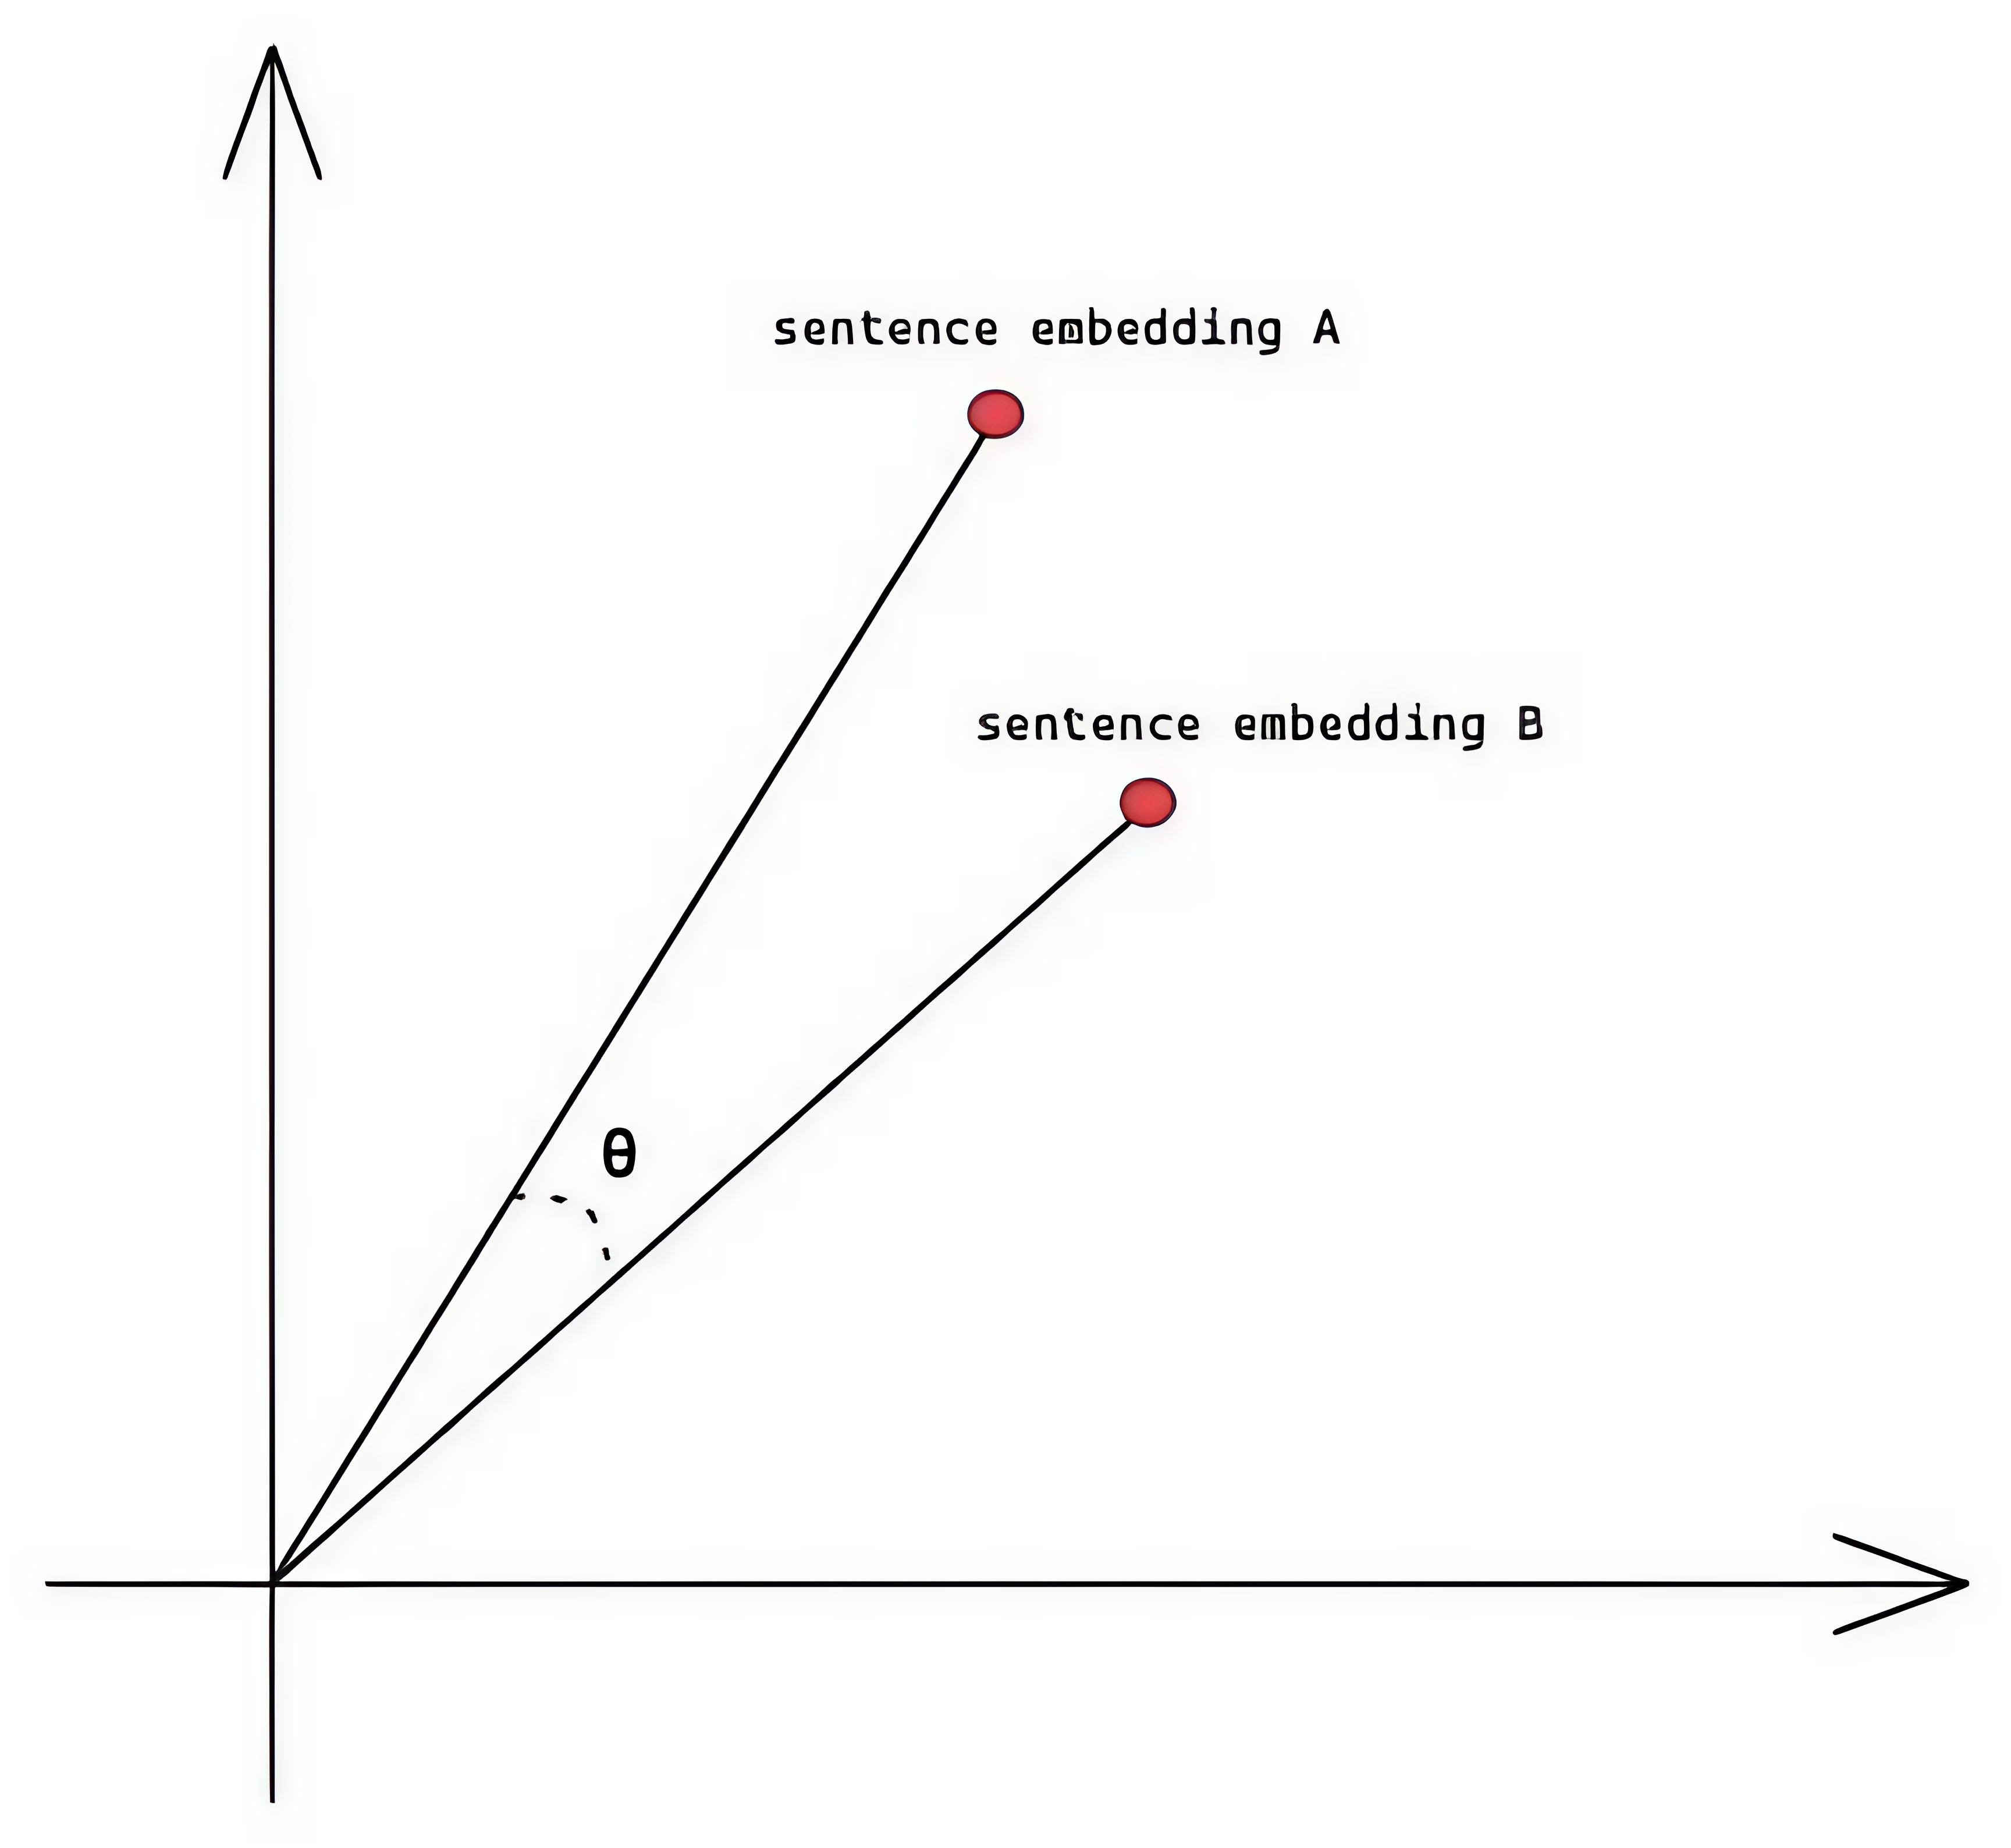
\includegraphics[width=0.6\textwidth]{figures/cosine_similarity.jpeg}
  \caption[Visualization of cosine similarity between two vectors showing how the angle between vectors determines their similarity score]{Visualization of cosine similarity between two vectors showing how the angle between vectors determines their similarity score. \cite{Leys2022}}
  \label{fig:cosine_similarity}
\end{figure}

Such embeddings are crucial for large-scale semantic similarity tasks, such as retrieving documents or knowledge passages relevant to a user query \cite{Reimers2019,Gao2024}. One recent approach is the M3-Embedding model, which was developed to support multilingual and multi-purpose semantic retrieval across varying input granularities. To achieve this, it leverages the encoder architecture of Transformer-based models, as described in Section~\ref{sec:language_models} \cite{Chen2024}.

The training strategy for M3-Embedding follows a pre-training and fine-tuning paradigm. During pre-training, the model was exposed to unlabeled corpora using weak semantic signals such as title-body or title-abstract pairs. To support multilingual capabilities, translation-based datasets were incorporated. Fine-tuning was performed using labeled data from multiple languages, as well as synthetic question-answer pairs generated by \ac{GPT}-3.5 based on multilingual paragraphs \cite{Chen2024}. The model was optimized to determine whether a given query semantically matches a target passage.

To evaluate the performance of sentence embedding models across a wide range of downstream tasks, \citet{Muennighoff2023} introduced the Massive Text Embedding Benchmark (MTEB) \footnote{available under \url{https://huggingface.co/spaces/mteb/leaderboard}}. MTEB consists of 58 datasets covering diverse task categories such as classification, clustering, semantic textual similarity, reranking, retrieval, and summarization. It enables standardized comparisons between embedding models across languages, domains, and input types. Models such as M3-Embedding have achieved strong results on the MTEB benchmark, particularly in multilingual retrieval and reranking tasks. This underlines MTEB’s role as a comprehensive and practical framework for assessing the effectiveness of sentence embeddings across a wide range of real-world applications \cite{Muennighoff2023}.

In summary, sentence embeddings enable the representation of sentences in a vector space while preserving their semantic content. By applying vector operations such as cosine similarity, semantically related texts can be identified efficiently. To achieve high performance on such tasks, recent embedding models like M3-Embedding combine Transformer-based architectures with large-scale pre-training and multilingual fine-tuning.


\section{Retrieval-Augmented Generation}
\label{sec:retrieval_augmented_generation}

As \acp{LM} are trained on static snapshots of large-scale corpora, they are inherently limited in their ability to access up-to-date or domain-specific information that lies outside their training data. Retrieval-Augmented Generation (\ac{RAG}) addresses this limitation by integrating external knowledge sources at inference time. In its simplest form, a \ac{RAG} system consists of three main components: indexing, retrieval, and generation \cite{Gao2024}.

In the indexing step, unstructured text documents are encoded into dense vector representations using embedding models such as M3-Embedding (see Section~\ref{sec:sentence_embeddings}) \cite{Gao2024}. These vectors are then stored in a vector database that supports efficient similarity search using vector algebra \cite{Gao2024,Pan2024}.

\begin{figure}[t]
  \centering
  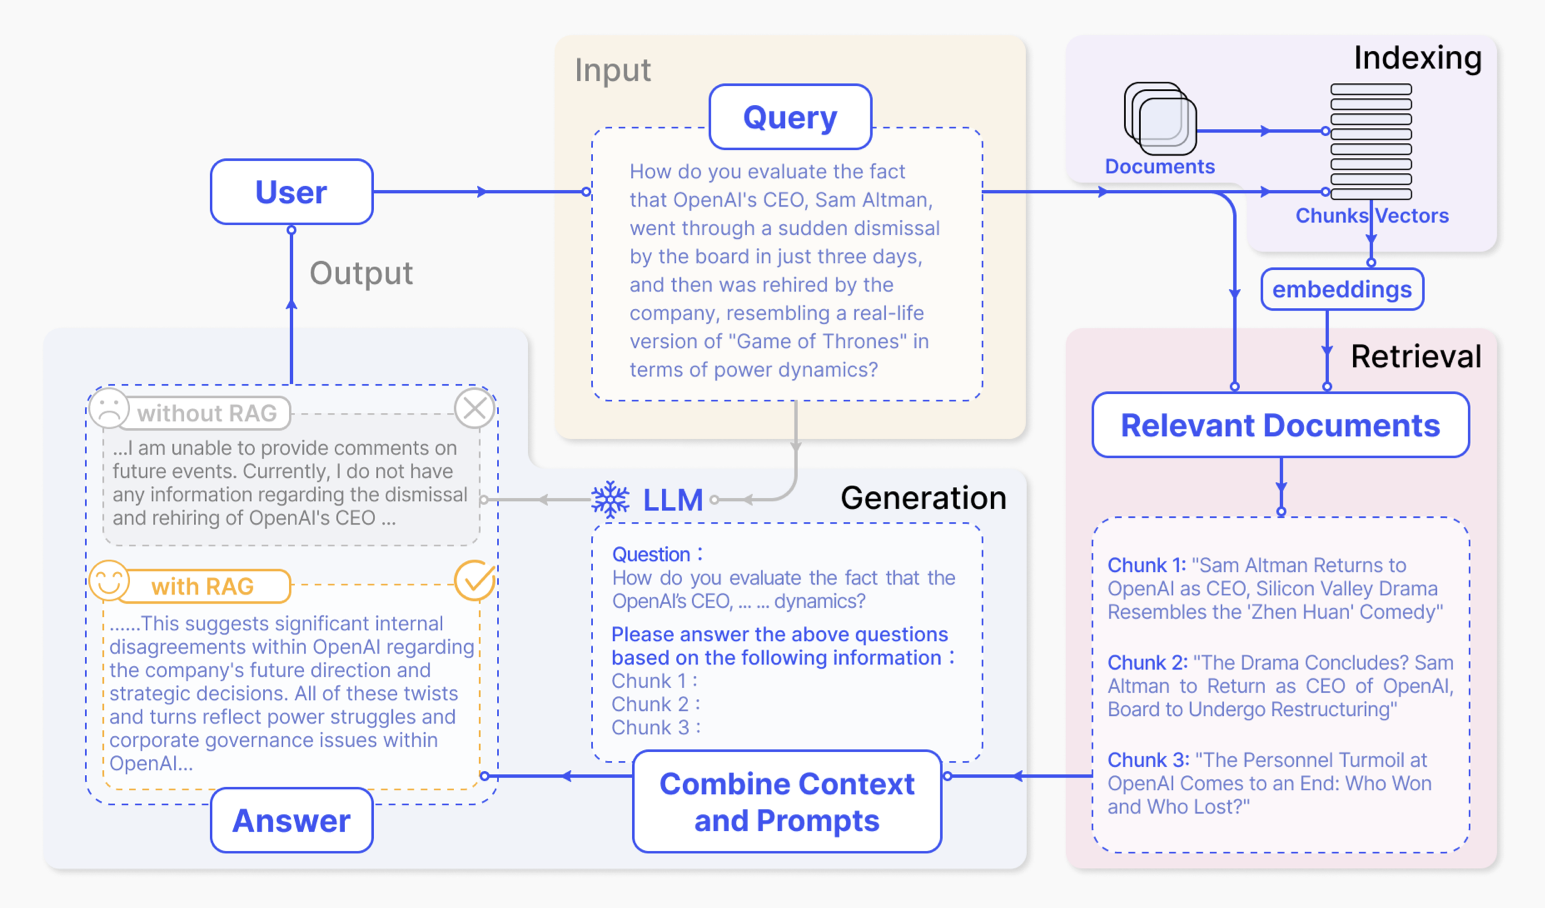
\includegraphics[width=0.8\textwidth]{figures/RAG.png}
  \caption[Overview of the Retrieval-Augmented Generation (RAG) architecture showing the indexing, retrieval, and generation pipeline]{Overview of the Retrieval-Augmented Generation (RAG) architecture showing the indexing, retrieval, and generation pipeline. \cite{Gao2024}}
  \label{fig:rag}
\end{figure}

Figure~\ref{fig:rag} illustrates the architecture of a typical RAG pipeline. While indexing is performed offline, the retrieval and generation steps occur at runtime. During retrieval, the user query is embedded into the same vector space using the same embedding model. Based on this embedding, a similarity search is performed on the vector database, retrieving the most relevant documents. These documents are then inserted into a prompt template along with the original user prompt and, optionally, a system instruction. The resulting prompt is passed to the \ac{LM}, which generates a response informed by the retrieved context \cite{Gao2024}.

A key component of the \ac{RAG} pipeline is the vector database management system (\ac{VDBMS}). Similar to traditional database systems, a \ac{VDBMS} comprises a query processor and a storage manager. The query processor handles vector-based similarity search and optimizes query execution. One widely used example is Qdrant, which employs filtering strategies and adaptive execution paths depending on the size of the vector collection. For large collections, Qdrant avoids brute-force search by applying pre-filtering mechanisms to narrow down the search space. The storage manager handles data persistence and access \cite{Pan2024,Qdrant2025}.

Qdrant organizes data into collections—logical groupings of vectors, often representing a specific domain or project. Each vector can be associated with metadata, called payloads, which support structured filtering during retrieval. The system provides integration with frameworks like Langchain, which facilitates the development of LLM-powered applications \cite{LangChain2025d}. Due to its optimization strategies, Qdrant enables efficient retrieval at scale even for large and complex datasets \cite{Pan2024,Qdrant2025}.

Despite its advantages, RAG systems are not without limitations. \citet{Barnett2024} identify several typical failure points in the RAG pipeline. These include cases where relevant information is missing from the indexed content (FP1), retrieved documents fail to rank highly enough to be included in the context (FP2), or documents are retrieved but discarded during context consolidation (FP3). Even when the relevant information is present, the language model may fail to extract it (FP4) or ignore formatting constraints specified by the user (FP5). Such issues highlight the importance of careful system design, particularly regarding retrieval accuracy, context management, and prompt construction.

In summary, \ac{RAG} provides a scalable and updatable mechanism for incorporating external knowledge into language model outputs. By combining dense semantic embeddings with similarity search in a \ac{VDBMS}, it enables the generation of context-aware responses grounded in up-to-date and domain-specific information.

\section{AI Agents}
\label{sec:ai_agents}

\ac{AI} agents are a more specific form of agents. \citet{Dorri2018} defines an agent as \enquote{(a)n entity which is placed in an environment and senses different parameters that are used to make a decision based on the goal of the entity. The entity performs the necessary action on the environment based on this decision} \cite[S. 28574]{Dorri2018}. The environment describes the setting in which the agent operates and is shaped by factors such as data availability and quality, predictability of outcomes, the degree of change over time, and the continuity of the system state. Parameters refer to the data perceived by the agent, and actions are the set of operations the agent can perform in response.

Agents typically operate based on a decision engine. In the case of \ac{AI} agents, this decision engine is commonly implemented using \ac{LLM} \cite{Sapkota2025,Park2023}. These agents are characterized by a high degree of independence, are tailored to specific tasks, and are capable of adapting their behavior to the current context \cite{Sapkota2025,OpenAI2025}. This distinguishes them from traditional workflow automation, where the sequence of steps is rigidly predefined \cite{Anthropic2024}. \acp{LLM} enable agents for human like behavior due to their internal representation of linguistic and behavioral patterns derived from large scale training corpora \cite{Park2023}.

An \ac{AI} agent system typically consists of an orchestration layer, a language model for decision making and reasoning, and a set of external tools \cite{Wiesinger2025,OpenAI2025}. These components are coordinated by a runtime environment. The orchestration layer is responsible for managing the agent's memory, preparing prompt templates, and handling message flow. This defines which information is passed to the agent and how resulting actions are executed \cite{Wiesinger2025}.

According to \citet{OpenAI2025}, tools can be grouped into three categories: data tools, action tools, and orchestration tools. Data tools are designed to retrieve information from external systems, for example through database queries or web searches. Action tools allow agents to perform operations in external systems such as modifying records in a \ac{CRM}. Orchestration tools include other agents, enabling recursive structures which are further discussed in Section~\ref{sec:multi_agent_systems}. Tools enable agents to interact directly with their environment, thereby enhancing their autonomy and utility.

Each \ac{AI} agent is typically responsible for a clearly defined task and is equipped with a matching tool set. In such scenarios, \citet{Anthropic2024} suggest that an agent should be capable of processing complex inputs, using tools reliably, recovering from errors, and performing task level reasoning and planning. While this setup allows for independence within a task boundary, it limits flexibility beyond that scope unless multi agent orchestration is used \cite{Sapkota2025}.

One example of a reasoning enabled agent framework is ReAct, proposed by \citet{Yao2023}. ReAct combines stepwise reasoning and tool use by prompting the language model to alternate between generating thoughts and performing actions. This process allows agents to maintain a structured internal state composed of thoughts, actions, and observations. Based on this state, the model can iteratively reason about the next step and either call a tool, continue thinking, or terminate execution. The approach is motivated by the observation that human reasoning often interleaves mental reflection with real world interaction \cite{Yao2023}.

To build agents in practice, frameworks such as LangGraph are available. LangGraph is an open source framework for defining agent logic, memory, state tracking, and tool integration using either Python or JavaScript \cite{LangChain2025}. It supports high customizability and is part of the broader LangChain ecosystem \cite{LangChain2025a}.

While \ac{AI} agents provide a high degree of autonomy and adaptability, they are not without limitations. One key challenge lies in their limited ability to model causal relationships, as \acp{LLM} are primarily trained for next-token prediction rather than understanding cause and effect. Additionally, their performance is often highly dependent on the exact wording of the prompt, making outcomes less predictable \cite{Sapkota2025}. \citet{Sapkota2025} also point out that current agents frequently struggle with long-term planning and lack effective mechanisms for recovering from errors. These issues can lead to repetitive behavior or failure to complete complex tasks reliably.

In summary, \ac{AI} agents are autonomous systems that make decisions using language models and interact with their environment through structured tools. They rely on orchestration mechanisms to manage memory and state. Frameworks such as ReAct illustrate one way to guide language model behavior in a controlled reasoning and action loop, but many architectures and implementations exist to serve different use cases.

\section{Multi-Agent-Systems}
\label{sec:multi_agent_systems}

As stated in the previous section, agents are often limited to a single task, making them inflexible when addressing broader problems. A solution to this limitation can be found in \ac{MAS}. The idea is to develop a cost efficient, flexible and reliable system by using multiple agents instead of a single one. In this setup, a complex task is decomposed into multiple simpler tasks. The underlying theory is that solving simpler subtasks leads to more efficient solutions, which in turn compensates for the overhead associated with managing a \ac{MAS} \cite{Dorri2018}.

To make a general \ac{MAS} work, different agents are defined for specific subtasks. In some cases, several agents may handle the same task to increase redundancy or scalability. This requires a well-defined routing strategy within the \ac{MAS}, which can follow either a static or dynamic topology. In a static topology, a leader agent coordinates the other agents and serves as the central point of communication. In contrast, a leaderless \ac{MAS} allows each agent to decide autonomously which agent to invoke next \cite{Dorri2018}.

Leaderless systems introduce greater flexibility, but they also increase the complexity of coordination. Ensuring that all agents contribute effectively toward a shared goal becomes more challenging. Moreover, organizing inter-agent communication and assigning the correct tasks with appropriate inputs becomes increasingly difficult. Fault propagation and fault detection are also harder to manage when multiple agents contribute to a single outcome \cite{Dorri2018}.

These concepts can be extended to \ac{LLM}-based \acp{MAS}. Although single \ac{AI} agents powered by \acp{LLM} can already solve complex tasks, increasing complexity often leads to failure modes such as looping or tool misuse, as noted in Section~\ref{sec:ai_agents} \cite{OpenAI2025}. Therefore, decomposing goals into smaller subtasks managed by specialized agents remains essential \cite{Sapkota2025}.

Each \ac{LLM}-based agent generally shares the same architectural components discussed in Section~\ref{sec:ai_agents}, but in a \ac{MAS}, these components are extended. In particular, the agent state is transformed into a shared state accessible across agents \cite{Sapkota2025}. Each agent must also define a handoff mechanism, which determines the next tool or agent to invoke and the corresponding input or state update. In frameworks like LangGraph, handoffs specify the destination and include a payload that updates the shared state. This shared state is typically implemented as a Python dictionary with predefined fields. Consequently, the orchestration layer becomes more complex, and this complexity is managed by agent frameworks like LangGraph \cite{LangChain2025b}.

\begin{figure}[t]
  \centering
  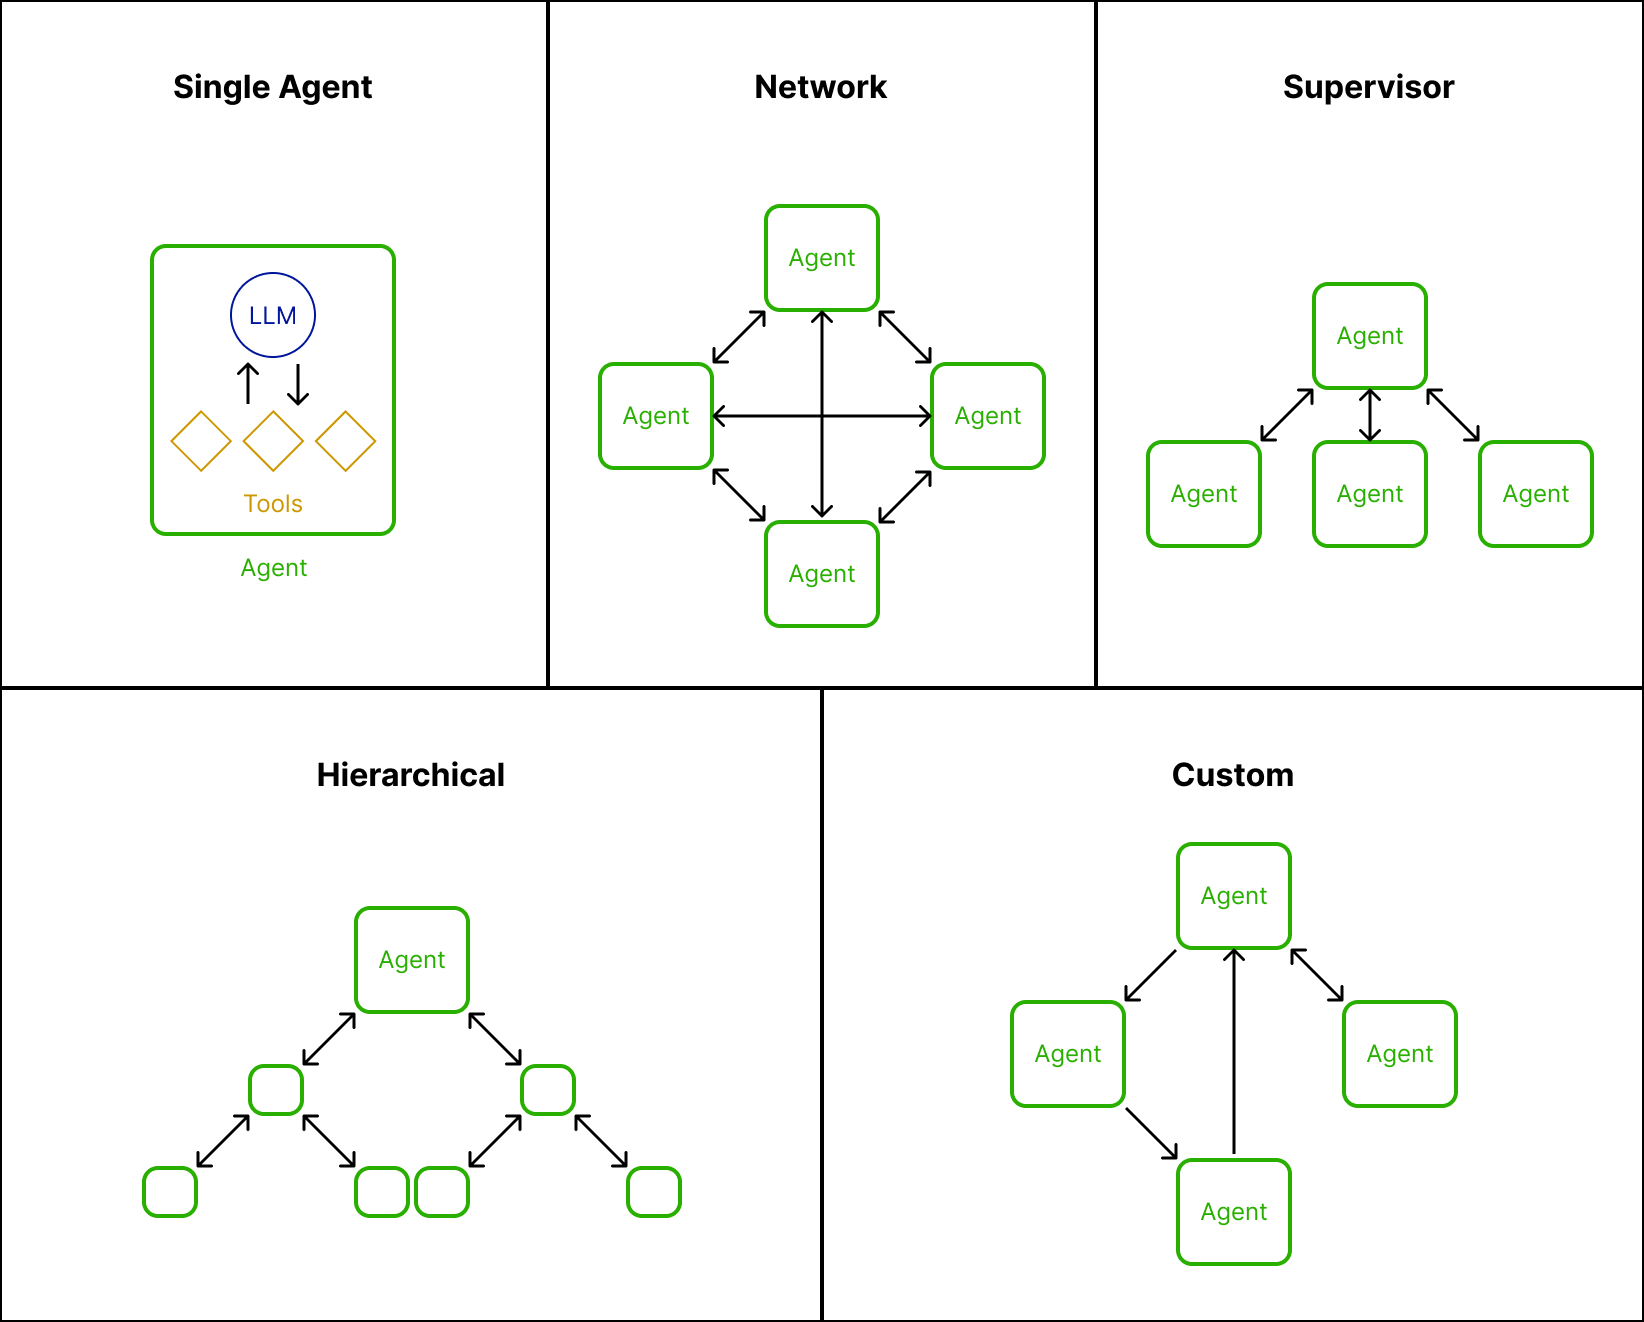
\includegraphics[width=0.8\textwidth]{figures/Multi-agent architectures.png}
  \caption[Example multi-agent architecture patterns showing supervisor, hierarchical, network, and custom patterns for LLM-based multi-agent systems]{Example multi-agent architecture patterns showing supervisor, hierarchical, network, and custom patterns for LLM-based multi-agent systems (self-created after \cite{LangChain2025b})}
  \label{fig:mas_architecture}
\end{figure}

\citet{LangChain2025b} describe several agentic architecture patterns for \ac{LLM}-based \acp{MAS}, which follow classic multi-agent system designs (see Figure~\ref{fig:mas_architecture}). The supervisor pattern represents a leader-follow structure in which a central supervisor agent coordinates the communication with specialized expert agents. These expert agents do not communicate with each other, but only with the supervisor. The hierarchical pattern extends this idea by allowing expert agents to act as intermediate supervisors themselves, enabling a multi-level structure with distributed decision-making responsibilities \cite{LangChain2025b}.

\ac{LLM}-based \acp{MAS} can also follow decentralized, leaderless designs \cite{OpenAI2025,LangChain2025b}. \citet{LangChain2025b} extend this idea through network and custom patterns. In the network pattern, each agent decides independently which other agent to pass control to, effectively managing the process flow itself \cite{LangChain2025b,OpenAI2025}. The custom pattern enables bespoke configurations, such as limiting communication between specific agents or implementing fixed workflows. This flexibility increases modularity and allows for highly specialized agent roles, particularly when implemented with frameworks like LangGraph \cite{LangChain2025b}.

Despite their advantages, \ac{LLM}-based \acp{MAS} also introduce new challenges. First, the lack of causal reasoning in \acp{LLM} becomes more problematic as agents must interact multiple times. Each \ac{AI} agent already introduces uncertainty due to prompt sensitivity and a tendency to enter infinite loops. Using multiple agents compounds this uncertainty and increases the overall system fragility \cite{Sapkota2025}. Furthermore, coordinating communication between agents exposes additional bottlenecks, particularly given the limited context windows of \acp{LLM}, both model-wise and infrastructure-wise \cite{Kwon2023}. Maintaining a shared context and ensuring alignment across agents becomes increasingly difficult \cite{Sapkota2025,Han2025}.

Another critical issue is non-composability. Because \acp{LLM} may respond unpredictably, introducing a new agent into the system does not guarantee that it will be utilized effectively. Instead, it may increase prompt complexity without improving performance. As the number of agents grows, tracing the source of errors also becomes harder due to the sensitivity of \acp{LLM} to prompt changes. In addition, the field of \ac{LLM}-based \acp{MAS} remains relatively immature, which contributes to the lack of standardized solutions \cite{Sapkota2025}.

Nonetheless, recent work has begun to address some of these problems. For instance, integrating retrieval-augmented generation can help mitigate reasoning gaps by supplying agents with relevant external knowledge. The use of deterministic tools within the agent loop also improves reliability. Monitoring and auditing tools can support root cause analysis, and simulation tools may enhance causal awareness. Communication challenges may be addressed through improved memory architectures and coordination mechanisms \cite{Sapkota2025}.

In summary, \ac{LLM}-based \acp{MAS} offer a promising approach to solving complex problems through the collaboration of multiple specialized \ac{AI} agents. These systems can be organized hierarchically, networked, or in fully custom configurations. While they provide flexibility and scalability, they also introduce challenges such as error amplification, coordination overhead and reduced traceability. As research in this area progresses, new techniques and tools continue to emerge to address these limitations and improve the robustness of such systems.

\section{Agent Design}
\label{sec:agent_design}

As the field of \ac{AI} agent research matures, so does the understanding of when and how to use such agents effectively. In general, \citet{OpenAI2025} recommend employing \ac{AI} agents when deterministic rules fall short, particularly when the problem cannot be easily formalized into a ruleset. This is especially true in cases involving complex decision-making or unstructured data, where \ac{AI} agents are likely to outperform rule-based systems \cite{OpenAI2025}.

As described in Section~\ref{sec:ai_agents}, \ac{AI} agents are typically designed for a single task and constrained by the context they can process. These limitations become apparent when agents begin to fail at following instructions or when their decision-making performance degrades. Some problems are inherently too complex in terms of context or tool usage, leading to tool overload. In such cases, task and tool responsibilities can be decomposed across a \ac{MAS}. This approach is particularly useful when problems require complex logic that benefits from being broken into subtasks \cite{OpenAI2025,LangChain2025b}. However, \ac{LLM}-based \acp{MAS} should be used thoughtfully, as their architecture entails high cost and complexity \cite{Hadfield2025}.

Regarding agent design, \citet{Anthropic2024} emphasize prioritizing simplicity over complexity. They argue that agentic systems should strike a balance between latency and task performance. Similarly, \citet{Hadfield2025} propose treating agent systems like human teams. Tasks should be concise, actions clearly defined, and the context understandable to humans, given that \acp{LLM} are trained on human-generated text. Context compression is another recommended technique to keep prompts manageable and more interpretable \cite{Hadfield2025}. These principles support the hypothesis proposed by \citet{Anthropic2024}, which suggests that if a human can solve a task, an \ac{AI} agent should be able to solve it as well, provided the problem is stated clearly. In this spirit, \citet{OpenAI2025} advise capturing edge cases early to improve agent robustness and keeping components modular and composable, particularly in \ac{LLM}-based \acp{MAS}.

Since \acp{LLM} remain prompt-sensitive, effective prompt engineering is essential. \citet{Anthropic2024} suggest considering the training background of the model. As \acp{LM} are primarily trained on prose and optimized to generate coherent text, prompts should closely resemble the structure and format of natural language. Unnecessary formatting should be avoided, as it may reduce performance. Furthermore, \citet{Hadfield2025} recommend teaching agents how to orchestrate the \ac{MAS}, including a guided reasoning process. Overall, prompt clarity and structure are key to agent effectiveness \cite{OpenAI2025}.

As outlined in Section~\ref{sec:language_models}, one effective prompting strategy is in-context learning. When applying one-shot or few-shot prompting, decisions must be made regarding the number, order, format, and similarity of the examples \cite{Schulhoff2025}. Various prompting styles such as role prompting, style prompting, or emotion prompting can also influence outcomes. Another popular method is \ac{CoT} prompting, which encourages the model to reason step by step. Few-shot \ac{CoT} extends this by incorporating worked-out examples. Automatic prompt optimization can further improve agent performance \cite{Schulhoff2025}.

\citet{Schulhoff2025} evaluate various prompting strategies using the MMLU benchmark, which is closely related to the MMLU-Pro benchmark discussed in Section~\ref{sec:language_models}. Their findings show that few-shot \ac{CoT} prompting performed best, while zero-shot \ac{CoT} performed worst. These results align with earlier findings by \citet{Brown2020}, who described \acp{LM} as effective few-shot learners.

In addition to prompt engineering, well-designed tools are crucial for tasks requiring interaction with external systems or knowledge \cite{OpenAI2025}. According to \citet{Anthropic2024}, tool descriptions must be as carefully engineered as the prompts themselves. \acp{LLM} must be able to generate structured handoffs from unstructured input based on the tool descriptions. Tools should be tested thoroughly, and their usage logged for traceability. Making tools foolproof can reduce the likelihood of errors and support more robust performance \cite{Anthropic2024}.

Once agents are deployed, performance iteration is key. \citet{Hadfield2025} recommend beginning evaluation with small examples and incorporating human oversight to identify errors not easily caught through automation. In particular, tool execution should be traced and debugged to identify weak points. One example of a platform for this kind of engineering is Langfuse \cite{LGFT2025}.

In summary, given the limitations of \acp{LLM}, careful agent design is essential. Effective \ac{AI} agents and \ac{LLM}-based \acp{MAS} must be modeled after human problem-solving processes and supported through robust prompt and tool engineering. When well designed, such systems can effectively address complex tasks \cite{Hadfield2025}.

\chapter{Related Work}
\label{ch:related_work_chapter}

This chapter presents the current state-of-the-art training and benchmarking datasets as well as various approaches in the field of information extraction, with a particular focus on solutions in the area of \ac{cIE}. Section~\ref{sec:related_datasets} discusses the \textit{REBEL dataset}, one of the first large-scale datasets for open and closed information extraction, followed by the \textit{synthIE dataset}, a synthetically generated resource based on models from the \textit{GPT-3.5} family. Section~\ref{sec:related_approaches} outlines different methodological approaches, ranging from transformer fine-tuning and prompt tuning to the use of \ac{AI} agents for open and closed information extraction.

\section{Related Datasets}
\label{sec:related_datasets}

Datasets are crucial for training, and especially for evaluating, approaches in the domain of \ac{cIE}. This requires not only high-quality but also large-scale datasets \cite{Josifoski2023}. The \textit{REBEL dataset} was created by analyzing Wikipedia abstracts and extracting all hyperlinks. Additionally, a RoBERTa-based \ac{LM} was used to filter whether a text entails the extracted triples by leveraging RoBERTa’s entailment prediction capabilities. This results in a large-scale, automatically created dataset in which noise is accepted. Accordingly, the \textit{REBEL dataset} can be classified as a silver-standard dataset. A silver-standard dataset refers to a dataset that is automatically generated without human validation. As a result, such datasets typically contain a higher level of noise and lower reliability compared to human-annotated (gold-standard) datasets \cite{HuguetCabot2021}.

To address issues with noise and predicate frequency skewness in the \textit{REBEL dataset}, \citet{Josifoski2023} introduced the \textit{synthIE dataset}. The idea is to leverage the text generation capabilities of \acp{LLM} from the \textit{GPT-3.5} series to generate texts that correlate with expected triples \cite{Josifoski2023}. \citet{Josifoski2023} created an unskewed set of triples based on a subset of Wikidata and prompted these with corresponding instructions into \texttt{text-davinci-003} (based on InstructGPT) or \texttt{code-davinci-002} (a base GPT model) \cite{Josifoski2023,OpenAI2025a}. Human-annotated samples revealed that, in contrast to the \textit{REBEL dataset}, most of the triples within the generated texts of the \textit{synthIE dataset} were detectable \cite{Josifoski2023}.

Both the \textit{REBEL dataset} and the \textit{synthIE dataset} provide pairs of natural language text and corresponding knowledge triples. These triples include not only the surface forms of entities and predicates as they appear in the text, but also an identifier for the corresponding entry in Wikidata. This enables evaluation for \ac{cIE} approaches on both datasets.

In summary, \citet{HuguetCabot2021} and \citet{Josifoski2023} provided large-scale datasets. The \textit{synthIE dataset} is of higher quality and thus yields better results when used for evaluation. Both the \textit{REBEL dataset} and the \textit{synthIE dataset} offer extensive training, validation, and test splits, serving as a foundation for the development of approaches in \ac{cIE}.

\section{Related Approaches}
\label{sec:related_approaches}

As outlined in Section~\ref{sec:closed_information_extraction}, open and closed information extraction methods follow either pipeline or joint approaches. These rely on a broad variety of techniques, ranging from table-filling with tag probability learning to LSTM-based models and encoder-decoder architectures \cite{Zhang2022,Angeli2015,Trisedya2019}. With the rise of transformer-based Seq2Seq models, recent approaches predominantly implement transformer architectures \cite{Josifoski2021,Josifoski2023,Moeller2024}.

Even before the emergence of \acp{LLM}, transformer models demonstrated superior performance compared to other state-of-the-art methods. A prominent example is the \textit{REBEL model} trained on the \textit{REBEL dataset} \cite{HuguetCabot2021}. By fine-tuning a BERT model with texts as input and triples as output, \citet{HuguetCabot2021} achieved superior results on benchmarking datasets, presenting a flexible relation extraction model.

\citet{Josifoski2021} introduced \textit{GenIE}, adapting the REBEL framework for \ac{cIE}. In their approach, \citet{Josifoski2021} constrained the decoding process in the BART-based \ac{LM} so that it would generate only outputs aligned with entities and relations from the underlying knowledge base Wikidata. They applied output linearization by introducing special tokens to delimit subject, predicate, and object. Furthermore, a constrained beam search was implemented to ensure that only valid tokens from Wikidata could be generated. This method outperformed a traditional pipeline consisting of named entity recognition, entity disambiguation, relation classification, and triplet classification \cite{Josifoski2021}.

Building upon \textit{GenIE} and the quality of the \textit{synthIE dataset}, \citet{Josifoski2023} proposed the \textit{synthIE model}. While following GenIE’s architecture, the \textit{synthIE model} replaces BART with Flan-T5 due to broader availability of pre-trained configurations. The best-performing \textit{synthIE model}, trained on the training split of the \textit{synthIE dataset}, surpassed the \textit{GenIE} model trained on the \textit{REBEL dataset} (also based on Flan-T5) by over 0.8 macro-F1 on the \textit{synthIE-text} evaluation set. This result highlights the strong correlation between the quality of training and benchmarking datasets and overall model performance \cite{Josifoski2023}.

Exploring foundation models that can be fine-tuned or prompt-engineered, \citet{Xue2024} proposed a pipeline approach using fine-tuned \acp{LLM} for relation extraction, subject identification, and triplet fact extraction. In contrast, \citet{Chen2024} introduced a prompt-tuning method for joint optimization. The approach by \citet{Xue2024} achieved a 10\% F1-score improvement on the document-level open information extraction dataset Re-DocRED compared to prior models. Moreover, they demonstrated that base models like ChatGPT were clearly outperformed by fine-tuned models \cite{Xue2024}.

\citet{Chen2024}, on the other hand, applied prompt tuning for open information extraction across sentence boundaries rather than full documents. Their results showed that well-designed prompt tuning strategies can match the performance of fine-tuned approaches. \citet{Chen2024} did not compare their model to other approaches presented in this work. It should be noted that both \citet{Chen2024} and \citet{Xue2024} used datasets focused on open information extraction rather than \ac{cIE}. As a result, their performance metrics are not directly comparable to approaches evaluated on the \textit{REBEL dataset} or the \textit{synthIE dataset}. In general, comparing models trained and tested on different datasets provides limited insight into their relative strengths, particularly in task-specific contexts like \ac{cIE}.

The most similar approach to this work is \textit{AgentRE} by \citet{Shi2024}. With advances in AI agents, \citet{Shi2024} proposed a single-agent framework for open information extraction. The agent had access to a retrieval module and a memory module. The retrieval module provided relevant samples and context from a knowledge graph, including sample triples and relation descriptions. The memory module stored correct and incorrect extractions and supported self-reflection with the help of the \ac{LLM}. The agent orchestrated these components and extracted valid triples from input texts \cite{Shi2024}.

\textit{AgentRE} was evaluated on several benchmark datasets unrelated to the \textit{REBEL dataset} or the \textit{synthIE dataset}. The main dataset, \textit{SciERC}, is limited and outdated \cite{Luan2018}. Experiments using \texttt{GPT-3.5 Turbo} and a reasoning-enhanced \texttt{LLaMA-2-7B} model showed that \textit{AgentRE} outperformed other methods on most datasets, highlighting the potential of AI agents for information extraction \cite{Shi2024}. However, as with other approaches, the implications for \ac{cIE} remain limited.

In summary, recent advances in \ac{LLM} research have demonstrated improvements in both open and closed information extraction. A range of approaches—fine-tuning, prompt tuning, and agent-based frameworks—can address the problem. Furthermore, the importance of high-quality datasets for training and especially for benchmarking in \ac{cIE} has been clearly demonstrated. However, many of the approaches discussed either do not use the latest \acp{LLM} or do not directly address \ac{cIE}, thus limiting their applicability to this work.

\chapter{Approach}
\label{ch:approach}

This work introduces a novel approach to \ac{cIE} based on \acp{MAS}. The core idea is to evaluate both the pipeline and the joint approach to \ac{cIE} through multiple specialized agents. To fulfil this task, agents must be capable of accessing and retrieving data directly from the knowledge graph. For this reason, the concept of tools is employed.

Instead of relying on model fine-tuning, the proposed \ac{MAS} is designed entirely around prompt tuning and in-context learning. The overarching goal is to create a system that can be applied in real-world scenarios. In this context, real-world applicability means that the system must be able to handle diverse text types and operate with different knowledge graphs. The decision to focus on in-context learning is based on findings by \citet{Brown2020}, who demonstrated that this method can outperform domain-specific fine-tuned models. Moreover, recent advancements in large language models show that new architectures can either surpass previous models or achieve similar performance with fewer parameters \cite{MetaAI2025,Chiang2024}, which suggests enhanced capabilities for in-context learning. Details on the language models used in this work are provided in Section~\ref{subsec:eval_language_models}.

An iterative development process was followed to design and evaluate a range of \acp{MAS}, drawing on the best practices discussed in Section~\ref{sec:agent_design}. To the best of the author's knowledge, no prior research has proposed a multi-agent system specifically for \ac{cIE}. This made the iterative process essential. It enabled the identification of limitations in early designs and informed subsequent refinements. As a result, four core architectures emerged. The \textit{baseline architecture}, described in Section~\ref{subsec:baseline}, follows a strict pipeline-oriented design. The \ac{SSA} and \ac{SSSA} architectures, outlined in Sections~\ref{subsec:supervisor} and~\ref{subsec:simplified_splitted_supervisor}, introduce task-splitting mechanisms based on the baseline. In contrast, the \textit{ReAct architecture} in Section~\ref{subsec:react} simplifies the system by consolidating all responsibilities into a single agent while retaining tool usage. Finally, the \textit{network architecture}, detailed in Section~\ref{subsec:network}, demonstrates how expert agents can autonomously define and manage the system's flow.

In addition to agent structures, several tools were developed. The most important tool for \ac{cIE} is the \textit{URI retrieval tool} (Section~\ref{subsec:uri_retrieval}), which maps search terms to corresponding URIs. To further increase knowledge graph integration, additional tools were designed: the \textit{network traversal tool} (Section~\ref{subsec:network_traversal}), a \textit{semantic validation component} (Section~\ref{subsec:semantic_validation}), and a \textit{Turtle-to-label converter} (Section~\ref{subsec:turtle_to_label}). However, the presence of a tool does not imply that it was integrated into every architecture.

Agents are implemented as calls to \acp{LLM} using a prompt template, which is dynamically filled with selected input fields. In principle, many \acp{LLM} supported in LangChain offer structured output parsing, where responses can be automatically mapped to predefined schemas \cite{LangChain2025e}. Since this functionality was not consistently supported across all models, this work instead relies on parsing structured data directly from the model-generated text. To enable this, the \ac{LLM} is instructed to output specific XML tags containing information about the next agent, the final output, instructions for subsequent agents, or the input for tools.

It is important to note that all architectures were iteratively refined with regard to prompt design and tool usage, especially those that demonstrated promising results. As previously mentioned, the development of tools was driven by the iterative nature of the system design. Consequently, certain tools were designed exclusively for specific architectures. Details on which tools were used with which architectures are provided in Section~\ref{sec:evaluation_configurations}.

\section{Agent Architectures}
\label{sec:agent_architectures}

This section presents the different agent architectures developed in this work. Each architecture is described with respect to the specific agents involved, the overall system flow, and the internal handoff mechanisms between agents. Furthermore, the definition of agent state and the process of passing control or data from one agent to another are outlined for each architecture. Understanding these architectural variations is essential for evaluating the trade-offs between modularity, control, and performance in multi-agent systems for \ac{cIE}.

\subsection{Baseline Architecture}
\label{subsec:baseline}

\begin{figure}[tp]
  \centering
  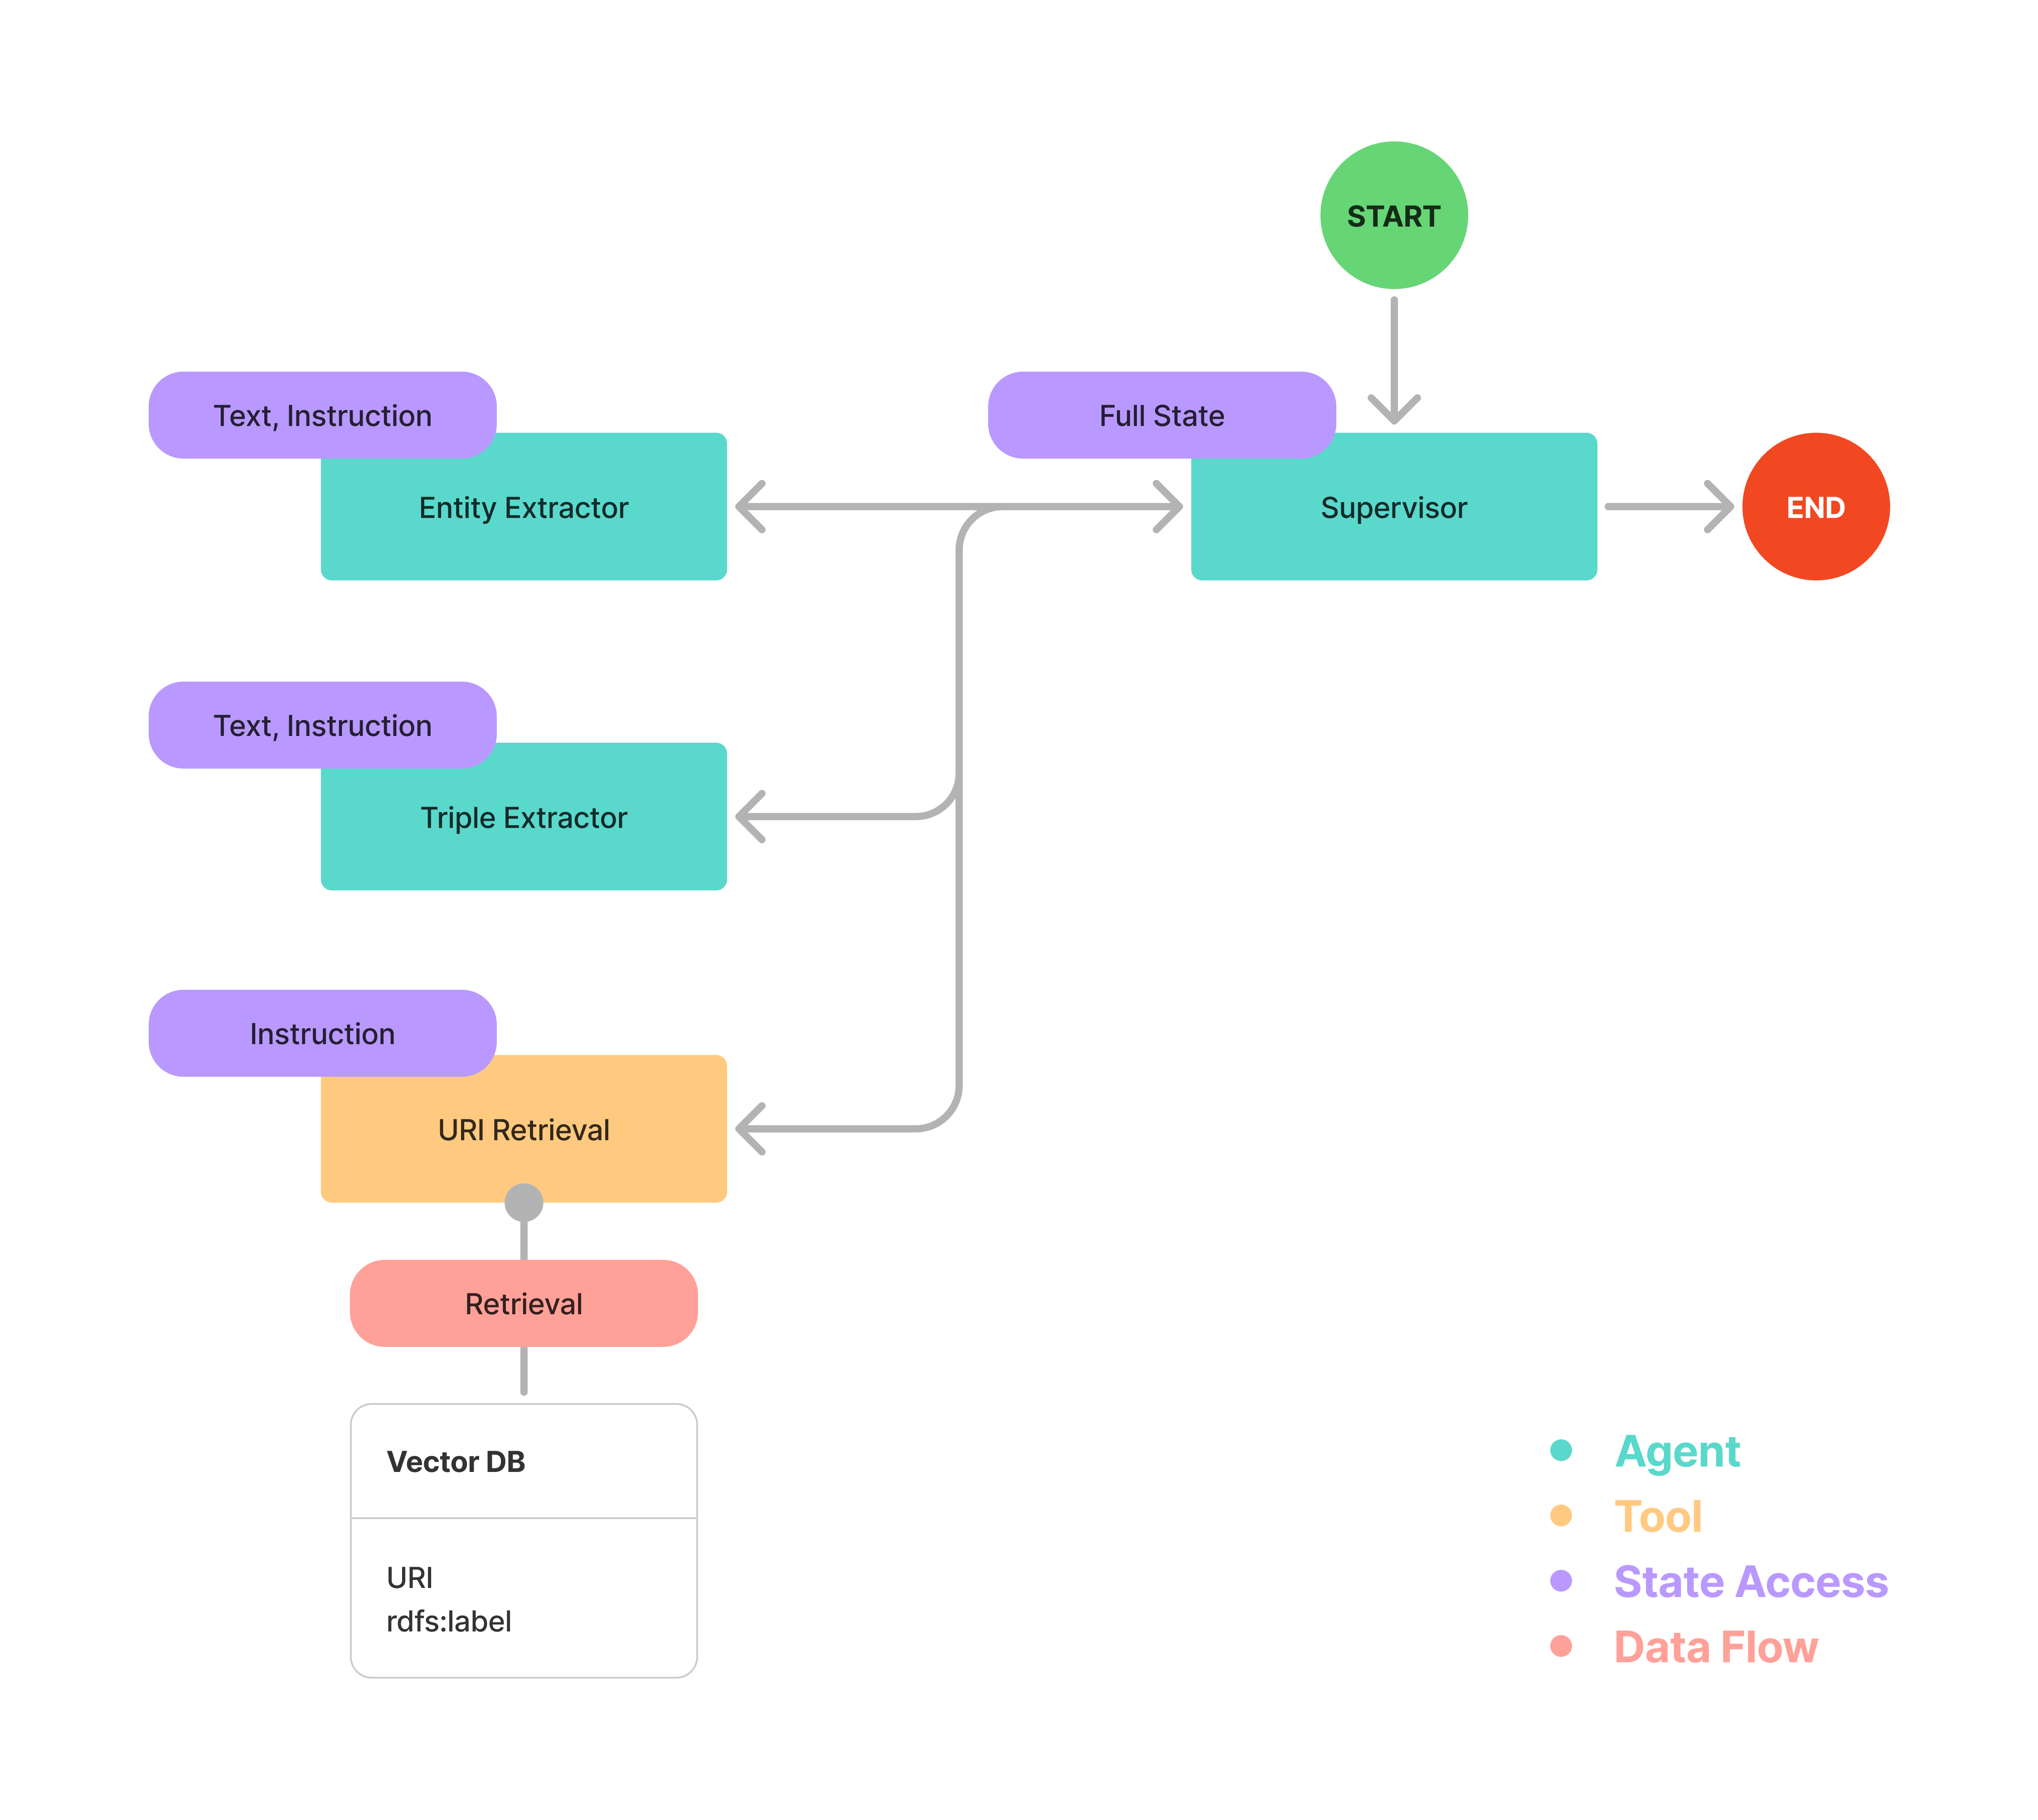
\includegraphics[width=0.7\textwidth]{figures/Baseline Architecture.png}
  \caption[Baseline architecture showing the pipeline approach with specialized agents for each step of the closed information extraction process]{Baseline architecture showing the pipeline approach with specialized agents for each step of the closed information extraction process (self-created)}
  \label{fig:baseline_architecture}
\end{figure}

The \textit{baseline architecture} represents the initial implementation of a \ac{MAS} for closed information extraction in this work. It follows a classical pipeline approach to \ac{cIE} by introducing two specialized agents: one for extracting entities and relations, and another for disambiguating and forming triples. This reflects the multi-agent principle of decomposing complex tasks. Closed information extraction is commonly considered such a task \cite{Josifoski2021}. Additionally, the architecture implements a supervisor agent that aligns with the supervisor pattern and coordinates the workflow and communication between agents. At this stage, the \textit{URI retrieval tool} is already integrated to map the free-text triples to corresponding URIs. An overview of this architecture is shown in Figure~\ref{fig:baseline_architecture}.

At the core of the \textit{baseline architecture} lies the concept of state. The state consists of three main fields: \texttt{text}, \texttt{messages}, and \texttt{instruction}. The \texttt{text} field contains the document or sentence being processed. The \texttt{messages} field stores all exchanged messages. This allows the supervisor agent to access the message history, avoid repetition, and support targeted reasoning. The \texttt{instruction} field is used to provide task-specific input for tools or agents.

Because this is a supervisor-based architecture, orchestration and routing are fully managed by the \textit{supervisor agent}. It is the only agent with access to the complete system state. In addition to coordinating the sequence of operations, the supervisor is responsible for validating intermediate results and formatting the final output. After invoking the specialized agents for entity and triple extraction, the supervisor assesses the quality of the returned results. If needed, it can initiate additional reasoning steps or repeat certain parts of the process. This includes re-running agents to improve disambiguation. The supervisor agent uses the \texttt{instruction} field to send specific prompt inputs to other agents. When a triple is produced by the triple extractor, the supervisor constructs search terms and queries the \textit{URI retrieval tool}. Based on the retrieved URIs, the supervisor composes a valid Turtle output.

To coordinate agents and parse their responses, the \textit{baseline architecture} relies on XML tags that delimit structured output elements such as the next agent or the instruction. This approach addresses the challenge that not all models and frameworks used in CIExMAS support structured outputs. As a result, parsing agent responses based on explicitly marked tags is a core strategy that is consistently applied across all architectures and configurations.

The \textit{entity} and \textit{triple extraction agents} are entirely based on prompt engineering. Initially, both agents were prompted with simple instructions requesting entity or triple extraction respectively. Over time, these agents are expected to perform increasingly well on their narrow tasks as prompts are refined iteratively. Details about the overall prompt engineering process are described in Section~\ref{sec:iterative_prompt_engineering}.

Overall, this baseline design results in a pipeline, in case any result is error-free. First, entities are extracted. Then, triples are constructed. The supervisor retrieves matching URIs and generates a final Turtle output. If this process fails, for example due to missing or incorrect entities or predicates, the supervisor can repeat parts of the workflow. This flexibility allows the architecture to extend beyond a purely linear structure and reduces the risk of error propagation.

\subsection{Splitted Supervisor Architecture}
\label{subsec:supervisor}

\begin{figure}[tp]
  \centering
  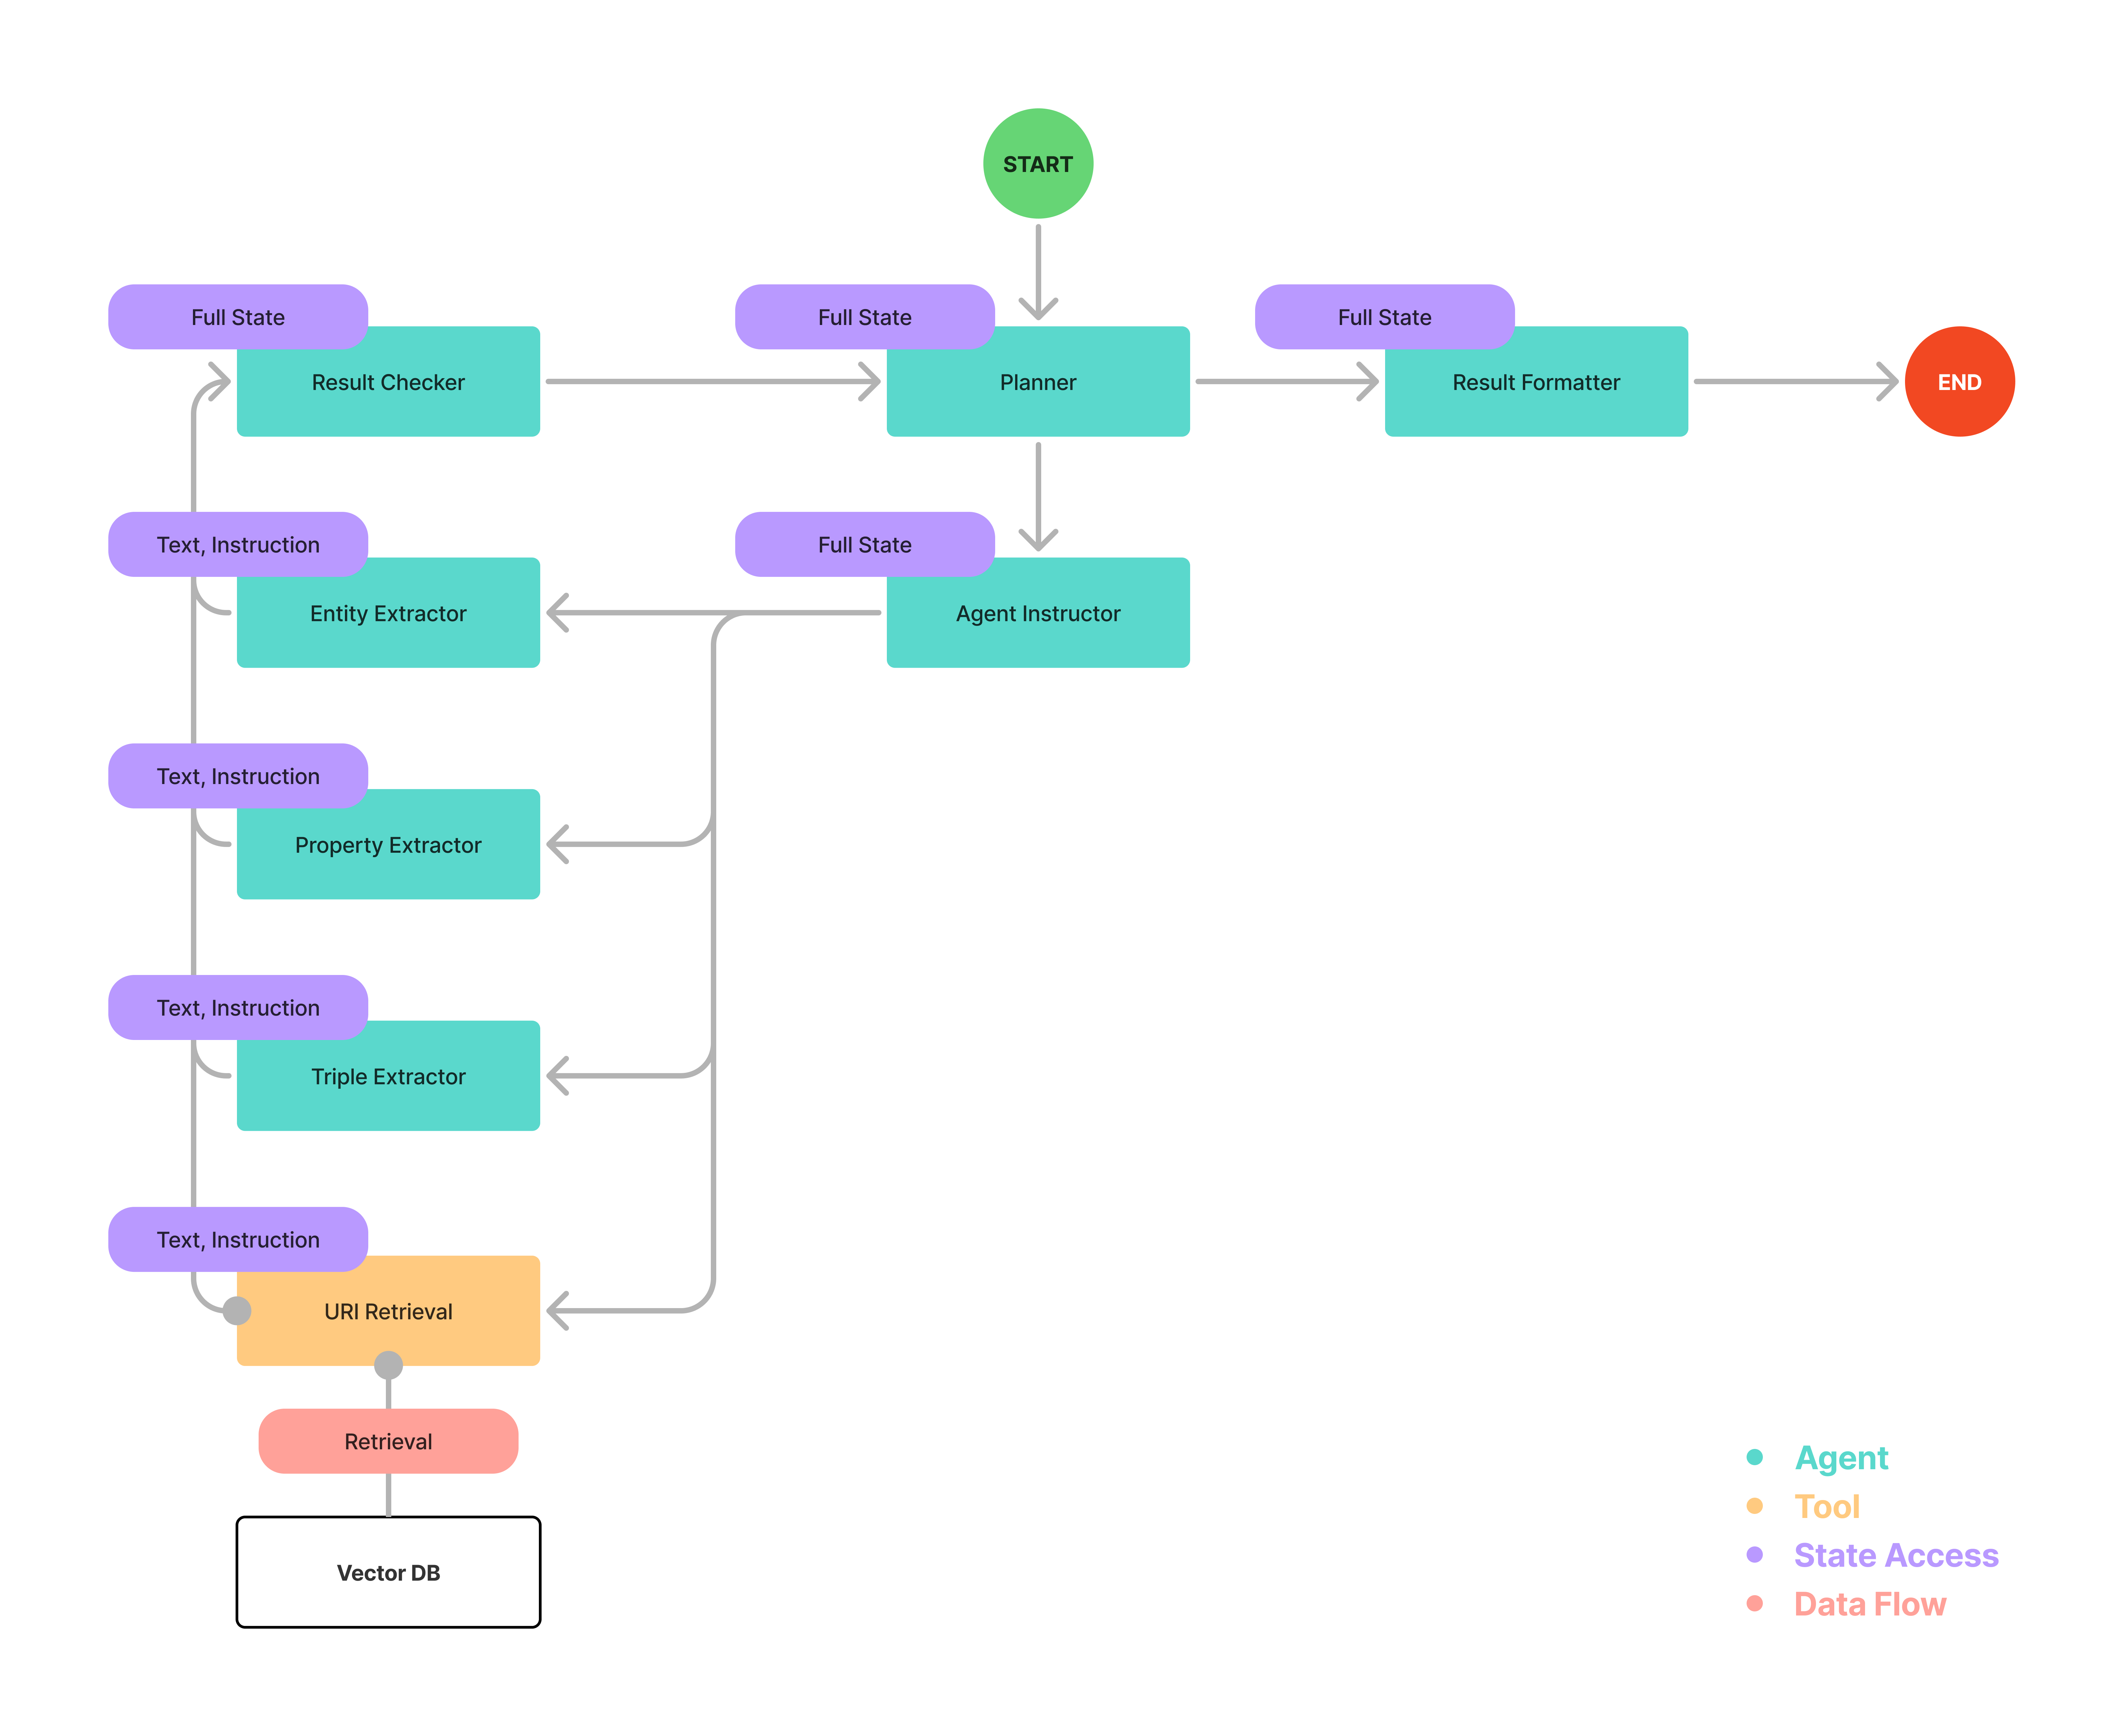
\includegraphics[width=0.7\textwidth]{figures/Splitted Supervisor Architecture.png}
  \caption[Splitted supervisor architecture showing the decomposition of the supervisor agent into specialized sub-agents for better task management]{Splitted supervisor architecture showing the decomposition of the supervisor agent into specialized sub-agents for better task management (self-created)}
  \label{fig:splitted_supervisor_architecture}
\end{figure}

Building on the \textit{Baseline Architecture}, the \textit{Splitted Supervisor Architecture} (\ac{SSA}) extends the supervisor pattern by decomposing the central supervisor agent into a series of smaller, specialized agents. In both setups, the main responsibilities remain the same: planning the task, routing it to the appropriate agent or tool with the correct instruction, evaluating the outputs, and either refining the plan or producing a final \texttt{turtle} string. However, this process proves to be complex, especially if iterative refinement over the \ac{cIE} task is intended. The \ac{SSA} addresses the limitations of \acp{LLM} that struggle with processing many instructions at once or face context window restrictions as prompt sizes grow. As a result, the supervisor role is split into four distinct agents: \textit{planner}, \textit{agent instructor}, \textit{result checker}, and \textit{result formatter}. Additionally, a new \textit{property extractor} agent complements the existing specialized agents for entity and relation extraction. Because the property extractor was added later in the iterative process, further evaluation is discussed in Section~\ref{subsec:error_message_incorporation}. An overview of this architecture is provided in Figure~\ref{fig:splitted_supervisor_architecture}.

To support the expanded supervision logic, the system state is redesigned. In addition to the existing \texttt{text} and \texttt{instruction} fields, the \ac{SSA} state includes \texttt{call\_trace}, \texttt{results}, and \texttt{comments}. The \texttt{call\_trace} field stores a log of which agent or tool was invoked with which input and helps the \textit{agent instructor} track system flow. The \texttt{results} field collects outputs from both the specialized agents and the \textit{URI Retrieval Tool}. Meanwhile, \texttt{comments} serves as a space for internal notes from supervision agents. This structure enables a clean separation between the core \ac{cIE} results and the surrounding orchestration logic. Agents can also benefit from this pre-structured representation, which facilitates reasoning over prior steps.

At the heart of the \ac{SSA} is the \textit{planner agent}. It initiates the overall process, develops a step-by-step plan, and decides at each stage whether to proceed or terminate by delegating final output creation to the \textit{result formatter}. If the next action requires agent involvement, the \textit{agent instructor} translates the planner's intention into a concrete agent call with a matching instruction. This modularity allows each agent to specialize: planning agents can focus on sequencing, while instructors handle syntactic formatting. The \textit{result formatter} follows the same philosophy and is responsible for generating the final output in valid \texttt{turtle} syntax. In doing so, it combines all partial outputs such as triples and \acp{URI}.

Functioning as the quality control unit, the \textit{result checker agent} plays a critical role in this architecture. It evaluates whether the specialized agents are producing meaningful results and identifies missing or incorrect elements. In doing so, it provides feedback to the \textit{planner agent} and encourages iterative improvement over the extraction process.

The specialized agents for entity and relation extraction behave similarly to those in the baseline setup, with adjustments made regarding where their results are stored in the updated state. The new \textit{property extractor} agent was introduced in line with design practices discussed in Section~\ref{sec:agent_design}. Its task is to extract properties from the text, which were previously identified as part of relation extraction. The \textit{URI Retrieval Tool} remains conceptually the same as in the \textit{Baseline Architecture}, though its outputs are now written to the centralized \texttt{results} field.

In summary, the \ac{SSA} is a more modular interpretation of the supervisor pattern, aimed at breaking down complex orchestration into simpler, manageable components. The state has been enhanced to support this expansion by providing more transparency and structure, enabling a greater degree of control and adaptability across the agent system.

\subsection{Simplified Splitted Supervisor Architecture}
\label{subsec:simplified_splitted_supervisor}

\begin{figure}[tp]
  \centering
  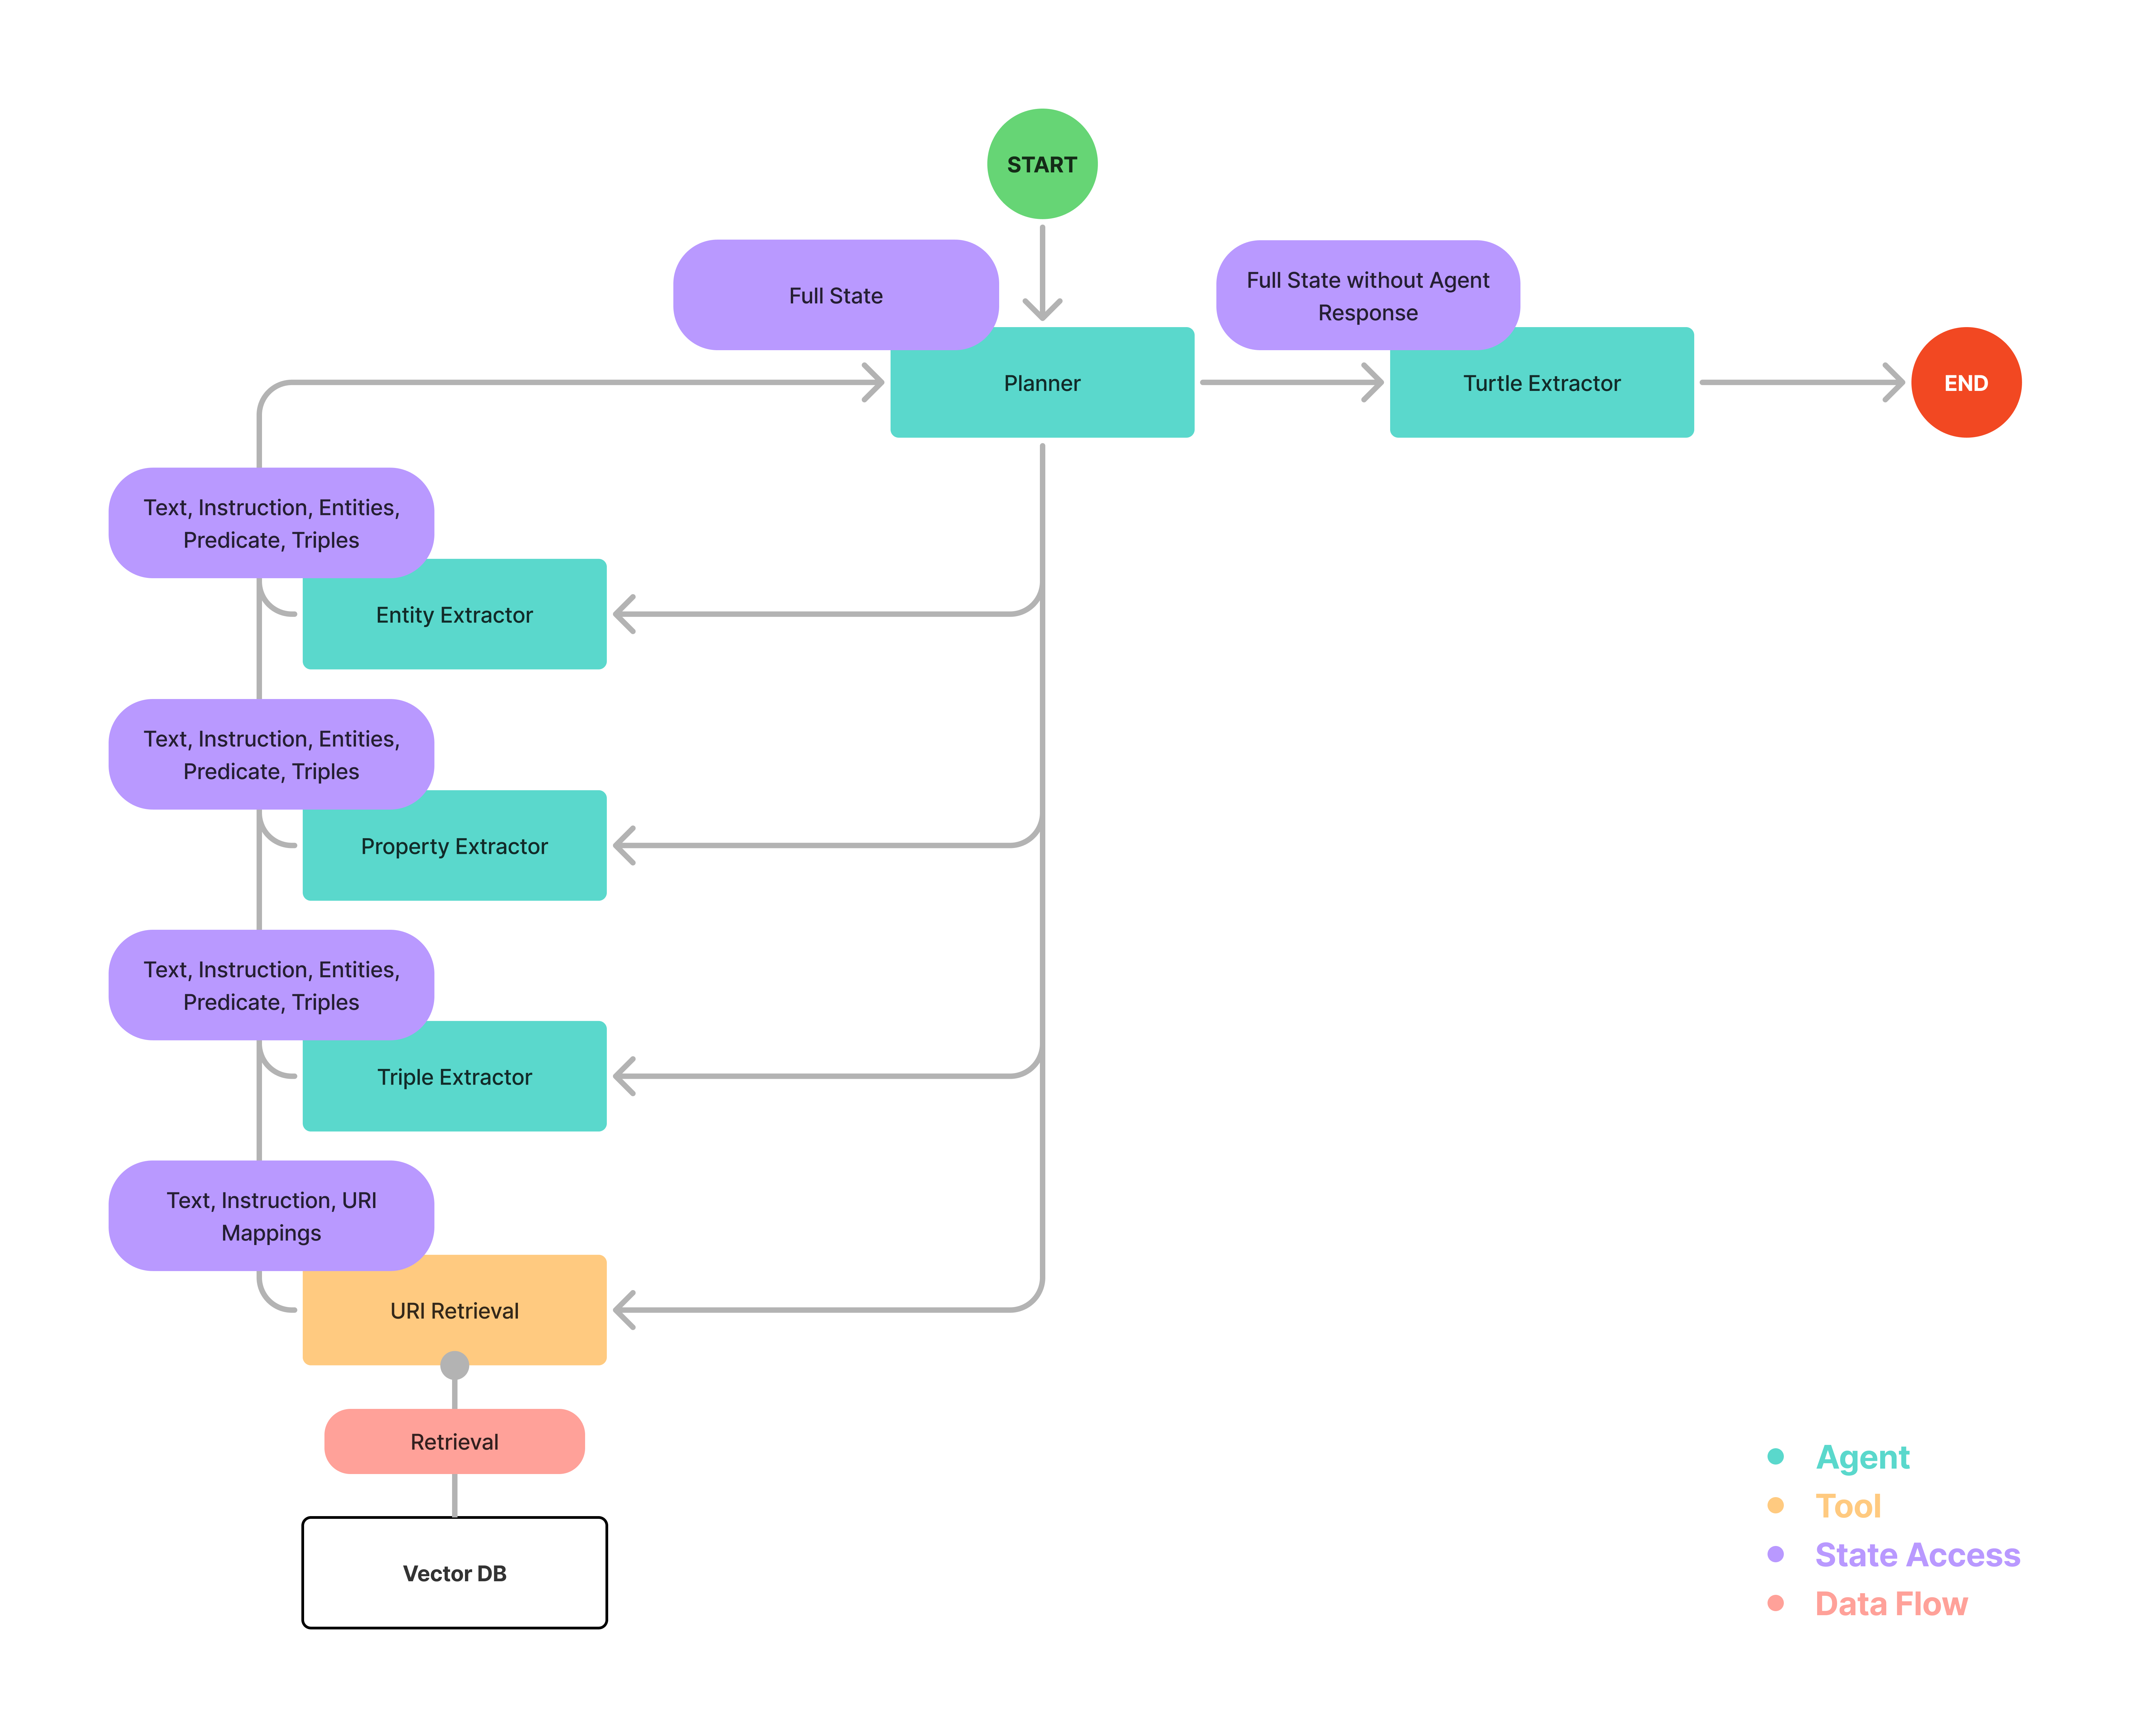
\includegraphics[width=0.7\textwidth]{figures/Simplified Splitted Supervisor Architecture.png}
  \caption[Simplified splitted supervisor architecture showing a streamlined version of the supervisor decomposition with optimized agent interactions]{Simplified splitted supervisor architecture showing a streamlined version of the supervisor decomposition with optimized agent interactions (self-created)}
  \label{fig:simplified_splitted_supervisor_architecture}
\end{figure}

Continuing the principles established in the \textit{Splitted Supervisor Architecture} (\ac{SSA}), the \textit{Simplified Splitted Supervisor Architecture} (\ac{SSSA}) streamlines the agent structure for more efficient interaction and reduced complexity. This design assumes that one agent can still manage all supervision tasks as long as it does not have to generate valid \texttt{turtle} output or operate over an unstructured state. To accommodate this, the architecture retains all specialized agents from the \ac{SSA}, while merging the roles of the \textit{result checker} and \textit{agent instructor} into a single \textit{planner agent}. This agent functions similarly to the original supervisor agent introduced in the \textit{Baseline Architecture}. A more structured and targeted state is introduced to support these adjustments. An overview is provided in Figure~\ref{fig:simplified_splitted_supervisor_architecture}.

A central change of the \ac{SSSA} lies in its redesigned state. Instead of using a general-purpose \texttt{results} field, the state now consists of dedicated fields: \texttt{entities}, \texttt{properties}, \texttt{triples}, and \texttt{uri\_mapping}. Each of these stores the core output of a corresponding specialized agent or tool. This explicit separation enhances transparency and allows the planner agent to access relevant information more directly, without requiring extensive context understanding.

Because this streamlined structure removes access to full agent outputs, a new field named \texttt{agent\_response} is introduced. It captures the raw responses from specialized agents and tools. The planner can inspect these to assess task completion quality, identify errors, or initiate corrective steps. Meanwhile, the \texttt{messages} field is preserved to track dialogue history. In this version of the architecture, it contains only the message history of the planner agent, helping prevent unintended loops.

The actual formation of RDF triples remains delegated to the \textit{Turtle Extractor}, which assembles entities, properties, and URIs into valid \texttt{turtle} syntax. This separation of concerns ensures that the planner agent remains focused on flow control and state refinement, rather than performing complex string transformations.

It should also be noted that the \ac{SSSA} does not incorporate advanced tools such as \textit{semantic validation}, \textit{network traversal}, or the \textit{Turtle-to-Label Converter}. This architectural choice reflects the intention to minimize tool usage and maintain a narrow context footprint for efficient runtime behavior.

This architectural simplification is motivated primarily by practical considerations. As context window limitations increasingly influence \ac{LLM} performance, minimizing unnecessary content in the state becomes essential. At the same time, the system retains the ability to iterate over the \ac{cIE} process when needed. In doing so, the \ac{SSSA} balances agent autonomy with prompt efficiency. It represents a targeted evolution of the supervisor pattern that reduces resource demands while maintaining modular clarity within the multi-agent system.

\subsection{ReAct Architecture}
\label{subsec:react}

\begin{figure}[tp]
  \centering
  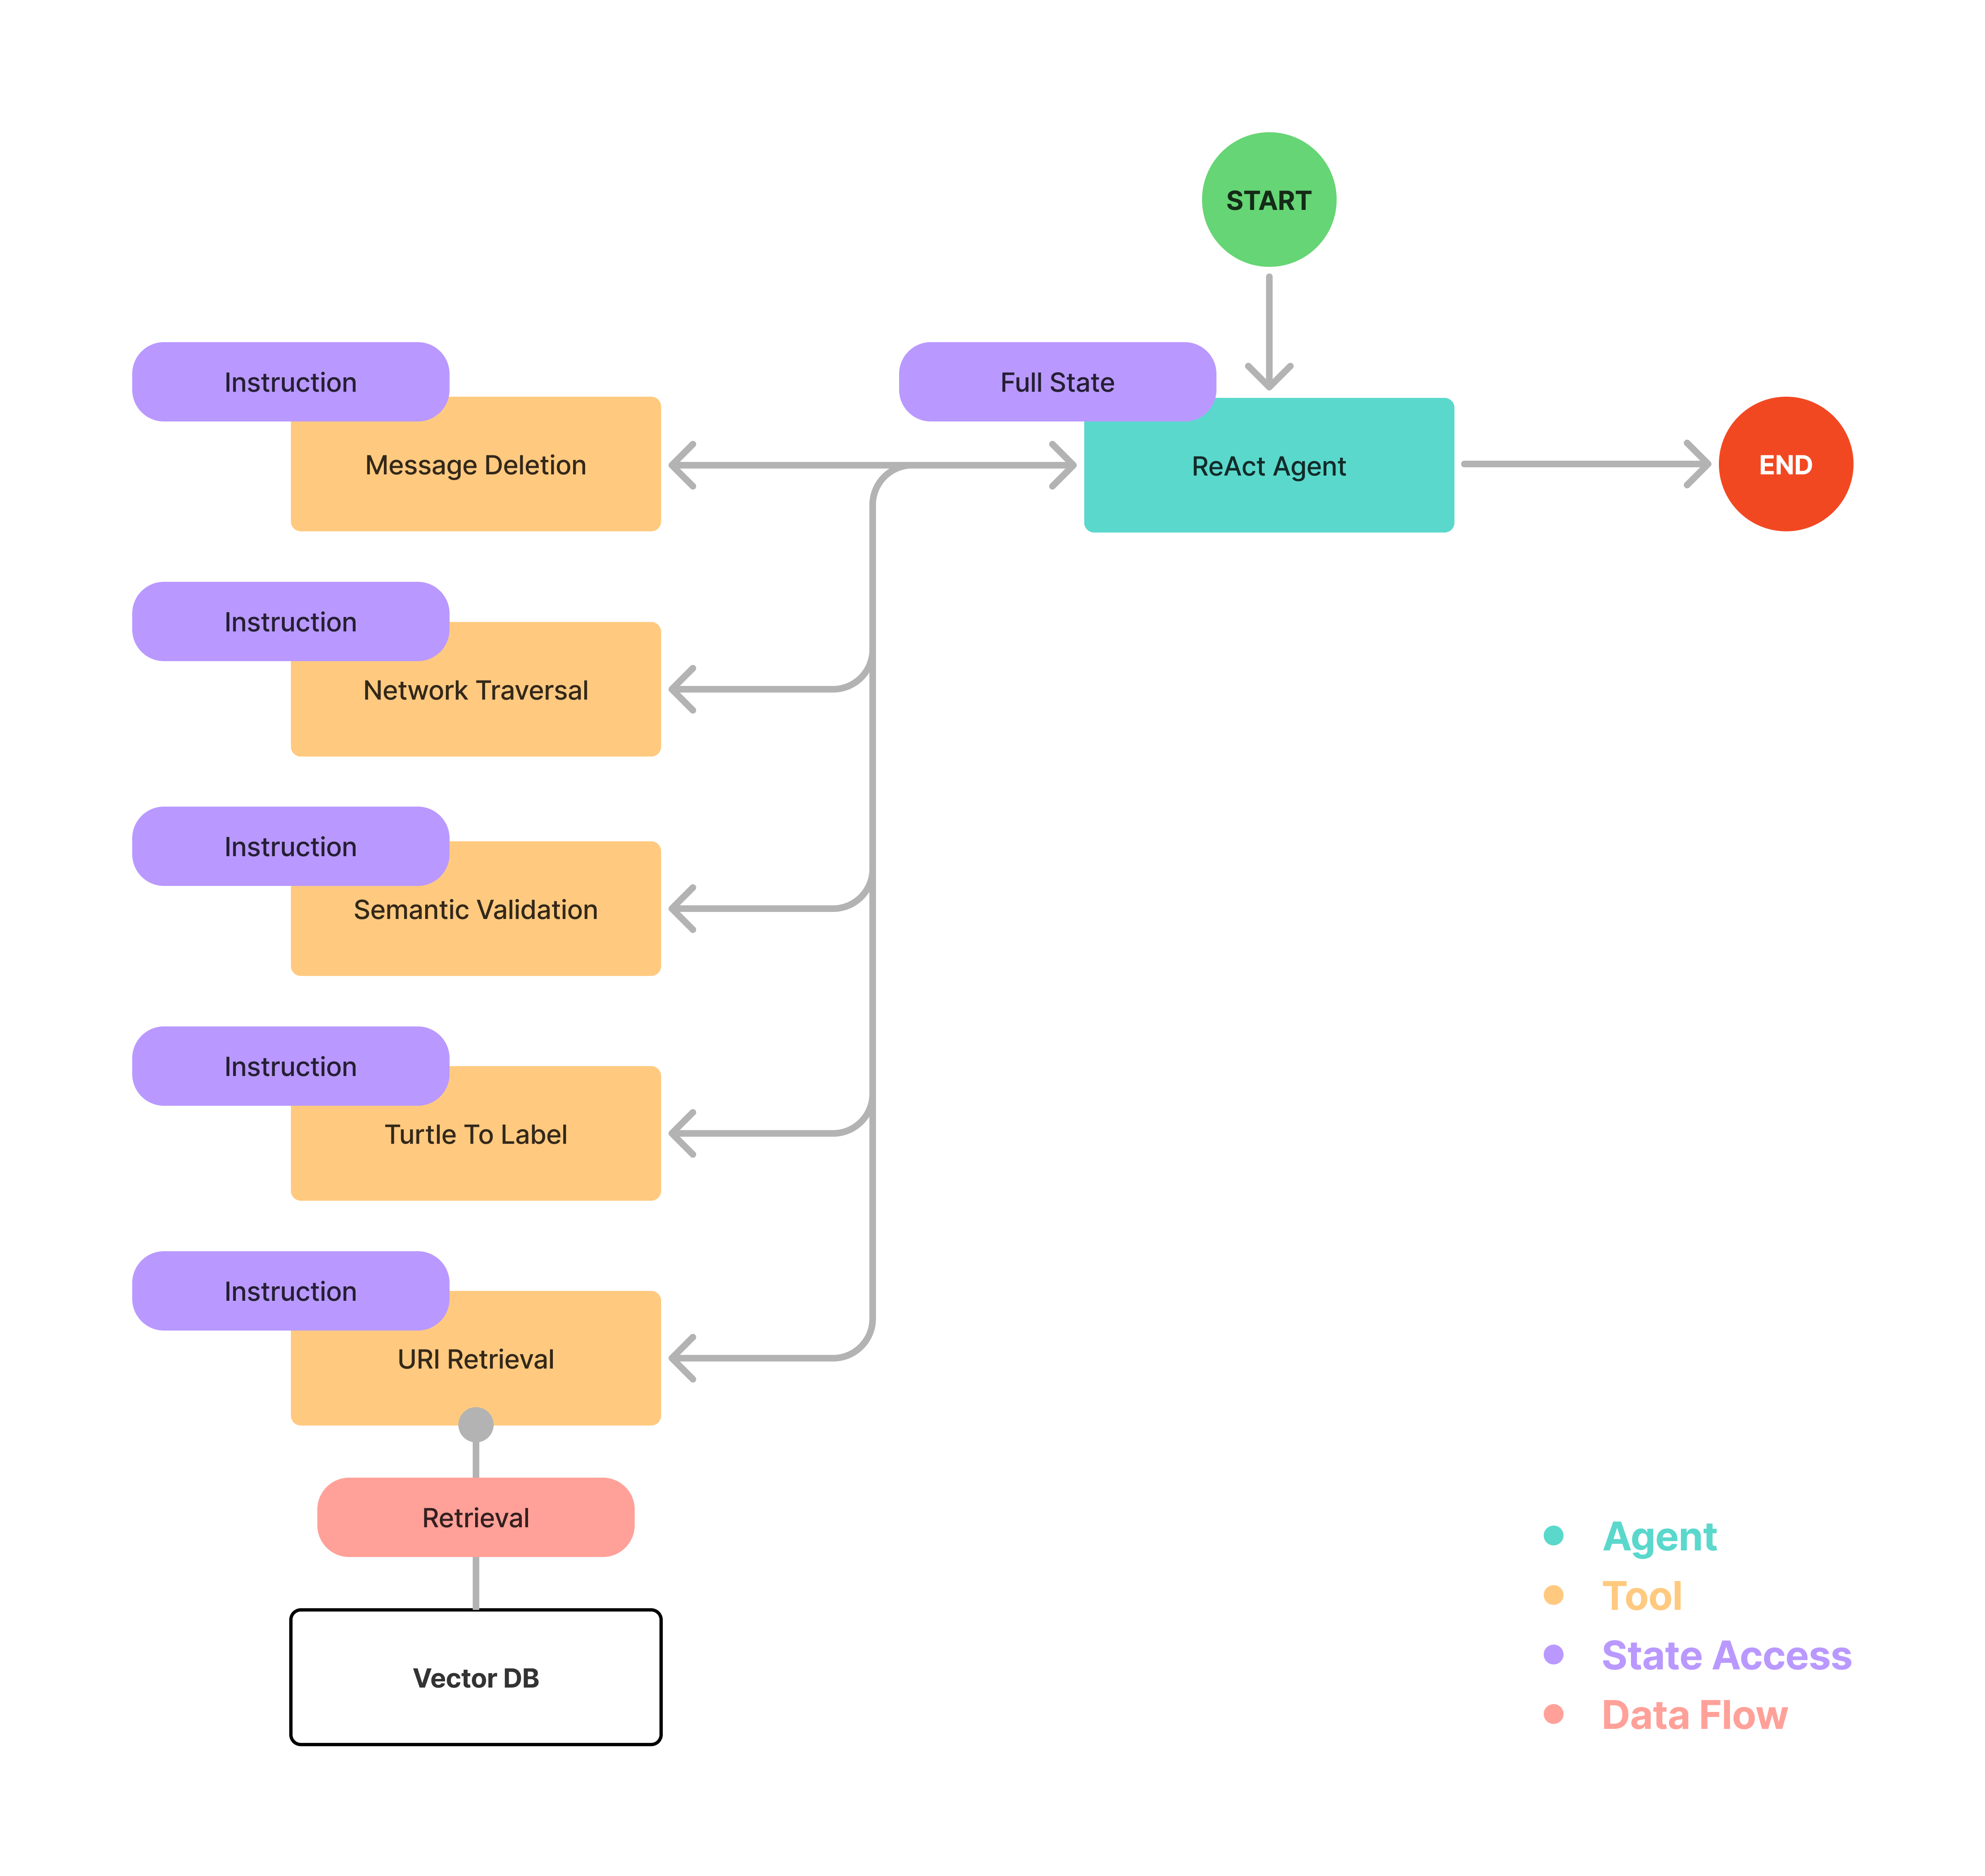
\includegraphics[width=0.7\textwidth]{figures/ReAct Architecture.png}
  \caption[ReAct architecture showing the single-agent approach with reasoning and action capabilities for closed information extraction]{ReAct architecture showing the single-agent approach with reasoning and action capabilities for closed information extraction (self-created)}
  \label{fig:react_architecture}
\end{figure}

Unlike the previously presented solutions, which all rely on a \ac{MAS} to address the complexity of \ac{cIE}, the \textit{ReAct Architecture} takes a contrasting approach. It is designed to evaluate the capabilities of a single agent equipped with reasoning and tool-use abilities. This design choice is based on empirical observations suggesting that simpler configurations can often lead to better results. By eliminating inter-agent communication, the system can focus entirely on tool interactions, reducing coordination overhead and minimizing points of failure.

Another advantage of this joint approach is that it avoids the error propagation typically associated with pipeline-based multi-agent systems. As discussed in Section~\ref{sec:related_approaches}, joint optimization benefits from a single decision point, enabling more coherent outputs. Additionally, reducing the number of agent calls leads to lower inference latency and operational costs.

The state in the \textit{ReAct Architecture} is kept intentionally simple. Since only a single agent is involved, the original baseline structure from Section~\ref{subsec:baseline} is reused. Outputs from tools are written to the \texttt{messages} field, allowing the agent to keep track of prior actions and intermediate results.

To support its reasoning capabilities, the agent is equipped with the \textit{URI Retrieval Tool} from the outset. As the architecture proved effective during iterative evaluations, additional tools were developed to extend its capabilities. These include the \textit{Network Traversal Tool}, the \textit{Semantic Validation Component}, and the \textit{Turtle-to-Label Converter}, each facilitating deeper integration with the underlying knowledge graph. Moreover, a \textit{Message Deletion Tool} was introduced to allow the agent to manage its limited context window by pruning irrelevant or outdated information. The overall tool integration is depicted in Figure~\ref{fig:react_architecture}.

While the \textit{ReAct Architecture} does not qualify as a \ac{MAS}, it plays an important role in contrasting complex \ac{MAS} configurations. It serves as a minimal baseline that demonstrates how much can be achieved with a single reasoning agent. Due to its efficiency and simplicity, it is particularly well-suited for early-stage development and tool testing, making it a logical step within the broader iterative design process. All development steps, including the incremental addition of tools and their evaluated effectiveness, are discussed in detail in Section~\ref{sec:evaluation_configurations}.

\subsection{Network Architecture}
\label{subsec:network}

\begin{figure}[tp]
  \centering
  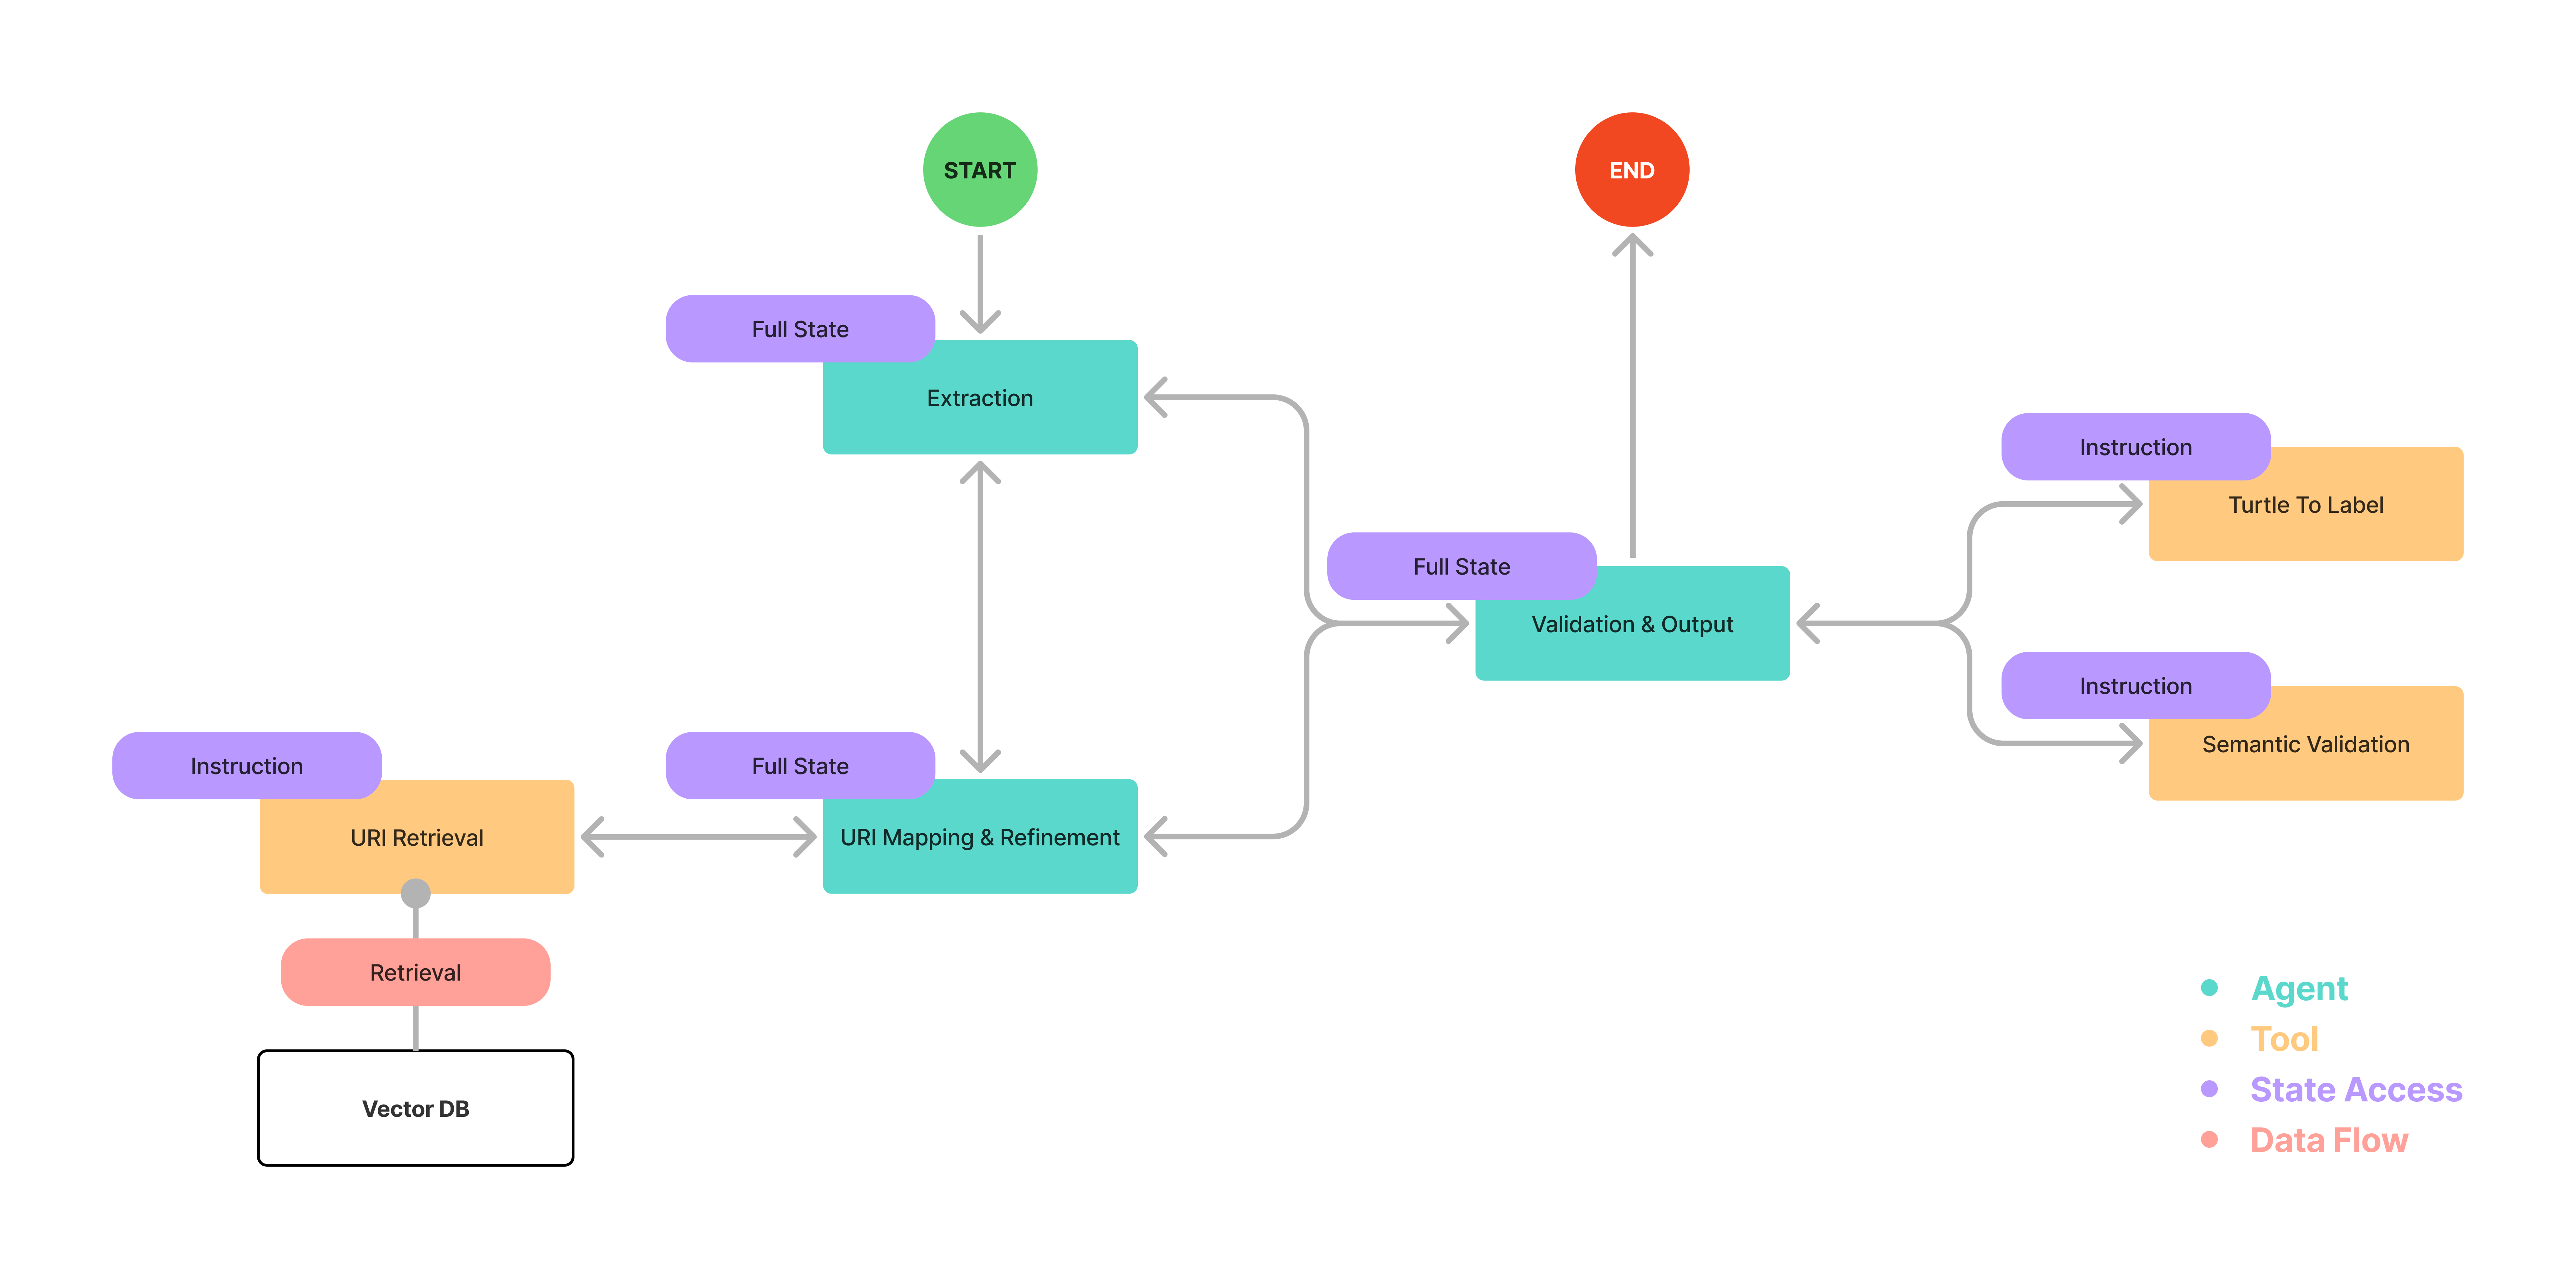
\includegraphics[width=\textwidth]{figures/Network Architecture.png}
  \caption[Network architecture showing the fully connected multi-agent system with dynamic routing and reasoning capabilities]{Network architecture showing the fully connected multi-agent system with dynamic routing and reasoning capabilities (self-created)}
  \label{fig:network_architecture}
\end{figure}

Building on the network pattern introduced in Section~\ref{sec:multi_agent_systems}, the \textit{Network Architecture} represents a culmination of insights gathered from the design and evaluation of all preceding architectures, tools, and state configurations. It aims to combine the reasoning and validation capabilities developed in the \ac{SSA} and \ac{SSSA} with the direct triple extraction process featured in the \textit{ReAct Architecture}. Furthermore, this architecture distributes decision-making across all participating agents rather than centralizing it within a single supervisory entity. An overview of the setup is shown in Figure~\ref{fig:network_architecture}.

The underlying state is an extended variant of the structured design introduced in the \ac{SSSA}. Once again, it prioritizes context-efficient storage of intermediate results. The state fields \texttt{triples} and \texttt{uri\_mapping} are retained, with the latter containing not only the associated URIs but also the original labels of entities or predicates, along with their labels and descriptions retrieved from Wikidata.

To support routing and control logic, a \texttt{call\_trace} is reintroduced. This enables agents to reason over previous interactions and avoid redundant calls. In addition, four further state fields are added: \texttt{last\_call} and \texttt{last\_response} track the most recent invocation and its result; \texttt{agent\_instruction} stores the instruction received by an agent in case it needs to be forwarded across tool calls; and \texttt{tool\_call} holds the most recent tool input. The \texttt{messages} field is also present but differs from other architectures in that it stores the final output string to ensure interoperability with the evaluation framework.

Unlike previous designs, this architecture avoids any state fields that grow cumulatively over time, with the exception of the \texttt{call\_trace}. This constraint reduces context size and forces agents to base their decisions solely on concise result fields and the history of calls. As a result, the system places higher demands on the reliability and precision of agent behavior and may require extensive prompt engineering to ensure consistent performance.

From an agent perspective, the architecture employs three distinct agents with full read access to the complete state. In contrast, tools only receive the input specified in the \texttt{tool\_call} field. Granting agents full-state visibility allows them to make more informed decisions about subsequent actions within the overall flow.

The initial entry point for processing is the \textit{Extractor Agent}, which mirrors the core responsibilities of the main agent in the \textit{ReAct Architecture}, while delegating URI mapping, validation, and Turtle output to separate components. It is the only agent permitted to write to the \texttt{triples} field.

Handling the URI mapping is the responsibility of the \textit{URI Mapping and Refinement Agent}. This agent serves as the central unit for generating and updating URI mappings and is the only component allowed to write to the \texttt{uri\_mapping} field. It is tightly coupled with the output of the \textit{Extractor Agent} and utilizes the \textit{URI Retrieval Tool} to resolve surface forms into structured Wikidata entities and relations.

Validation and formatting are conducted by the \textit{Validation and Output Agent}. This agent prevents hallucination and ensures semantic correctness by validating triples based on features retrieved from the knowledge graph. To do so, it employs both the \textit{Semantic Validation Tool} and the \textit{Turtle-to-Label Converter}. If any extracted triple fails validation, the agent attempts to refine or regenerate it, either by re-engaging the \textit{Extractor Agent} or by forwarding the task to the \textit{URI Mapping and Refinement Agent}, depending on the assumed source of error.

Overall, the network architecture reflects the lessons learned from previous iterations. It omits unpromising tools, makes use of a highly structured and minimal state, and adheres to a fully distributed decision-making strategy. While still grounded in the multi-agent system paradigm, it reduces coordination overhead and context consumption to a minimum.

\section{Agent Tools}
\label{sec:agent_tools}

Agents across the different architectures form the backbone of the approach to \ac{cIE}. However, since \acp{LLM} are inherently limited in their up-to-date knowledge and may hallucinate information, as discussed in Section~\ref{sec:language_models}, additional support is required. Tools serve this purpose by addressing both reliability concerns and performance limitations.

Two general categories of tools are introduced in this work. The first category focuses on integrating knowledge graph information. This includes the \textit{URI Retrieval Tool} (Section~\ref{subsec:uri_retrieval}), the \textit{Network Traversal Tool} (Section~\ref{subsec:network_traversal}), the \textit{Semantic Validation Tool} (Section~\ref{subsec:semantic_validation}), and the \textit{Turtle-to-Label Converter} (Section~\ref{subsec:turtle_to_label}). These tools enable agents to interact with and reason over structured external knowledge.

The second category supports system-level coordination. In this work, only one such tool is introduced: the \textit{Message Deletion Tool} (Section~\ref{subsec:message_deletion}), which is used to manage context size and prevent prompt overflow in long-running agent interactions.

\subsection{URI Retrieval}
\label{subsec:uri_retrieval}

The \textit{URI Retrieval Tool} remains a central component in solving the \ac{cIE} task. While various \ac{LLM}-based agents are capable of extracting free-form triples, the core challenge lies in mapping these triples correctly to the underlying knowledge graph. This mapping capability is provided through the \textit{URI Retrieval Tool}, which enables interaction with the knowledge graph.

Its core function is to receive search terms from the agent and perform similarity-based retrieval using sentence embeddings and cosine similarity. Search terms are generated by the agents, and if a result is not found or deemed unsatisfactory, the agent can adapt the search term, the selected search mode, or the filter setting to repeat the search.
This iterative querying mechanism allows agents to improve mapping performance through controlled retries.

In order to support this mechanism, the tool maintains three search indices, each generated by embedding specific textual representations from the knowledge graph. These include the \texttt{rdfs:label}, the \texttt{rdfs:description}, and example triples, the latter formulated as complete sentences to support semantic encoding of relational context. The construction of these indices is based on Wikidata, the only knowledge graph used throughout this work’s evaluation. The underlying embedding model is consistent across all indices but not central to the approach description at this stage.

The creation of the search indices follows a structured multi-step pipeline. First, documents are loaded from a selected dataset split, such as the test set of the \textit{synthIE dataset}. Second, all entities and properties referenced in these documents are extracted by identifying the URIs of subjects, predicates, and objects. For each subject and object, the corresponding \texttt{rdfs:label} and \texttt{rdfs:description} are retrieved from Wikidata. For each property, in addition to the label and description, an example triple that demonstrates the property’s usage is also retrieved.

In the next step, these textual representations are embedded and stored in separate search indices. The \texttt{rdfs:label} values are embedded into a label index, the \texttt{rdfs:description} values into a description index, and the example triples into an example index. Alongside the embeddings, relevant metadata is stored with each entry. This includes the corresponding URI, the type of the resource (entity or property), the \texttt{rdfs:label} (for entries in the description and example indices), the \texttt{rdfs:description} (for entries in the label and example indices), and the example triple itself (for properties in both the label and description indices).

To control retrieval behavior, the tool interprets two parameters: \textit{search mode} and \textit{filter mode}. The \textit{search mode} selects the semantic space used for similarity retrieval—i.e., whether to search on the labels index, the descriptions index, or the examples index. The \textit{filter mode}, in contrast, restricts retrieval to either entities or properties. This distinction enables more accurate matching and reduces noise, especially when agents provide ambiguous input. In the final iteration, a hybrid retrieval configuration is introduced. It allows label-based retrieval for both entities and properties and example-based search exclusively for properties. Details on these configurations are described in Section~\ref{sec:evaluation_configurations}.

Internally, the \textit{URI Retrieval Tool} parses the agent’s instruction, determines the appropriate search and filter modes per term, and executes a cosine similarity search using the term embedding over the selected index. The top result includes the matching entry’s \texttt{rdfs:label}, \texttt{rdfs:description}, and URI.

Architectures sensitive to context limitations may encounter issues when the tool returns extensive candidate lists. To address this, the tool supports a compact output mode. In this mode, an additional \ac{LLM} call is used to evaluate whether a specific result matches the query. The response is reduced to a simplified URI mapping that includes only the selected URI and a brief justification, omitting alternative matches and detailed descriptions. This compact output is used in configurations of the \textit{Baseline Architecture}, the \ac{SSA}, and the \ac{SSSA}, with the exception of the initial baseline version.

In summary, the \textit{URI Retrieval Tool} equips agents with retrieval-augmented access to structured knowledge. By indexing key components of Wikidata and offering fine-grained retrieval controls, it supports precise URI mapping in a variety of architectures. Its flexibility and accuracy-critical role led to extensive iterations throughout this work, as discussed in Section~\ref{sec:evaluation_configurations}.

\subsection{Network Traversal}
\label{subsec:network_traversal}

The \textit{network traversal tool} represents a further step in incorporating knowledge graph information into the agent workflow. Its main purpose is to support agents in addressing the challenge of selecting appropriate properties, particularly in cases where the input sentence does not contain the exact label of the target property. This issue could lead to the selection of super-properties or sub-properties. By querying structural information from the knowledge graph, the tool enables agents to explore property hierarchies and make more informed decisions.

To achieve this, the tool executes \textit{SPARQL} queries on Wikidata, focusing on the \textit{subproperty of} relation. These queries retrieve both direct super-properties and sub-properties of a given property. To enhance the output's usability, labels are also queried for each retrieved property. Where available, example triples are included for additional context. The resulting output presents the agent with related properties and supporting examples to assess semantic proximity.

An illustrative example can be found in the property hierarchy involving \texttt{member of political party} (\texttt{P102}). This property is a subproperty of \texttt{member of} (\texttt{P463}), which in turn is a subproperty of \texttt{part of} (\texttt{P361}). An agent that extracts a triple such as “Angela Merkel — part of — CDU” might therefore benefit from exploring this hierarchy to identify the most specific and semantically accurate property. The network traversal tool enables this by surfacing both super-properties and sub-properties along with contextual information, such as labels and example triples.

In some cases, individual properties are connected to a large number of related properties, which may result in long and unordered outputs. Since \acp{LLM} often struggle to prioritize relevant information in such cases, additional filtering mechanisms were introduced. Later iterations of the tool included support for inspecting property constraints to assess type compatibility. In Wikidata, these constraints are accessible through qualifiers attached to properties.

Qualifiers in Wikidata are expressed as triples consisting of a predicate and an attribute \cite{Wikidata2025}. For the purpose of this tool, the \textit{property type constraint} is used. This can be further specified as a \textit{subject type constraint} or a \textit{value type constraint}. The actual constraint is represented by the URI of a specific class that the subject or object of a property must conform to.

Using this information, the tool extends its \textit{SPARQL} query to determine whether the subject and object types in a candidate triple align with the constraints of a given property. To increase flexibility, the system allows for one level of abstraction by including the direct superclass of each type. This choice is made to avoid the risk of infinite expansion when traversing class hierarchies, which may occur in unbounded queries against Wikidata.

Through the network traversal tool, agents gain access to structural and semantic context that allows them to refine extracted triples. The tool supports identification of overly broad or overly narrow property selections. However, its usage can introduce considerable overhead due to the potentially large number of returned results. Agents must therefore balance constraint alignment with semantic appropriateness, avoiding overfitting to constraints while maintaining accuracy in property selection.

\subsection{Semantic Validation}
\label{subsec:semantic_validation}

Language models are prone to hallucinations and typically lack the built-in capability to verify their own outputs, as discussed in Sections~\ref{sec:language_models} and~\ref{sec:multi_agent_systems}. To address this limitation, the semantic validation tool was introduced. Similar to the approach used in the network traversal tool, it focuses on type restrictions associated with properties in extracted triples. However, it relies on a pre-filtered, loop-free class hierarchy derived from Wikidata, which allows efficient validation across the full ontology.

The tool receives a complete \texttt{turtle} string as input. This string is parsed and split into individual triples, and each triple is further decomposed into subject, property, and object. As described in Section~\ref{subsec:network_traversal}, qualifiers are then used to determine whether type constraints exist for the subject and object. These constraints are matched against the expected types defined in Wikidata. The output of the tool indicates whether the triple passes validation. In the case of a failed check, the tool also returns the expected subject and object types.

Despite its simplicity, the semantic validation tool provides a valuable mechanism for improving result quality. It helps agents detect cases where a chosen property may be semantically inappropriate, even when descriptions or examples retrieved by the URI retrieval tool appear correct. In this way, the tool serves as a knowledge-aware safety net and provides a foundation for iterative improvement.


\subsection{Turtle to Label}
\label{subsec:turtle_to_label}

Throughout development, agents occasionally produced incorrect URIs due to copy failures or internalized associations from prior knowledge. Given that Wikidata is one of the largest publicly available knowledge graphs, it is likely that parts of it were included in the training data of various \acp{LLM}. As a result, agents may generate URIs based on memorized content rather than verified information. This introduces a particular risk in CIExMAS, where precise usage of \acp{URI} is essential.

Wikidata makes use of a consistent structure across entities, properties, and their relationships. However, it distinguishes between the namespace used to define metadata (such as labels or descriptions) and the one used for actual property assertions. Since other tools in this work, particularly those relying on \textit{SPARQL} queries, depend on correctly defined property URIs, namespace mismatches can lead to tool failures or incorrect results.

To address this issue, the \textit{turtle to label} tool processes the final \texttt{turtle} output and attempts to retrieve the human-readable \texttt{rdfs:label} for each part of every triple. This is done by executing \textit{SPARQL} queries on Wikidata. If a query fails, it typically indicates that the corresponding URI is invalid or refers to an incorrect namespace. In addition to flagging invalid URIs, the tool detects whether a URI exists but lacks an English label, and communicates this to the calling agent.

When hallucinated URIs are generated, the tool highlights these by re-outputting the free-form triples derived from the text, allowing agents to fall back on reasoning over textual content. In doing so, the tool helps expose incorrect or unresolvable references and supports downstream correction.

Overall, the \textit{turtle to label} tool offers a lightweight mechanism for integrating with the knowledge graph and validating agent outputs. Used in tandem with the semantic validation tool, it can strengthen the agent’s ability to detect errors and improves the final quality of extracted triples.

\subsection{Message Deletion}
\label{subsec:message_deletion}

Context bloating has been addressed repeatedly across chapters, particularly through the careful design of agents, states, and tools. An additional strategy introduced in this work is to provide agents with the ability to manage the context proactively. To support this, the \textit{message deletion tool} was implemented.

This tool allows agents to delete individual messages from the state by their identifier. Its development was motivated especially by the needs of the \textit{ReAct Architecture}, where a single \texttt{messages} field stores all outputs from the main agent and tools. Since components such as the \textit{network traversal tool} or the \textit{URI retrieval tool} often produce verbose outputs, this field can quickly become a bottleneck in terms of context size. At the same time, agents are capable of reusing or summarising content. Consequently, the tool enables them to remove outdated or redundant messages and optionally replace them with more concise summaries of the knowledge extracted.

When used alongside agents that can directly edit structured fields, such as the \texttt{triples} field in the \ac{SSSA} or the \textit{network architecture}, this tool supports self-managed context pruning. While this flexibility helps avoid context length limitations entirely, it introduces new challenges for the agents. They must now make reliable decisions about which information to retain, discard, or summarise. The practical implications of using this tool are further discussed in Section~\ref{sec:evaluation_configurations}.

\section{Iterative Prompt Engineering}
\label{sec:iterative_prompt_engineering}

As outlined in Sections~\ref{sec:ai_agents} and~\ref{sec:multi_agent_systems}, \acp{LLM} are highly sensitive to prompt design. Finding suitable prompts is therefore a non-trivial and often challenging task. Since this work focuses primarily on developing a range of multi-agent architectures and demonstrating that knowledge graph incorporation improves performance, the prompt engineering process was conducted manually and iteratively.

The general strategy follows the principles discussed in Section~\ref{sec:agent_design}. Prompts were written and refined to be solvable by a human, aiming to leverage the reasoning capabilities of \acp{LLM} without exceeding their limitations. In addition, most prompts include examples to support \textit{in-context learning}. Depending on the use case, these examples either illustrate tool instructions or are drawn directly from the dataset used in a specific task, such as entity extraction. In the latter case, original text passages were combined with the expected entities to show the agent which types of triples are considered relevant.

Another technique applied throughout this process is guided \ac{CoT}. Agents were explicitly instructed to follow a predefined and prompted chain of thought. Most prompts consist of a consistent structure, including a role introduction, a description of available tools (if applicable), a list of guidelines, illustrative examples, and finally the input state. The guidelines serve to handle edge cases and known failure modes, whereas the role introduction typically remains unchanged across different prompt iterations.

As discussed in Section~\ref{sec:agent_design}, clear tool descriptions are essential to enable proper tool usage. In CIExMAS, tools are embedded directly in the prompt. Each is presented with an identifier, a name, and a descriptive text. This description also defines the expected instruction format. This is particularly relevant for tools such as the URI retrieval component, where specific search and filter modes must be communicated to the agent through the prompt.

In summary, prompt engineering in CIExMAS is realized as a manual, iterative process. The design principles are aligned with best practices observed in prior research, emphasizing human-readability, structured layout, and the inclusion of well-selected examples—either for tool usage or for solving the core extraction tasks.

\section{Error Handling}
\label{sec:error_incorportion}

As \acp{LLM} are designed to generate unstructured text, problems can arise when a specific output format or the use of predefined tags is expected. One solution lies in leveraging the reasoning and looping capabilities of agent systems to incorporate error messages into the agentic flow. This allows agents to detect and potentially correct faulty behavior, particularly when error messages are well-defined and understandable.

As described in Section~\ref{subsec:baseline}, the consistent parsing strategy across CIExMAS is the use of XML tags to mark key elements in agent responses, such as the identifier of the next agent or the corresponding instruction. Therefore, each agent is prompted to return information in an XML-tagged format, which is subsequently parsed during execution. For example, the agent output is scanned for a \texttt{<goto>} tag to determine which agent or tool should be called next. Similarly, the \texttt{<instruction>} tag is used to extract task-specific input. These parsing routines are vulnerable to failures if tags are missing, malformed, or empty.

To manage such failures, all parsing steps in the agent execution loop are enclosed in \texttt{try}-\texttt{except} blocks. If an expected tag is not found or cannot be interpreted correctly, the system generates a specific error message describing the missing or malformed element. This error is then returned to the calling agent, allowing it to revise its output in the next reasoning step.

Similar mechanisms are implemented for tool inputs. If an agent provides a malformed instruction, such as an undefined search mode for the URI retrieval tool, the tool parser triggers an exception and returns a descriptive error message back to the agent. This enables iterative corrections without terminating the execution.

Another source of errors involves incorrect or hallucinated agent outputs. As discussed in Sections~\ref{subsec:semantic_validation} and~\ref{subsec:turtle_to_label}, dedicated tools are used to validate the semantic and syntactic correctness of extracted triples and URIs. In the final execution step, all generated Turtle outputs are parsed using a Turtle parser to verify compliance with syntax rules. Errors at this stage include undefined prefixes, incorrect namespaces, or invalid characters. These issues are again transformed into structured error messages that can be interpreted by the system.

Through this layered error handling, CIExMAS can detect and respond to a broad range of issues—from missing XML tags to malformed Turtle syntax. Error messages are returned in a machine-readable format and reintegrated into the agent flow, enabling agents to revise and repeat failed steps. External issues such as context overflows or GPU memory errors remain outside the scope of this system-level handling. Nevertheless, within the agentic loop, this approach increases robustness and helps ensure that a valid output can be generated for each datapoint.

\chapter{Evaluation}
\label{ch:evaluation}

This chapter is about the overall evaluation of the effectiveness of multi-agent system in doing \ac{cIE}. In general, the multi-agent system was build using python. The overall setup of it including the used datasets and Wikidata incorporation, the used language models and used frameworks will be explained in section \ref{sec:evaluation_setup}. Furthermore, the calculation of the evaluation metrics which are used for the comparison later will be outlined in section \ref{sec:evaluation_metrics}. The results within this evaluation will be done in section \ref{sec:evaluation_configurations} leading by an overview comparison of the best CIExMAS configuration to the approaches synthIE \cite{Josifoski2023} and GenIE \cite{Josifoski2021} on the a split of the synthIE dataset \cite{Josifoski2023}. This will be followed by the single interation steps and their results. In section \ref{sec:discussion} all results will be concluded and interpreted.

\section{Evaluation Setup}
\label{sec:evaluation_setup}

The evaluation setup consists out of three essential parts. First, is the subsection \ref{sec:dataset} about the dataset used for the evaluation and espeically which split of it is used. Additionally, the subsection contains details about where external information are stored for the information. Afterwards the language models and providers will be outlined in subsection \ref{subsec:eval_language_models}. The evaluation setup will be concluded by section \ref{sec:evaluation_setup} about the concrete agentic framework used. In addition, huge parts of the work is traced using the open-source application LangFuse \footnote{available under \url{https://langfuse.com}}.

\subsection{Dataset and Comparison Models}
\label{sec:dataset}

The evaluation is based on the dataset synthIE, with one experiment conduct using REBEL. Both datasets, which are described in section \ref{sec:related_datasets}, contain triples, that are extracted out of a given text. Each extracted triples contains unique identifiers from Wikidata for each part of the triple, which make them ideal for \ac{cIE}. Each identifier could be resolved within the entity namespace \texttt{https://www.wikidata.org/entity/}.

Both datasets follow a similar structure. Both datasets are stored in json lines, which is a line separated format of objects consisting of entities, relations and triples. Each entity and relation, which can also be named as property, is further split down into a surfaceform and uri, which is a unique identifier. The surfaceform is exactly how the entities and relations are written in the given text. The uri field is the local part of the Wikidata Qname. A Qname itself has a prefix, which is the namespace in the case of Wikidata, and a local part which is the unique identifier \cite{ASF2010}. This means that the uri field is for instance Q120 with the surfaceform \enquote{June}. The full entity \enquote{June} can only be detected in the namespace of \texttt{https://www.wikidata.org/entity/}. The triples contain of a subject, object and predicate, which itself are build up like entities and relations.

As already outlined in section \ref{sec:related_datasets} there are two datasets of synthIE, which are synthIE-code and synthIE-text. Both versions of the datasets differ in the GPT-3.5 model used for the text generation. As the text model showed better performances, the evaluation is strictly done on synthIE-text.

Nevertheless, all evaluation configurations until section \ref{subsec:knowledge_graph_integration} were developed on synthIE-code, as of the larger amount of training data could have provided are more extensive development set in order to detect as much edge cases as possible. For development reasons, the train-split of synthIE-code was used for those configuration and sorted, so that the document with id one is the first in the jsonlines file.

As of upcoming limitations due to dataset quality and the experience of developing on at most ten examples, the latest developments were done on the validation-split of synthIE-text, which is also sorted and includes the same underlying triples but different text. The validation split is used, as synthIE-text does not offer a train split. In the end, this offers a higher quality of text and might produce more solvable edge cases, than triples that are hard to find in the text.

The evaluation was done for all comparison models and evaluation configrations of CIExMAS on the first 50 documents within the sorted test split of the synthIE-text datasplit. The number was choosen based on limitation in computing capacities, especially for agent call intense architectures like \ac{SSA} or \ac{SSSA}. Again synthIE-text was choosen, as it was perceived by \citet{Josifoski2023} to produce improved results in comparison with synthIE-code without changing the training dataset, which implies a higher dataset quality. In addition, the experiments have shown a more detectable result of triples.

To illustrate the distinction between \texttt{synthIE-code} and \texttt{synthIE-text}, the first document of both datasets is shown in the following example. In the \texttt{synthIE-code} version, the sentence reads: "\emph{'Groovin' Blue' is an album by Curtis Amy, released on Pacific Jazz Records.}" In contrast, the \texttt{synthIE-text} version presents a variation: "\emph{Groovin' Blue was released on Pacific Jazz Records and performed by Curtis Amy.}" While both versions encode the same structured triplets, which can be found in table \ref{tab:triple-example}, the textual surface varies. The synthIE-text version already gives a hint on the exact property, which in the case of synthIE-code is harder to find.

\begin{table}[h]
  \centering
  \begin{tabular}{l l l}
    \toprule
    \textbf{Subject} & \textbf{Property} & \textbf{Object}        \\
    \midrule
    Groovin\_Blue    & record label      & Pacific\_Jazz\_Records \\
    Groovin\_Blue    & performer         & Curtis\_Amy            \\
    \bottomrule
  \end{tabular}
  \caption{Surfaceform Triplets - DocID: 0 - synthIE Code \& Text}
  \label{tab:triple-example}
\end{table}

As it was planned to benchmark the best CIExMAS models on the REBEL dataset, the first 50 samples in the sorted test-split were uploaded in the vector databases. Like already outline, CIExMAS focussed mainly on synthIE as foundation for developing the agents, which could conclude in worse results on REBEL. As of testing, no approach scored over 0.1 F1-score, which is why REBEL was not further used for evaluation. The results of the testing can be found in the section \ref{sec:rebel_testing} of the appendix.

Both datasets were evaluated on various different models before. Espeically for the synthIE dataset, the solutions of \citet{Josifoski2023} synthIE- and GenIE were used as they were used pre-trained under \url{https://github.com/epfl-dlab/SynthIE}. For the synthIE solution all three versions synthIE$_{T5-base}$, synthIE$_{T5-base-SC}$ and synthIE$_{T5-large}$ were evaluated. For the GenIE solution the version GenIE$_{T5-base}$ and GenIE$_{T5-base-SC}$ were tested. The abbreviation \textit{SC} stands for subject-collapsed, which means, that those variants outputs subject grouped triples. All models are using the Flan-T5 \ac{LM}. Like the CIExMAS solution, those solutions were also evaluated against the same samples of synthIE-text.

In the end the REBEL dataset showed very low scores on testing on the best models like depicted in the appendix \ref{sec:rebel_testing}. To provide an example of the data quality, in the following sentence \enquote{Richard H. Weisberg is a professor of constitutional law at the Cardozo School of Law at Yeshiva University in New York City, a leading scholar on law and literature.}, the two triples \textit{(Cardozo School of Law; headquarters location; New York City)} and \textit{(Yeshiva University; located in the administrative territorial entity; New York City)} are expected. This is just a very small subset of triples, that could be derived from the text. In addition, many texts are spreading across two paragraphs, making the \ac{cIE} task harder. As the scores were below 0.1 F1 for the triple extraction and the triple quality in this test set can be found below what is human extractable, it was decided to not further proceed with an REBEL optimisation.

Overall the first 50-sample sorted synthIE-text dataset serves as benchmark for CIExMAS and comparison models. In addition, the dataset can also show which evaluation configuration changes had which impact on the overall performance.

\subsection{Knowledge Graph Access}

Like outlined in various sections about knowledge graph incorporation tool in section \ref{sec:agent_tools} it is necessary to provide the agent system direct access to Wikidata as underlying knowledge graph. To provide faster latency this is done by a system consisting of Qdrant as vector database, Redis as key-value storage and Apache Jena Fuseki as local SPARQL endpoint. All of this is hosted on a virtual private server, which provide lower latency than using the SPARQL endpoint of Wikidata directly. Nevertheless, a direct access to the Wikidata SPARQL endpoint is used in the network traversal and turtle to label tool to get the restrictions directly.

The URI retrieval tool, like already outlined in the corresponding subsection \ref{subsec:uri_retrieval}, needs a search index to produce relevant mappings. In this evaluation each search index is one collection in the hosted Qdrant vector storage. It has to be mentioned, that using some kind of database that supports similarity search was necessary to support the outlined approach.

In order to fill the Qdrant collections, the relevant data was pre-collected for all development and benchmarking datasets and their corresponding samples. This means that also when developing and benchmarking on synthIE dataset, the benchmarking parts of REBEL, meaning entities and properties are indexed in all collections of Wikidata. This is based on the goal to make CIExMAS real-world ready, where it would have to decide out of the whole underlying knowledge graph, while keeping the collections manageable. On the otherside, this enabled a simple dataset switch in either development or benchmarking.

As already stated, the semantic validation needed a loop-free hierarchy graph of the entities and properties of Wikidata. To provide them across various machines, a instance of Apache Jena Fuseki was hosted with a class- and a property-hierarchy. As those graphs were also smaller, this gave another performance boost over calling the SPARQL-endpoint of Wikidata directly.

The key-value store Redis is used for faster data processing pipelines and debugging. This means, that the redis primarily stores, which data from Wikidata have already been stored into the Qdrant database. Alongside it also stores the label, the description and the type of element saved from Wikidata, so that also the displaying the labels is faster. Displaying labels faster also saves time, when for instance benchmark runs have to be evaluated in detail and each URI must be transformed into a human-readable label.

Overall the usage of a vector store is necessary to solve the task of \ac{cIE} with the CIExMAS approach. Furthermore, things like a triple store and a key-value store can help to make information available across multiple machines and decrease latency. Combined this enables the overhead of preparing and executing of the agent system to be low.

\subsection{Language Models}
\label{subsec:eval_language_models}

The choice of a language model is a very complex task in regards of a multi-agent system. For such a task, the \ac{LLM} has to be able to follow prompts, plan, reason about tasks, but also have to extract triples and know how knowledge graphs triples are typically build. In addition, from the kick-off of the CIExMAS project until the end multiple models have been published. Those models were also not tested before on the related approaches to CIExMAS, which lets the evaluation start at the foundation.

An additional limitation is the system used to benchmark as well as the providers used to develop the system. The benchmarks were all executed on 2x Nvidia A100 with 48GB VRAM, which had to run the \ac{LLM} using vLLM \footnote{available under \url{https://docs.vllm.ai/en/latest/}} and the embedding model using Ollama \footnote{available under \url{https://ollama.com}}. Therefore, the \ac{LLM} parameter limit was experienced at circa 70 billion parameters for a 4-bit quantised \ac{LLM}. In addition, the extensive development and evaluation was limited to open source models, as of the traceability of CIExMAS and to offer more flexibility in model use. Additionally, the evaluation could be done on local servers instead of using credits at AI vendors for the token instense benchmarking.

In the course of the work, Llama 3.3 70B showed the best performance in the outlined capabilities, especially in executing a multi-agent system and following instructions. That is why all benchmarks of CIExMAS except for the model variation were done on a 4-bit AWQ model of Llama 3.3 70B named \texttt{kosbu/Llama-3.3-70B-Instruct-AWQ}. The high performance also matches with the benchmarks executed by \citet{Meta2024}, which showed a similar performance to GPT-4o or Claude 3.5-Sonnet, which were state-of-the-art models back at the time, but needed more parameters and are no open sourced. The Llama 3 Series furthermore is build like the GPT models, but could leverage a large scale of high quality data, which reduced the parameter size down to 405 billion parameters in Llama 3 and 70 billion parameters in Llama 3.3, while keeping the performance up \cite{Grattafiori2024,Meta2024}.

More recently Google released a new open source model called Gemma3 which got ranked one of the best models on the human-evaluated LMSys Chatbot Arena \cite{Chiang2024}, while maintaining a low number of 27 billion parameters \cite{Team2025}. Nevertheless it showed slightly lower scores than Llama 3.3 70B in for instance the MMLU-Pro benchmark. Furthermore, the Gemma3 model showed shortcomings in instruction following and executing a logic agent flow.

In addition, newer model architectures like Mixture-of-Experts or reasoning models became present with the rise of Deepseek-R1 or the Meta Llama 4 models \cite{DeepSeekAI2025,MetaAI2025}. Those models have also shown high benchmarking results, while keeping the parameters lower then top-end state-of-the-art models. Those models partly have shown higher performances, but as the reasoning capability keeps looping over the LLM and produces a higher need for tokens as well as higher needs on resources, those models were not used for development due to hardware and time limitations.

Nevertheless both Gemma3 and Meta Llama 4 are used to test different models with the best evaluation configuration of CIExMAS. Therefore, the whole configuration stayed the same. This can lead to expositions of the prompt senstivity of the other models, which can show underperformance in comparison to a perfectly adapted prompt. In order to use Gemma3 on the given setup, a 4-bit GPTQ-quantised version named \texttt{ISTA-DASLab/gemma-3-27b-it-GPTQ-4b-128g} was used. As the best version at the time is Llama 4 Maverick and this model requires over 96GB of VRAM, that the two available Nvidia A100 GPUs offer, the evaluation on Llama 4 Maverick was done on SambaNova Cloud, which is a provider for LLM inference.

All in all, Llama 3.3 70B remained the ideal model for fast development using SambaNova Cloud and the unquantised Llama 3.3 70B model, while the main evaluation was done on the quantised model. This model already provided a great leap over the previous used \ac{LM} of \citet{Josifoski2023}. Therefore, the model advance are included in CIExMAS. To test even more recent advances, other models were also included in the evaluation.

\subsection{Agentic Framework}
\label{subsec:agentic_framework}
In order to evaluate any agentic system, an agentic framework is needed. As the \ac{LM} and the embedding model run on vLLM and Ollama, while the \acp{LLM} in development are called from cloud providers, the agentic framework is also required to support those requirements. In addition it needed to support custom states like outlined in chapter \ref{ch:approach}.
A package that supported those requirements and had the flexibility to be extended was LangGraph like already stated in section \ref{sec:multi_agent_systems}. As LangGraph implements mainly flow features, but in the form used does not interact with the \acp{LLM} directly, the \ac{LLM} and embedding model access were again flexible. The decision was taken on LangChain, as LangGraph and LangChain were integrated into each other. Therefore, the monitoring using Langfuse can be done seemlessly on the agent overview level. This gives the outlined capability of agent tracibility outlined in section \ref{sec:agent_design}. Another advantage of LangChain is the wide availability of adapters to various LLM providers. In addition, all frameworks are also open-sourced projects and have big communities what was supporting the creation of CIExMAS.
In the end, many agentic and \ac{LLM}-frameworks in general could be used. Nevertheless, the combination out of LangChain, LangGraph and Langfuse was taken due to their match in requirements and wide-spread usage in the community. With those tools, the best practises of agent design are enabled for the implementation of CIExMAS.

\section{Evaluation Metrics}
\label{sec:evaluation_metrics}
The evaluation metrics are crucial to make CIExMAS comparable to other models, but also to identify optimisation potentials in CIExMAS. The evaluation is therefore based on evaluation metrics proposed by \citet{Josifoski2021}, which are meant to define true and false positive triples. Derived from defining positive and negative matches, typical score like F1-score, precision or recall can be defined. In addition to \citet{Josifoski2021} we propose a definition of close matches.

To define close matches, it is important to outline the definition of a match proposed by \citet{Josifoski2021}. Therefore, the set of predicted and actual triples are compared per document. A predicted triple is a match, when there is a triple in the set of actual triples per document, where each part of the triple matches by its \ac{URI}. Derived from this, there can be a number of matching triples, so called true positive triples be derived. All remaining triples are false positive triples. All unmatched triples of the actual triple set are then false negative triples.

In addition to the main category triples proposed by \citet{Josifoski2021}, four additional categories for direct matches were derived: Subject, Property, Object and Entity. This has the background of showing where a configuration lacks off capability. In addition, it shows which configuration can handle each part the best and then offers a insight to derive prompts to other configurations. Entities in this case is a set of all subject and objects in a document, where the place in the triple does not matter. The metric is calculated in the same way for those addition categories like for the triples.

To offer insights in how close the predictions are towards the expected results, soft matches are addition proposed for the property. Those soft matches also includes triples that use a super-property of the expected property as true positive. This matches are defined as parental soft matches. When a predicted property is either a super- or sub-property of the expected property, the match is defined as related soft match. Both soft match categories can be applied to either the predicate and the triple category.

Those soft matches are implemented by using a greedy search, whether a triple matches a triple from the gold standard and vice a versa to detect to correct number of true and false positive as well as false negative triples. This opens the error of creating f1-scores, precision and recalls over one, as multiple triples of the predicted set could match to one triple in the gold standard. That is why the recall is calculated as number of gold standard triples or properties that were detected devided by the total number of gold standard triples, while the precision was done the same but on prediction side. This follows also the common definition of precision and recall precisely.

The pre-liminary evaluation metrics of true positive, false positive and false negative triples, subjects, properties, objects and entities as well as the related soft matches are calculated for each document. In addition with the resulting turtle string they are saved into a excel sheet, which later on can be processed to F1-scores, precisions and recalls. As the scores are evaluated document-wise, an overall macro or micro average can be used for all three scores. In the following evaluation macro-scores are used, when the averaging method is not further defined, as the macro average gives each document equal weight regardless of the amount of triples in each document.

To illustrate how the evaluation metrics are computed, we consider a concise toy scenario with three triples about Angela Merkel.  Two sets are contrasted below: the triples predicted by CIExMAS and the manually curated gold standard.  Because the example is deliberately minimal, every intermediate step—from strict matching to soft matching—can be verified by hand.

\begin{table}[ht]
  \centering
  \label{tab:merkel_triples}
  \begin{tabular}{p{0.46\textwidth}p{0.46\textwidth}}
    \toprule
    \textbf{Predicted triple} & \textbf{Actual triple}                                      \\ \midrule
    Angela~Merkel ; \textit{profession} ; Politician
                              & Angela~Merkel ; \textit{profession} ; Politician            \\[0.2em]
    Angela~Merkel ; \textit{is~member~of} ; CDU
                              & Angela~Merkel ; \textit{is~member~of~political~party} ; CDU \\[0.2em]
    Angela~Merkel ; \textit{hobby} ; Tennis
                              & Angela~Merkel ; \textit{lives~in} ; Berlin                  \\
    \bottomrule
  \end{tabular}
  \caption{Predicted versus actual triples for Angela~Merkel.}
\end{table}

In this ontology the predicate \textit{is~member~of~political~party} is a declared sub-property of the more general predicate \textit{is~member~of}.  Consequently, when CIExMAS predicts \textit{is~member~of} while the reference solution specifies the specialised variant, the pair is counted as both a \emph{parental soft match} (because the prediction is a direct super-property) and a \emph{related soft match} (because "related" embraces any super- or sub-property relationship).  Such soft matching awards partial credit whenever predicted and gold predicates are ontologically linked, even if their URIs differ.

\begin{table}[ht]
  \centering
  \label{tab:merkel_metrics}
  \begin{tabular}{lrrrrrr}
    \toprule
    Category               & TP & FP & FN & Precision & Recall & $F_1$ \\ \midrule
    Triples                & 1  & 2  & 2  & 0.33      & 0.33   & 0.33  \\
    Triples -- Parental    & 2  & 1  & 1  & 0.67      & 0.67   & 0.67  \\
    Triples -- Related     & 2  & 1  & 1  & 0.67      & 0.67   & 0.67  \\
    Subjects               & 1  & 0  & 0  & 1.00      & 1.00   & 1.00  \\
    Properties             & 1  & 2  & 2  & 0.33      & 0.33   & 0.33  \\
    Properties -- Parental & 2  & 1  & 1  & 0.67      & 0.67   & 0.67  \\
    Properties -- Related  & 2  & 1  & 1  & 0.67      & 0.67   & 0.67  \\
    Objects                & 2  & 1  & 1  & 0.67      & 0.67   & 0.67  \\
    Entities               & 3  & 1  & 1  & 0.75      & 0.75   & 0.75  \\
    \bottomrule
  \end{tabular}
  \caption{Per--category evaluation metrics for the example in Table~\ref{tab:merkel_triples}.  "Parental" and "Related" rows count soft matches where the predicted predicate is, respectively, a super-property or any super/sub-property of the expected predicate.}
\end{table}

The strict comparison in Table~\ref{tab:merkel_metrics} yields one fully correct triple, perfect subject recognition, and largely accurate object selection, while property alignment remains the principal source of error.  Allowing parental and related soft matches mitigates this deficiency by recognising the semantic proximity between \textit{is~member~of} and \textit{is~member~of~political~party}.  For example, in the object category two true positives, one false positive, and one false negative produce a precision and recall of $\tfrac{2}{3}$, resulting in $F_1\approx0.67$.  The same arithmetic is applied uniformly across all other categories.

Because these metrics are computed on a document-by-document basis, macro averages give each document equal weight, thereby yielding an interpretable, document-equitable overall score.  Evaluating at multiple granularities—triples, subjects, predicates, objects, and undifferentiated entities—while incorporating soft matches ultimately offers a robust foundation for diagnosing and improving CIExMAS.



\section{Evaluation Overview}
\label{sec:evaluation_overview}

\begin{table}[h]
  \centering
  \begin{tabular}{l|rrrrr}
    \toprule
    \textbf{Model}         & \multicolumn{5}{c}{\textit{\textbf{Triples}}}                                                                     \\
                           & Precision                                     & Recall         & F1             & Parental F1    & Related F1     \\
    \midrule
    synthIE$_{T5-large}$   & \textbf{0.835}                                & \textbf{0.832} & \textbf{0.831} & \textbf{0.841} & \textbf{0.858} \\
    synthIE$_{T5-base-SC}$ & 0.789                                         & 0.798          & 0.789          & 0.819          & 0.833          \\
    synthIE$_{T5-base}$    & 0.784                                         & 0.769          & 0.775          & 0.812          & 0.826          \\
    GenIE$_{T5-base}$      & 0.527                                         & 0.344          & 0.391          & 0.406          & 0.419          \\
    GenIE$_{T5-base-SC}$   & 0.527                                         & 0.320          & 0.372          & 0.391          & 0.404          \\
    \midrule
    \textbf{CIExMAS}       & 0.728                                         & 0.635          & 0.665          & 0.728          & 0.728          \\
    \bottomrule
  \end{tabular}
  \caption{Performance comparison of CIExMAS against state-of-the-art models on the synthIE dataset.}
  \label{tab:evaluation_overview}
\end{table}

The best CIExMAS configuration tested on the outlined 50-sample synthIE-text dataset, was found using the network architecture outlined in section \ref{subsec:network}. The exact configuration can be found in section \ref{subsec:full_network_agent_architecture}. The configuration scored 62\% F1 better than the best GenIE solution of \citet{Josifoski2021} and reached near performance to the synthIE models with the largest performance gap being 25\% of F1 increase. All models were evaluated on the same dataset samples.

In total the evaluation overview in table \ref{tab:evaluation_overview} shows, that there is a gap between non synthIE fine-tuned models and synthIE fine-tuned models like all synthIE models are. Nevertheless the subject collapsed models do not show significant better performance on the used dataset. The synthIE T5-base models are 16\% better than the CIExMAS architecture, while the T5-large model is again 7\% better than the T5-base models.

The comparsion highlights the different streghts and weaknesses of the approaches. First of all, the precision gap between CIExMAS and synthIE models is 8\% at minimum. This means that many triples that are generated by CIExMAS also are apparent in the gold standard. Nevertheless, CIExMAS misses out on Recall by synthIE$_{T5-large}$ performing about 31\% pointing out how CIExMAS detects not all triples expected in the gold standard. In addition, the gap between precision and recall is persistent in all models but the synthIE$_{T5-base-SC}$, but especially high in non synthIE fine-tuned models.

What also can be shown, is that the CIExMAS approach scored approximately 10\% more soft matches than typical matches. In comparison the best synthIE$_{T5-large}$ model scored a parental F1 of 0.841 and related F1 0.858, which means an increase of 1\%, respective 3\%. This implies a closing gap between the CIExMAS and the synthIE$_{T5-large}$ model, meaning that the synthIE model being just 15\% better, respective 18\% better in related F1. The gap to the synthIE$_{T5-base}$ models remain similar, but are also closing, while the gaps to the GenIE models can be seen increased with the soft match evaluation.

In addition, to the triples category the other four categories consisting of subject, property, object and entity can be found in the appendix. Nevertheless, the highlights will be explained in this paragraph. The CIExMAS approach shows state-of-the-art performance when detect subjects and object, which implies also a high score in predicting entities in triples. The precision in those categories is the best, while the F1-score are close. This differentiates CIExMAS clearly from the performance of GenIE, whereas the GenIE precision scores are similar, but the recalls are lower on all categories leading to worse F1-scores overall.

The additional evaluation also shows a lack of performance in predicting properties. This means that the F1-score of synthIE$_{T5-large}$ in the category properties is 24\% higher than the best CIExMAS approach. Overall the properties category shows the lowest scores across all aproaches when compared with the other non triple categories. The triple categroies combines the correct subject, property and object extraction and shows the lowest scores overall.

Overall CIExMAS shows a near state-of-the-art performance in processing the \ac{cIE} task. It performance 62\% better than GenIE, where synthIE models perform 25\% better than CIExMAS. The main performance difference can be seen within the recall of expected triples, which is also a problem of the non synthIE finetuned GenIE model.

\section{Evaluation Configurations}
\label{sec:evaluation_configurations}

The evaluation configuration section is intended to outline the various steps in the iterative process of developing CIExMAS. Therefore, this particular section will present an overview over the results. The the separate sections about the configurations will present the changes in detail, while also a reason about why particular steps were taken is presented.

\begin{table}[h]
  \centering
  \begin{tabular}{p{5cm}|rrrrrr}
    \toprule
    \textbf{Configuration}             & \multicolumn{6}{c}{\textit{\textbf{Triples}}}                                             \\
                                       & Prec.                                         & Rec.  & F1    & Par. F1 & Rel. F1 & Err.  \\
    \midrule
    Initial Baseline                   & 0.294                                         & 0.380 & 0.322 & 0.358   & 0.358   & 0.200 \\
    Task Modularization                                                                                                            \\(SSA) & 0.220 & 0.306 & 0.237 & 0.277 & 0.277 & 0.180 \\
    Error Incorp. (SSA)                                                                                                            \\ + PropEx & 0.205 & 0.264 & 0.222 & 0.262 & 0.272 & 0.020 \\
    Error Incorp. (SSA)                & 0.293                                         & 0.406 & 0.325 & 0.365   & 0.365   & 0.120 \\
    Error Incorp.                                                                                                                  \\(Baseline) & 0.431 & 0.507 & 0.456 & 0.525 & 0.525 & 0.000 \\
    Agent System Simplification (SSSA) & 0.376                                         & 0.410 & 0.385 & 0.423   & 0.423   & 0.020 \\
    ReAct Architecture                 & 0.485                                         & 0.438 & 0.456 & 0.511   & 0.511   & 0.060 \\
    URI Retrieval (SSSA)               & 0.455                                         & 0.451 & 0.449 & 0.495   & 0.503   & 0.040 \\
    URI Retrieval                                                                                                                  \\(ReAct) & 0.473 & 0.419 & 0.440 & 0.484 & 0.491 & 0.020 \\
    Knowledge Graph                                                                                                                \\Integration & 0.390 & 0.362 & 0.373 & 0.438 & 0.448 & 0.240 \\
    \textbf{Network Architecture}                                                                                                  \\\textbf{(Gen2)} & \textbf{0.728} & \textbf{0.635} & \textbf{0.665} & \textbf{0.728} & \textbf{0.728} & \textbf{0.000} \\
    Advanced Adapt.                                                                                                                \\(ReAct) & 0.667 & 0.484 & 0.545 & 0.584 & 0.584 & 0.020 \\
    Advanced Adapt.                                                                                                                \\(Baseline) & 0.538 & 0.578 & 0.552 & 0.619 & 0.627 & 0.000 \\
    \bottomrule
  \end{tabular}
  \caption{Performance comparison of CIExMAS development iterations on the synthIE dataset.}
  \label{tab:evaluation_iterations}
\end{table}

The comparison in table \ref{tab:evaluation_iterations} shows the metrics already shown in previous chapters, but an additional error rate. This indicates how many runs over a sample produced an error and therefore, was included as zero scores in the macro averages. First and foremost, it can be seen, that the iterative process, was not producing a clear trajectory of producing better results. Especially the initial baseline implementation was the best tested method until the network approach, when concentrating an the F1-score. This means, that a rather simple architecture with a rather simple implementation.
In the end the most sophisticated approaches including a high knowledge graph integration and result validation mechanics could also outperform the initial baseline by a margin of at least 71\% increase in F1. The best solution could be found, when combining this sophisticated approach with a network architecture like outlined in section \ref{subsec:network}. This solution outperformed the best adapted baseline by another 20\%. Only with those improvements, a CIExMAS approach could surpass the F1-score of GenIE$_{T5-base-SC}$, which was 0.372. In the follwoing chapters, references to the appendix will be taken, espeically when differences for the different categories are highlighted. The decision was taken due to better readability.

\subsection{Initial Baseline Setup}
\label{subsec:initial_baseline_setup}

As a starting point, the baseline architecture was designed like described in section \ref{subsec:baseline}. The initial baseline is a simple version of this architecture. This means that, the prompts were rather simple, especially for the extraction agents. In addition, the output of the URI detection tool was returned directly to the supervisor agent.

In general, this configuration\footnote{The snapshot of this configuration can be found under: \url{https://github.com/maxlautenbach/CIExMAS/blob/b75556c727e208f048e00caa327778d80cfc9934/baseline.ipynb}} showed a static pattern of executing first entity and relation extraction, than using the URI tool for mapping and afterwards producing an output. Therefore, in the traces no iteration over the triples can be found. As this configuration relates to a very early version, the target was to output solely QNames instead of full URIs. As this baseline was then tested again within the current agent system framework of CIExMAS, the QNames were parsed to turtle strings. The evaluation logs have shown, that sometimes instead of QNames, URIs were outputed. As this was not indented, it is considered as error.

In this early state, the supervisor agent already showed flaws, what led to the prompt architecture build out of role description and guidelines used. Those flaws were about the supervisor acting without the extraction agents and especially without the URI Mapping Tool. As Wikidata is likely to be apparent, the used \ac{LLM} is expected to know the format of Wikidata URIs as well as the mapping from URIs to entity by the training dataset. The supervisor agent showed the behavior to extract the triples and map them with the internal knowledge. This led to errors, as the URIs were hallucinated to some extend.

In addition, the supervisor agent was prone to miss out necessary outputs. For example in some case no goto tag was provided to decide which agent to call next, which led to a NoneType error, as the tag was not found. Therefore, the supervisor needed strict rules to work correctly in this early baseline. Based on this behavior, the prompt design with role description and guidelines like outlined in section \ref{sec:iterative_prompt_engineering} was used for further development. The guidelines than instructed the supervisor, to delegate the tasks instead of solving themselve and follow the guidelines.

In addition, the extractors also got the same prompt design with edge cases included. For the entity extractor this was about composite entities like \textit{2022 Winter Olympics}, which was expected by the dataset to be split up into \textit{[2022, 2022 Winter Olympics, Winter Olympics]}. In addition, both extractors needed to be prompted about the expected result. This means, that synthIE expected not directly visible results, especially in synthIE-code were the initial baseline was designed on. To provide an example, the composite word \textit{Corfe Castle railway station} was expected to lead to a triple \textit{(Corfe Castle railway station; named after; Corfe Castle)}.

Nevertheless, the initial baseline with the outlined tweaks could score near GenIE scores in remarks of the F1-score, even surpassing the recall of both GenIE models. When assumed that the result were achieved on 80\% of the data, and those results scale to the rest of the data, the baseline had the potential to score an F1 of 0.402. Achieving this score, the baseline would have surpassed both GenIE models.

The baseline showed shortcomings in the area of subjects and objects, with an F1 of 0.646, respective 0.665 with higher recall than precision. The main shortcoming like in every other configuration can be found in the detection of properties, which limited the overall F1-score. Espeically, as the initial baseline missed out on hard matches, leaving the parental F1 on properties 22\% higher than the hard matched F1.

Compared to the configuration, the initial baseline already showed the potential of agentic systems. With scores around comparison models, with similar prequisites not being finetuned on synthIE, compared with the flaws detected in the baseline opened the trajectory for further developments. The baseline architecture also was further developed, as it already showed this great potential.

\subsection{Modularization of Supervisor Agent Tasks}
\label{subsec:modularization_agent_tasks}

The supervisor agent showed major flaws in the initial baseline setup, which could not even fully resolved by prompt engineering. In traces of the initial baseline, it can be found that the initial baseline followed mainly a workflow pattern. That is the reason why the supervisor agent was up to modularization in the \ac{SSA} \footnote{The snapshot of this configuration can be found under: \url{https://github.com/maxlautenbach/CIExMAS/tree/ad061f1fd93d8e22ca9046769580e46e8ff2365d}}.

In addition, to splitting up the supervisor agent into planner, agent instructor, result checker and result formatter, the URI mapping got a \ac{LLM}-based summary of the results. This changes made the whole processing more explicit and accessible. Each step could be instructed exactly for what it was meant for. In addition, the planning got more attention, as it was done explicitly in the \ac{SSA}, with the planner agent instructed to make adaption as needed. In contrast to the initial baseline, the \ac{SSA} switched to turtle string outputs, to match the real-world adaption ability of CIExMAS. This requirement is also used on all coming configurations.

In order to give the agentic system the ability to decide on the search terms and especially on how to search for URI, two search modes were introduced. The first mode was the label mode, which executed the similarity search against the rdfs:label of entities and properties. The second mode was the description mode, which was intend for the agentic system to describe the entity or property and get the correct answer.

The overall evaluation on triples F1 shows an enormous decrease of performance using the initial version of the \ac{SSA}. The \ac{SSA} in this first implementation just reaches 74\% of the initial baseline performance, scoring an F1 of 0.237. The errors were mainly context length errors. On the other side, the error rate is slightly lower with 18\% of failed executions, which would provide a better starting point for a higher score.

The idea of splitting up the supervisor agent led directly to more iterations over the \ac{cIE} task. For instance, the result checker agent once outputted: \enquote{To further refine the extraction, consider calling the URI Detection Agent to find associated entities and relations in the Knowledge Graph for the extracted entities "Bluegogo", "bicycle-sharing system", and "bankruptcy". This step can help validate the extracted information and potentially identify additional relationships.} This behavior was extinct when considering the supervisor agent of the initial baseline. Besides the result checker agent did its task it was intended for, some iterations show, that it was iterating over the same entities over and over again without providing any additional value.

In addition, the plan to give the agentic system access to multiple search modes was not used appropriate. To provide an examples, the agent instructor used the search terms: \enquote{Bluegogo[LABEL], bicycle-sharing system[LABEL], bankruptcy[LABEL], a product or material produced[DESCR], history[DESCR]}. It is apparent, that the description mode was primarily used for properties while the label mode was primarily used for entities.

For the remaining evaluation categories, this \ac{SSA} configuration showed lacks in every of them. The biggest gap was experienced in detected properties, while the smallest gap is at detected entities in general. In addition, the \ac{SSA} snapshot has also a high gap between soft matches and hard matches, especially for properties, with the related F1 being 30\% higher.

The first implementation of the \ac{SSA} shows additional flaws and highlights the idea of error propagation, while iterating more logically over the \ac{cIE} task. Adding the complexity also creates new limitations in the are of context lengths, while not performing better than the baseline solution. In the end, the \ac{SSA} revealed the needs for improvements to match and outperform even the baseline solution.

\subsection{Error Message Incorporation and Agent Engineering}
\label{subsec:error_message_incorporation}

Both the initial baseline configuration as well as the initial implementation of the \ac{SSA} show substantial potential based on their error rates. In addition, several tweaks are needed to increase the performance of the \ac{SSA} based on the previous configuration. This led to implementation of better feedback mechanisms as well as a new agent with the property extractor (short: PropEx) for the \ac{SSA}\footnote{The snapshot of this configuration can be found under: \url{https://github.com/maxlautenbach/CIExMAS/tree/38c72a951ad513bb980b40f432b1958b796d7e4b}}. In addition, the idea of using error incorporation as well as using a URI mapping summary were implemented in the baseline architecture.

As already outlined, looping and errors were issues in the first \ac{SSA} implementation. This loops occured mainly because of missing instructions, where an agent was called without the ability to give any response or give an indecisive response. Besides the error of context overflow, missing goto tags were also a problem that count towards the error rate.

As a solution, error messages were provided and incorporated in the agent flow from this configuration onwards. First of all missing goto tags, led to loops on the same agent, which was especially apparent on the planner and agent instructor agent. In general, the idea was to loop about the agent that has to decide on the further agent flow and to instruct it to provide any goto tag. In addition, the instructions were checked from there on, so that empty instructions, were detected on agent or tool level, where the response was an instruction back to the issuing agent to provide any input to the agent or tool. The error of the context overflow was look on from a prompt design side, but not from the side of let the agents change the context on their own.

Another adaption to the \ac{SSA} was the property extractor agent. As the \ac{SSA} showed shortcomings on the property extraction side, like the baseline architecture also did before, the idea was to implement another agent gathering properties from the text. This agent followed the same prompt structure as the entity or triple extractor.

Besides implementing this adaption of error message incorporation to the \ac{SSA}, the error incorporation was also implememted for the baseline architecture. In addition, the idea of summaries of the URI mapping showed a logical behavior in the \ac{SSA}, why it was also used in this and coming configuration for the baseline architecture. As outlined in the initial baseline section, the initial implementation was asked to output QNames. Like in the \ac{SSA}, the baseline afterwards was asked to output turtle strings as well.

Those configurations could lower the error rates and surpass the performance of the first implementation of the task modularization of the \ac{SSA}. Therefore, the updated \ac{SSA} reached a triple F1 of 0.325, while the updated baseline reached a F1 of 0.456 even surpassing the initial baseline result. The addition of the property extractor does lower the performance in comparison to the previous implementation of the \ac{SSA} by reaching 0.222 F1.

The baseline architecture combined with error incorporation shows no errors, which enabled it to surpass the potential F1 score of the initial baseline. Same goes for the \ac{SSA} with the property extractor against the initial \ac{SSA} implementation, as the error is decreased to 2\%. Nevertheless the F1-score is 32\% lower than the updated \ac{SSA} without the added agent. It has to mentioned, that for all configurations the prompts were adapted, to provide the additional functionality properly.

Besides the loss in triple extraction performance, all configurations could increase their F1-scores in extracting subject, objects and entities. Especially the \ac{SSA} with the property extraction could surpass the initial baseline in subject and entity extraction, while matching the object extraction F1. The main problem of the \ac{SSA} is the extraction of properties, which is amplified by using the property extraction. The updated baseline could outperform the initial baseline and also the GenIE models in all categories, but it misses out on forming the correct triples.

Therefore, the errors were now on the extraction side instead of on the agentic system overhead. A simple example is the text \enquote{Daniel Johannsen is a tenor.}, which should be extracted to \textit{(Daniel Johannsen; voice type; Tenor)}. The updated baseline extracted the property \textit{occupation} instead, missing out on the context that tenor is not a job.

All in all the error message incorporation showed the expected function. It limited the error rate and the traces also showed less looping. Nevertheless, the results remain limited because of the limited sense for the proper use of properties.

\subsection{Agent System Simplification}
\label{subsec:task_simplification_state_refinement}

As the main issues of the \ac{SSA} stays the error of context length errors. Combined with the experience of a looping between the result checker, planner and agent instructor agent, the \ac{SSSA} was implemented\footnote{The snapshot of this configuration can be found under: \url{https://github.com/maxlautenbach/CIExMAS/tree/91e14e7561e2ed6ba85e944f8063aca813d173e6}}. The main idea was state simplification, which meant to split up the state in more granular but simple parts.

Like already outlined in section \ref{subsec:simplified_splitted_supervisor}, the tasks of planning, instruction and result checking were reassembled in one planner agent, while the result formatter stayed as it was. In addition, manual prompt engineering was engaged to make the \ac{SSSA} work. Furthermore, the new more granular state had to be parsed out of the responses of the \ac{LLM}.

Providing are more simpler state, while also adding a minor part of complexity showed improvements over the \ac{SSA}. First of all, the \ac{SSSA} showed less token usage, due to the fact of using less agents. Nevertheless the central planner also showed parts of the behavior previously encoded in the result checker. For instance, the planner agent mentioned \enquote{
  The triple extraction agent has successfully formed additional triples from the extracted entities and predicates, but we should verify if the entities and predicates are correctly extracted and if the triples are accurate.} and instructed the entity extractor \enquote{Re-examine the text to extract entities, focusing on locations such as villages, districts, and counties, and verify the accuracy of the previously extracted entities.}. This example showed, that also the \ac{SSSA} showed the capability of iterating over the triples.

In general the \ac{SSSA} achieved a triple F1 of 0.385, which is the second best result compared with the prior configurations. All while lower the context window errors to 2\%, which gives the ability to achieve potential higher scores. In theory, the updated \ac{SSA} with 12\% error rate, could have potentially scored a F1 of 0.369, while the \ac{SSSA} could potential have scored 0.393, when the non-error execution scale propotionaly to the error samples. This shows, that the \ac{SSSA} performance is slightly better than the \ac{SSA} performance.

Overall the \ac{SSSA} showed a overperformance in all evaluation categories against the \ac{SSA} and the initial baseline. Nevertheless, the traces reveal a problem of the \ac{SSSA}. This is the iteration, which produces many triples, as the planner agents tries to get every triple out of the sentence. This can lead to less precision, as the triples that were outputed sometimes were alternatives the original triples. To provide an example the \ac{SSSA} configuration extracted that the song \textit{No More} is instance of rock music, internet archive or daemosan station out of the sentence \enquote{"No More" by Jamelia is a Baroque pop single. It is performed by Jamelia.}.

In the end, the \ac{SSSA} is a adaption of the \ac{SSA} in order to keep the idea of iterating over the triples. The shorter context showed a lower error rate and therefore also a higher triple F1 score. In addition, the \ac{SSSA} is another improvement on the extraction of subject, properties, objects and entities. Nevertheless, the complexity of the idea of iterating over triples also produces hallucinated triples that will lower all performance metrics.

\subsection{ReAct Architecture}
\label{subsec:one_agent_architecture_tool_usage}

In contrast to the \ac{SSA} and \ac{SSSA}, the ReAct architecture implementation has gone the full contrast. Using the original URI retrieval tool from the initial baseline within a ReAct agent, the architecture simplified the whole agentic system. The idea was to check the joint-optimisation approach and also a most simplified approach within the use of a \ac{LLM}-agent. The main agent was then in charge for the variety of task like the whole extraction, planning, mapping URIs and output a final result. It should also show the ability of the \ac{LLM} in regards of how many tasks can be done at once\footnote{The snapshot of this configuration can be found under: \url{https://github.com/maxlautenbach/CIExMAS/tree/91e14e7561e2ed6ba85e944f8063aca813d173e6}}.

With this simple approach, the score of the updated baseline with error incorporation could be matched with the achieved triple F1 of 0.456. In addition, the ReAct agent could lower the token use in contrast to the updated baseline with error incorporation by nearly 25\%, as for the benchmark 453 thousand tokens instead of 606 thousand tokens were used. While being more efficient, the ReAct agent was more simple to tune, as there was a single point to do it. This also added complexity as the capability of the used Llama 3.3 70B showed high limitation in instruction following, being hard to tune towards the goal.

In all categories the ReAct agent showed a larger gap between precision and recall, with precision being higher than recall. This is unlike the earlier models and shows that the ReAct agent was focussed on a few but therefore correct triples. Unlike the \ac{SSSA}, the ReAct agent has generated fewer triples overall.

Nevertheless, the ReAct agent a showed new high-scores among the previous models in the F1 of extracting subjects. Other than that the ReAct agent showed scores in the remaining categories that were matching the one of the \ac{SSSA} implementation. In addition the error rate is slightly increase to 6\% instead of 2\% like in the \ac{SSSA} what also goes back to context window issues. This implies, that the ReAct architecture has a theoretical potential of scoring 0.485, if the scores scale proportianal.

An result limiting factor is the missing sense for the usage of the URIs like in all previous models. As an repeated example the sentence \enquote{Daniel Johannsen is a tenor.} expected the property \enquote{voice type}. This time the ReAct agent extract instance of, which is incorrect given the idea of instance of. The agent should instead have detected that Daniel Johannsen is instance of a human. In addition, the URI retrieval showed limitations, as many subjects and objects are in the correct triple together, but the predicate is wrong.

The simple combination of the URI retrieval tool and a ReAct agent shows high potential. The joint optimisation idea leads to near initial baseline performance, which remains the best approach. Nevertheless, the simple idea can be extended by using further tools and ideas in order to create better results.

\subsection{URI Retrieval Filtering}
\label{subsec:uri_retrieval_filtering}

As already outlined in section \ref{subsec:modularization_agent_tasks} for the first implementation of the \ac{SSA}, a problem of the URI search terms were, that the search modes were not used properly. Mostly the label search mode was used for entities whereas the description mode was used for properties. In order to take the agent the opportunity of using the search modes for distinct searches, another filter mode was introduced. The goal of it was that the agent is able to filter for entities or properties, while deciding if the search is conducted on the label or the description\footnote{The snapshot of this configuration can be found under: \url{https://github.com/maxlautenbach/CIExMAS/commit/35ff8fc370103a9453aaf7babb8e62f576fd8650}}.

In detail, this filtering mode was another keyword behind the search term. For instance [LABEL-Q] executes a similarity search on the rdfs:label filtered on entities. This filtering mode was given to the ReAct architecture as well as to the \ac{SSSA}, as both seemed the most promising according to the results.

The adaption had positive results for the \ac{SSSA}, while the ReAct solution was achieving similar results than before. The latest implementation \ac{SSSA} had a slightly lower error rate of 4\%, while achieving 16\% better results than the original \ac{SSSA} implementation with a F1-score of 0.449. On the other side the ReAct agent had achieved a 0\% error rate, but nevertheless the F1-score decreased from 0.456 to 0.440. Therefore, the \ac{SSSA}, ReAct agent and various baseline implementation are scoring close to each other.

When taking a look into the seperate parts of the evaluation, it get visible, that the ReAct agent with the new filtering mode can score up top or nearly top of the prior models. Espeically subjects and entities overall get very good extracted by the ReAct agent with F1-score of 0.885 and 0.906. On the property and object category it is defeated by the baseline architecture with error incorporation. In addition, the updated \ac{SSSA} is also able to score nearly as good as the ReAct agent, explaining the improved F1-scores on the triple category. The property F1-scores are increase for the \ac{SSSA} by 5\%, while also being increase for the ReAct agent by 6\%, which shows that the URI-filtering had no high effect.

As the extraction of subject, objects is already nearly perfect, the biggest limiting factor remains the extraction of properties and the merging of all parts into correct triples. In traces it is shown, that the URI filtering was used but sometimes in the unexpected way. For example the sentence \enquote{Bluegogo was a bicycle-sharing system} led the updated ReAct to search for \textit{bicycle-sharing system[LABEL-P]} and therefore not detecting in as entity. Nevertheless, most extraction showed a higher sense of URI retrievals. In addition to the problems with the URI retrieval, the soft matches show high potential in achieve higher triple F1-scores, with the parental F1 being over 10\% higher than the normal F1, which goes also for properties and for both ReAct architecture and \ac{SSSA}.

All in all the URI retrieval filtering reveals a high potential in extracting correct triples. The ReAct agent achieves near perfect extraction for subject and entities with scores above 0.885 F1. Also the \ac{SSSA} achieves scores lower, but also similar to the ReAct agent. Nevertheless, the problem is, that the high scores in those categories are not reflected in the triple F1-scores. In addition, the URI-filtering does not have shown an effect on the property or triple F1 score.

\subsection{Knowledge Graph Integration}
\label{subsec:knowledge_graph_integration}

In previous configurations, a dominant problem was, that the parental and related F1 scores were significantly higher than the hard matched F1. Espeically the parental F1-score explains the most of the gap. This implies that the approaches are more over to general in their extraction. An idea to cover this problem and close the gap is to integrate the underlying knowledge graph directly into the agentic system\footnote{The snapshot of this configuration can be found under: \url{https://github.com/maxlautenbach/CIExMAS/tree/9ae8a7b8b5d5aa54c0875684a0f42a41cf740e04}}.

The property extraction, no matter whether it was done by a separate agent or not, for instance opened up a gap of maximum 41.2\% worse than on the entity category. Therefore, the expectation is, that if the properties are correct, but just soft matches, the correct ones can be found within the property hierarchy of Wikidata for the case of synthIE. In addition, this hierarchy may also give an intend of the semantics of the original property.

In this configuration the network traversal tool like described in section \ref{subsec:network_traversal} is used to create this connection. As this is an earlier implementation of the knowledge graph integration, Wikidata is accessed directly. Therefore, only the direct sub and superproperties were used, which is based on Wikidata not being loopfree and additional on the immense amount of properties that could appear in the output. As context window overflows were already a problem, bloating the context with even more properties does not seemed targeted.

As the ReAct archiecture remained simpler to develop, it was the architecture of choice to test the knowledge graph integration with the network traversal tool. The network traversal tool was then implemented as recommended step in the prompts towards the result. As example the agent outputs \enquote{Next, I will use the Network Traversal Search Tool to find super- and sub-predicates for "located in" and "capital of" to ensure the best match for the context.}

In the end, this does not lead to the expected effect of higher triple F1-scores. Instead the knowledge graph integration lowers the F1 by 18\%, achieving 0.373 F1. This lowering goes also for all remaining categories. Nevertheless, two effects are apparent in the detailed evaluation. First, the scores on all categories do show a high gap to the top previous models, but the F1-score is not as affected as it could be expected. Second, the error rate is at 24\% and shows the problem of context overflowing, which is mainly caused by the agent trying to use the URI search tool with various search terms and modes. The error rate shows a much higher potential F1 of 0.49, which would have been best-in-class for the CIExMAS approaches.

As an idea the message deletion tool like described in section \ref{subsec:message_deletion} was tested in small test batches, without any successful implementation. The main problem was, that the agent could then delete messages, that were useful for the further processing, like URI retrievals. Without prior summaries, the relevant context got deleted and therefore, the results also got worse. That is why the decision was taken, to focus mainly on providing precise and small context.

In the end also this configuration shows similar errors like the previous configuration. Again the URI mapping remains a vulnerable point. In this configuration, the traces show the behavior of search for multiple alternatives. Nevertheless this shows problems as the result therefore will also not be found.

All in all the knowledge graph integration remains an experiment, that shows that such tools not always bring an improvement, especially if the data basis has not the highest quality. The knowledge graph integration shows that also the knowledge graph could be leveraged by agents, but nevertheless the experiment has shown that this tool makes the development incrementaly harder, but adding to the context. This limits the editability of the prompt and context even more. Therefore, the network traversal tool will not be used in one of the remaining configurations.

\subsection{Network Agent Architecture}
\label{subsec:full_network_agent_architecture}

Throughout this approach, various experiences could be gathered. First of all, it has been shown, that more complex system like the \ac{SSA} do not necessarily produce better results. With major improvements, the performance of the \ac{SSA} and later the \ac{SSSA} could match the baseline performance. In contrast the most simple solution of using one agent in addition with the URI retrieval tool showed matching results to the baseline, while taking complexity out of the process. And in the middle, there is the baseline which keeps one of the best scores with a simple pipeline process implemented in a supervisor architecture.

The network agent architecture, also presented in section \ref{subsec:network}, combines the findings into three agents\footnote{The snapshot of this configuration can be found under: \url{https://github.com/maxlautenbach/CIExMAS}}. First of all, the finding of the high performance of the ReAct archiecture revealed, that one agent is able to extract the full triple at once. On the otherside, the \ac{SSA} and \ac{SSSA} showed iterations and result reviews, that seemed logical, but at the end not improving the results. The network traversal tool showed the potential of incorporating the knowledge graph, but nevertheless was not helpful either.

In addition, the previous approaches showed problems with getting the correct properties and hallucinating URIs. Furthermore, the semantics of the properties were not included by using the knowledge graph integration. In addition, central planning like in the supervisor architectures was often showing bad capabilities. Also, the URI search tool was often used incorrect even after the filter modes, as the agents search for descriptions using labels as inputs. Nevertheless, the URI summaries used in some of the previous approaches except for the ReAct architecture based, showed more condensed results. In general, the \ac{SSSA} proved, that more simple states and contexts will lead to less errors.

As all previous configuration followed either a one agent architecture or a supervison pattern, which is also adapted to a custom pattern, this configuration was also a test to use specialised agents that decide about the agentic flow. The iteration triggered but the result reviewer was the inspiration to provide a validation and testing agent. This agent was set up with the semantic validation and turtle to label tool, in order to give a sense of semantics into the agentic system and reduce hallucination. As outlined the semantic validation tool was used with a filtered Wikidata dump, that was loopfree and locally hosted other than the network traversal tool.

In addition, many of the prompt design features were not already exhausted. Especially the from \citet{Brown2020} advertised in-context learning was therefore used for the triple extraction agent. In the triple extractor prompt, three samples of the synthIE-text validation-split were human-filtered. In addition, the triple extraction was asked to give a type of the entity for simpler disambiguation in the search, as the embeddings will also embed a semantical sense of the word.

For the URI search, the search and filter modes got simplified. The URI retrieval tool just accepted entity and property filtering, while using rdfs:label for the similarity comparison. For the property filtering there was an additional search mode to search by a example. The idea is that the agent can input the triple and the example search leads to properties, that embed the correct semantic of what is meant by the text. The URI mapping and refinement agent was asked, to use both search modes in order to find any suitable property.

From a qualitative point of view, the improvements showed their expected impact. The validation and output agent showed the ability to reinforce request back to the URI mapping and refinement agent, for instance when a type restriction was violated. To show one reasoning example of the validation and output tool: \enquote{The semantic triple checking tool has identified a type restriction mismatch for the object of the triple, so the uri\_mapping\_and\_refinement agent is called to refine the triple and resolve the mismatch.}

From the quantitative point of view, the collection of improvements lead to the best CIExMAS result overall. Reaching a F1-score of 0.665 showed the potential of bringing all experiences together. In addition, the precision remains higher than the recall showing, that the output of the network agents are few but mostly correct triples. Furthermore, the error rate is lowered to 0\%, which means that the context adaption to a simple context, that includes all needed information shows a result. In addition, neither the further updated baseline nor the future update ReAct agent could come near to the network agents. Nevertheless F1-score of the soft matches of the network agent architecture remain about 10\% higher than the hard matches. This comes primarily from properties, that were parent properties of the searched properties.

In detail the network architecture shows a near perfect ability to extract subjects and entities overall with F1-scores of 0.9 and above. The object extraction is leading to a F1 of 0.867. Further more the precision in all categories is 0.93 and above, which indiciates best-in-class or near best-in-class subject, object and entity extraction.

The big upgrade on the previous models was on the F1-score in the properties category. The achieved 0.710 F1-score in this category is 33\% better than the previously best extracting model, the ReAct agent implementation with URI retrieval filtering. This result in combination with the best CIExMAS score shows, how limiting the property extraction is and which potential could get unleashed from using this potential.

The network architecture also reveals problems that were present throughout the whole CIExMAS project. Also in this configuration, a problem remains the URI mapping. To give an example the search term \enquote{took place in} revealed the result \enquote{took place in - Search mode applied [P|X] - Applicable to [P1] -> URI: http://www.wikidata.org/entity/P2408, URI-Label: set in period}.

In addition, the new semantic validation tool has limitations. As example, the triple \textit{(Vapiano; cuisine; Italian cuisine)} is not accepted by the semantic validation tool, as it states, that the object type constraint of Italian cuising being an instance of cuisine is not given. This is an issue with the underlying dataset, as the relation between Italian cuisine and cuisine is not given in the dataset, but in Wikidata.

In the end, the network architecture is the most performant architecture. Espeically through the combination of a few but capable agents, the network architecture can merge the advantages of all previous architecture. The idea of combining the one step of extracting all triples from the one agent, while on the other side keeping a point of validation that is able to take out erronous triples or iterate back into other agents, shows the highest overall performance. In the end the network agent also is not errorfree and reveals also points for improvement.

\subsection{Integration of Tool Improvements to ReAct and Baseline Architecture}
\label{subsec:performance_increases_gen2}

As the integration of both the validations tools and the refinement of the URI searching modes released high potential in subject and object extraction, but especially in property extraction, this concept could be adapt to more simpler approaches. Espeically the ReAct agent is interesting for this testing, as it showed high scores while providing lower token use and easier optimisation. Therefore, especially the URI filtering should be adapted to the two architectures, with the ReAct agent being extended by the additional validation tool.

In detail this means, that both ReAct and baseline architecture implementations got the new example search mode, while the label and description mode were deleted. As the baseline architecture should stick with the original set of agents and tools, the validation tools were only implemented to the ReAct architecture. In this case the prompt got adapted to make use of semantic validation and turtle to label tool.

In the end, the achieved results are in between the updated baseline and initial ReAct implementation and the network agent architecture. With an F1-score of 0.545 for the ReAct architecture and 0.552 for the updated baseline, both models show a nearly 20\% increase over their previous models. Additionally, both approaches keep their characteristic with the baseline detecting more triples of the gold standard, where the ReAct approach outputs more triples, that are in the gold standard.

For the other categories, especially the ReAct approach showed the overall limitation of the properties once again. As now more properties got detected, with an F1-score of 0.616 for properties, other scores like the subject or object F1-score was lowered towards the midfield of CIExMAS approaches. Nevertheless, the previous top scores, were outperformed by the ReAct agent. The baseline on the other side showed best of CIExMAS performance in detecting objects and entities overall, while also maintaining higher property scores than the ReAct approach.

In the end it shows the potential that can also be revealed within all approaches of CIExMAS, especially out of those that are already simple to maintain and to optimise. Both baseline and ReAct architecture could be optimised by the same tools and ideas used for the network architecture to surpass their previous implementation. Nevertheless in all configuration, so in this configurations the problem stays the URI retrieval, that limits the properties F1-score and from there implied also the triple F1-score.

\subsection{LLM Variation}
\label{subsec:llm_model_variation}

\begin{table}[h]
  \centering
  \begin{tabular}{p{5cm}|rrrrrr}
    \toprule
    \textbf{Model (Provider)}      & \multicolumn{6}{c}{\textit{\textbf{Triples}}}                                                                                      \\
                                   & Prec.                                         & Rec.           & F1             & Par. F1        & Rel. F1        & Err.           \\
    \midrule
    Llama 3.3 70B 4-bit AWQ (vLLM) & \textbf{0.728}                                & \textbf{0.635} & \textbf{0.665} & \textbf{0.728} & \textbf{0.728} & \textbf{0.000} \\
    Llama 3.3 70B (SambaNova)      & 0.650                                         & 0.599          & 0.608          & 0.647          & 0.647          & 0.000          \\
    Llama 4 Maverick (Groq)        & 0.346                                         & 0.306          & 0.321          & 0.391          & 0.391          & 0.200          \\
    Kimi-K2 Instruct (Groq)        & 0.060                                         & 0.043          & 0.049          & 0.049          & 0.049          & 0.060          \\
    \bottomrule
  \end{tabular}
  \caption{Performance comparison of a \ac{LLM} variation against the original Llama 3.3 70B \ac{LLM}, evaluated on the synthIE dataset.}
  \label{tab:model_variation_comparison}
\end{table}

The in CIExMAS used Llama 3.3 70B model matches the performance of OpenAIs GPT-4 models from end of 2023 \cite{Chiang2024}. As already outlined in section \ref{sec:language_models} Meta released a newer herd of Llama 4 models, where the best model is as today Llama 4 Maverick. In addition, Kimi-K2 was released and scores near state-of-the-art scores. Both models could outperform Llama 3.3 70B by a significant margin on the LMSys Chatbot Arena benchmark. That is why it is relevant to test those models against Llama 3.3 70B.

The configuration taken is the network agent architecture presented in section \ref{subsec:full_network_agent_architecture}. All tools and prompts, stayed the same for the evaluation of the comparison models. The comparison models were executed on the provider Groq and SambaNova, instead of running them locally in a quantised model on vLLM. This is caused by the significant bigger size of both models, as Llama 4 Maverick is a 109 billion parameter model with 17 billion being active, whereas Kimi-K2 has 1 trillion parameters, whereas only 32B are active. Nevertheless, both models remain to large for the used infrastructure. In addition, SambaNova was used to run an unquantised version of Llama 3.3 70B, which was also mainly used for the agent engineering.

The evaluation shown in table \ref{tab:model_variation_comparison} reveals, that all models have lower scores across all metrics. Especially Kimi-K2 just reaches a 0.049 F1-score, which is 7.4\% of the score achieved with Llama 3.3 70B. Llama 4 Maverick performs better, but in the end the 0.321 F1-score is matching the initial baseline achieved with Llama 3.3 70B. Both models therefore have higher error rates, with Llama 4 Maverick having 20\% of errors, while Kimi-K2 has just 6\%. The unquantised version shows a 8.5\% worse result than the quantised model. This shows that the quantisation has an effect, which in this case is now beneficial for the \ac{cIE}.

As it seems counterintuitive that immense bigger models, show near complete failure of errors, whereas a smaller older models shows near state-of-the-art result, it is necessary to anaylse the traces. First of all, many errors of Llama 4 are caused by recursion limit errors. Those are mostly caused through syntax problems between the agent and the semantic validation tool, as the validation and output agent using Llama 4 outputs turtle like \enquote{@prefix wd: <http://www.wikidata.org/entity/>.\\nwd:Q907827 wd:P1546 wd:Q877781}. In this string \textit{\\nwd} is not expected and leads to a syntax error, that the agent is unable to fix. This leads to recursion limit errors, as the agent keeps looping over the error.

For the remaining loss, it can be assumed according to the traces, that the model is less able to extract the expected triples and therefore reaches just about 48\% of the Llama 3.3 70B result. On the other side the in benchmarks much more capable Kimi-K2 shows a even lower score, while not producing as much errors as Llama 4. The main problem of the model is hallucination and not relying on the tools. In the three successful results, with a score of over zero, the URI search tool is used. In the majority of traces, the call of the URI search tool can not be found. The 6\% of errors are explained by a looping through the turtle to label tool. In one case the triples are from dbpedia and therefore produce syntax errors, but in the other cases the input and output of the tool is correct, but the model does not follow the guideline and loops back to the tool instead of calling the semantic validation tool.

An idea to conduct an experiment using Gemma3 as another smaller open source, but very capable model failed. The traces showed problems with Gemma3 following the output guidelines. Instead of the xml tags, Gemma3 outputed json structured output, which can not be processed by the CIExMAS setup.

All in all the various \acp{LLM} showed no improvement at all, while also being more expensive and slower than Llama 3.3 70B 4-bit quantised. Some models like Kimi-K2 or Gemma3 were problematic to produce any result with F1 greater than zero or even a result. In regards of this comparison, which was also done empirical throguht the configuration iterations of CIExMAS, the model of choice stayed Llama 3.3 70B.

\section{Discussion}
\label{sec:discussion}

In order to research the effectiveness of multi-agent system at solving the task of \ac{cIE} and in addition analyse the highest performance agentic architecture patterns, an iterative approach was employed to develop CIExMAS. This appraoches tested supervisor, network and one agent patterns, while the supervisor pattern was also modified with a splitting supervisor and another simplified splitted supervisor. All approaches were tested against the comparison models GenIE and synthIE \cite{Josifoski2021,Josifoski2023}, evaluated on the 50 first samples of the synthIE-text dataset.

The overall results have shown the high performance of the CIExMAS approach by achieving a F1-score of 0.665. Within the comparison of multiple approaches, the network architecture scored the best, where a custom architecture, with a splitted supervisor approach scored the worst overall. Comparison models on the same synthIE-text dataset scored up to 0.831 with a dataset fine-tuned model, whereas the CIExMAS approach is using in-context learning.

In more fine-grained comparisons done on the subject, object and entity extraction the CIExMAS achieved best-in-comparison results with F1-score of 0.93 and above. In addition, multiple CIExMAS configurations achieved best-in-comparison result in one of the categories. One exception to the overall near perfect results is the property extraction, which shows a 19\% gap between the best CIExMAS configuration and the best synthIE model.

Nevertheless, the results has to be reviewed with the approaches of \citet{Josifoski2023,Josifoski2021} in mind. First of all, \citet{Josifoski2023} trained their \ac{LM} on the synthIE-code train split, with over 1.8M sample documents, instead of using manual prompt engineering on mainly five samples of the synthIE-text validation split. GenIE as another non-finetuned model shows even more drawbacks than CIExMAS, while reaching 52\% of the synthIE performance, while CIExMAS reaches 81\%.

The setup of CIExMAS has the intend to create an approach that is dataset-agnostic. To give CIExMAS a sense of what kind of triples are expected, the prompt engineering was combined with in-context learning. That is why fine-tuning was not used or any kind of extensive in-context learning.

The results showed that the initial baseline could already score a reasonable result compared to various later used approaches like the \ac{SSA} or the knowledge graph integration. What could be shown within the various configurations is, that the various kinds of approaches had problems, as the output expected the properties to be in the entity namespace of wikidata. The initial baseline was indented to output QNames instead of full URIs, which made the output process simpler.

Additional, it has to be mentioned, that the GenIE and synthIE model has not looked onto the problem of URI retrieval. Instead both models had limited possible tokens, that they could output. As follow up of the output restriction, also no hallucination has to been handled by \citet{Josifoski2023}. That could cause better results, as the result checking and output limiting must be heavily enforced via different agents in CIExMAS configurations.

The overall configuration comparison also shows that the idea of using the simplest architecture possible is also apparent for \ac{cIE}. Like outlined in section \ref{sec:agent_design} multi-agent system should be started if the agent start to fail to follow instructions. Combined with \citet{Anthropic2024} this implies to prefer simplicity before complexity.

The baseline and ReAct architecture could be optimised much further and easier than complex and individual solution like the \ac{SSA} or \ac{SSSA}. In the end, the work of CIExMAS approached the multi-agent system first, as models showed low instruction following. Nevertheless, the \ac{SSSA}, but more especially the \ac{SSSA} solution has not been the appropriate solution to that. Instead testing out the capabilities of the used \ac{LLM} was leading to the best configuration. Especially the high capabilities showed by the ReAct agent, but also the idea of iterating over a solution like a human or the \ac{SSA} and \ac{SSSA} would to came together in the network approach.

Especially the low instruction following capabilities enabled through the prompts were limiting the most simplest architectures. As additional guidelines in the prompts did not led to a solution to edge case errors, another solution needed to be established. This showed that especially the complexity in the connection of triples to URIs in Wikidata led CIExMAS to employ a multi-agent system. In addition, the network solution has shown clearly scoped agents, where the overhead of the agentic system was spread over the whole system. This has been very effictive, as the agent flow could be considered in the context of the needs of the agents. This also complies with the various agent design ideas like a human-understandable and consise agent design presented in section \ref{sec:agent_design}.

Another decision about simplicity against complexity is about the URI search mechanism. Throughout the process of creating the various CIExMAS approaches, it has been shown that more complex filter and search modes does not led to higher results. In the end, the \ac{LLM} has to understand perfectly when to use what search and filter mode, which did not become evident. Especially the search modes label and description were not used as intended. In the end the simplicity of filtering on entities and properties was the best, when combined with a property example search. Again, \ac{cIE} requires a minimum of complexity, as especially the mapping of labels to URIs is a problem in CIExMAS.

The usage of LLMs as models did add additional complexity. Those models showed hallucination in the URI Mapping, even when the URI retrieval tool was used. A paper of \citet{Xu2025} proposed that \acp{LLM} inevitably hallucinate. Nevertheless, the employed methods to prevent hallucination and check on the results of the agents has been shown useful in the network architecture and in the updated approaches of the ReAct architecture and the baseline architecture. Especially the turtle to lable tool could show hallucinated results, which could be \ac{LLM}-detected.

On the other side a architecture which was not advanced by additional tool use and hallucination prevention is the baseline architecture, with one supervisor, two extractos and the URI retrieval tool with \ac{LLM}-summary. This architecture could be optimised solely by using prompt optimisations, error incorporation and the best URI search modes and then it achieved good results either. Therefore, it can be assumed that most of the performance gain of the network architecture and the updated ReAct architecture come from the switched URI modes. Nevertheless, as the validation tools lead the agents to keep non-sense triples out of the output, it is likely to have a positive effect on the F1-score, especially on the precision.

What can also be assumed from the results achieved with knowledge graph integration tool, is that the quality needs to be high for those tools to work. The network traversal tool based on Wikidata showed performance losses, whereas the semantic validation tool which is based on a filtered subset of Wikidata showed overall performance gains. Especially the data needs to be loop free and efficient to crawl. Otherwise, the retrieval would take unconsiderabely long or run into timeouts.

In the end of the interpretation of the results, it remains visible that the biggest problem are the properties. Error rates could be eliminated by using error incorporation and to decrease the context size by design. Subject, object and entity extraction could be optimised by using in-context learning and prompt optimisation. Those parts of the triple could also be consistently found using the URI retrieval tool. On the property side, most of the properties were not written like they were in Wikidata. The sentence \enquote{Daniel Johannsen is a Tenor} will lead the agents to extract \textit{is a} as the free-form property. Then it will search for \textit{is a}, which is likely to return something like \textit{wd:P361}, which has the label \textit{part of}. To prevent this result, the agent has got the ability to search with the full triple, which is in this case the full sentence. Nevertheless, the traces and experiments showed, that only a part of the missing properties could be found via this search method.

Overall the meaningfulness of the results remains limited as only 50 samples are used for testing, with even less samples used for a manual training. The comparability to the comparison models is nevertheless given, as they were tested on the same samples. Exactly those models also show an underperformance on those samples, as \citet{Josifoski2023} show a macro F1-score for triple extraction of 0.93 for their best synthIE model on the full dataset. Therefore, the chosen samples could have led to worse results on CIExMAS either. The decision to use just 50 samples is grounded in the fact, that for instance the \ac{SSA} and \ac{SSSA} already took a runtime of approximately 6 hours on those 50 samples on the vLLM Llama 3.3 70B setup with 2x Nvidia A100 cards. In addition, the focus of this work was to evaluate, whether it may be possible to process \ac{cIE} with multi agent system and to detect the most effective architecture. To test this in regards to a given time limit of 12 hours runtime, it was the decision not to include more samples on testing.

The URI mapping remains a point for discussion. The Wikidata knowledge graph is most likely included in one of the datasets used to train Llama 3.3 70B or other models. Therefore, the models might already memorise URIs and their mapping, which could give a benefit in triple formation and also in the URI retrieval. On the otherside traces that have shown no interaction with the URI retrieval tool at all mostly have hallucinated URIs, that are foremost limiting the results. In addition, the Wikidata incorporation leads to a problem, where properties were outputed in the namespace \textit{wdt:}, which in fact is the correct namespace for properties. Nevertheless, for a simpler evaluation, especially for the detection of soft matches in the property hierarhcy, the namespace \textit{wd:} was necessary.

Additionally, the synthIE dataset could additionally be inside the training dataset of various \acp{LLM}. Also, examples of the dataset are used for in-context learning. As the performance of CIExMAS is nowhere near perfect, it can be assumed, that a possible inclusion of synthIE data in the training data or in the prompt has near zero effect on the extraction performance.

The agent engineering was conduct for most of the configurations on synthIE-code instead of the text version of synthIE. As the quality of synthIE-code remains lower than on synthIE-text, the prompts could tend towards edge only existant in synthIE-code. As an example the code version included \enquote{Herman Heijermans was born in the Netherlands.} and the text version included \enquote{Herman Heijermans was a citizen of the Kingdom of the Netherlands.}. Both version searched for the triple \textit{(Herman Heijermans; country of citizenship; Kingdom\_of\_the\_Netherlands)}. Nevertheless in experiements, the same models have shown improved results when comparing the code and the text versions. Espeically, as edge cases were not given by example instead there were generalised.

The dataset used for the knowledge graph integration tools of network traversal and semantic validation variied. The network traversal showed with the full Wikidata dataset limitation in regards of the depth of the SPARQL query evaluating if type restrictions are matched or not. The semantic validation instead could use the full depth using a filtered wikidata class and property hierarchy, which are both loopfree. As the dataset was not part of the development of CIExMAS it will not be further described. Nevertheless, this shows, that the network traversal could have performed better on another dataset. In the end, other topics like the integration of the validation tools to the ReAct architecture and updating the search mode were prioritised. Due to time constraints the network traversal tool, which would also have needed additional optimision, was not implemented.

All prompts were manually created and adapted, except for some help through ChatGPT 4o or Cursor. This kind of manual prompt engineering is not necessarily leading to the best overall prompts. In addition, the prompts are and had to be adapted with every configuration to adapt to new tools or new tool implementations. This could lead one architecture to be accidentially score higher F1-scores than others. Nevertheless, a clear trend of architectural ideas could be seen throughout the evaluation, which leads to the assumption, that the prompt had a minor effect, than implementation and design details like the search type and state, which were kept constant per architecture. In addition, automatic prompt engineering is ressource or cost intensive, without a guarantee of the desired outcome.

The same time and resource constraints that led to the sample reduction also limited the use of models. Nevertheless, as outlined in section \ref{subsec:eval_language_models} \acp{LLM} with up to 70 billion parameters show near state-of-the-art results on benchmarks. In the case of CIExMAS, the model of Llama 3.3 70B showed the best overall performance against other and especially more capable models when relying on benchmarks. As \acp{LLM} remain prompt senstive and especially to format of output that is expect remains unstructured, it can lead to worse results. In addition, modern models support longer context, with the new Llama 4 models supporting up to 10 million tokens. As a constraint of multiple providers and the system used for testing on the synthIE dataset, the context in CIExMAS is limited to 8192 tokens. In addition, the limitation made problems throughout the whole process. On the positive side, the context needed therefore to be designed precise while also allowing iterations.

In addition to the restriction on \acp{LLM}, also the Embedding model has to be open-source. In total two models were tested with nomic-embed-text and bge-m3. In the bge-m3 showed better results in small experiments and also supervisor results in embedding benchmarks \cite{Muennighoff2023}. In the end, there are better models available, which either use more memory, were later published or were not available on Ollama. In addition, the main attention was put into the \acp{LLM}, but especially in the agent engineering, as the embeddings have been shown working like outlined at multiple points in the thesis.

In addition, CIExMAS was designed to work with multiple datasets and also provide the ability to be extended by the generation of entities in a knowledge graph later on instead of just using what is already provided in the knowledge graph. That is why, unlike in synthIE, the results were not limited towards predefined tokens that form the triples. In addition, there were multiple entities of various datasets and datasplits imported in the vector database used for the URI retrieve. This could affect the URI retrieval performance negeatively, but on the other side is a more realistic scenario, espeically as not all entities and properties of synthIE and REBEL were imported. In addition, uploading multiple dataset to the vector stores gave the ability to switch through the datasets easily without handling multiple vector store collections or filtering on datasets. Furthermore, it could be assumed that some entities and properties are the same and that the URI retrieval should find only relevant URIs according to the search term and search mode.

Furthermore, a high focus was put on the generalisation of CIExMAS to other dataset. Nevertheless, CIExMAS was extensively evaluated on only one dataset. It showed, that many configurations were already necessary to push the overall performance of the CIExMAS configurations. In addition, other datasets like REBEL, that would be comparable to many other models, was found non sufficient in its data quality. Therefore, CIExMAS was designed generalisable, but it remains untested as the switch from synthIE-code to synthIE-text was no switch in the expected triples, just of the texts.

All in all, the process of CIExMAS needs to be discussed as whole. In general, the iterative process showed how the experience with specific agents could enhance architectures. For instance the experience with the ReAct agent lead to consilidation of extraction agents in the network architecture. Nevertheless, the CIExMAS process did not progressed the trajectory from simple to more complex. Starting with the baseline architecture, which hold the steps of the pipeline approach for \ac{cIE}, and then going over to the more complex \ac{SSA} skipped the step of starting with the most simplistic architecture. Nevertheless, all steps were done based on the experiements with the architectures. In the end, every learning of especially also the more complex architecture led to the CIExMAS overall result.

In addition, multiple ideas were further optimised before being scraped. For instance the property extraction agent, that showed a worse result when being included in the \ac{SSA}, was also implemented in th \ac{SSSA}. As a background all of the tools had the idea to target a single issue. As for instance properties remain a present issue throught all appraoches the agent was further optimisation. On the otherside, the comparisons of the impact of each agent could have furthermore improved the understanding of why an agent works and why not. In addition, CIExMAS was trained as a whole, instead of training the single steps to be peak perfect. This made it easier to train all agents and tools towards an common goal.

Overall, CIExMAS remains a successful approach to do \ac{cIE} using multi-agent systems. Compared to especially synthIE the result of 0.665 F1-score was achieved without heavy fine-tuning or extensive in-context learning. Other approaches like GenIE could be outperformed. In addition, the process of CIExMAS may not have been perfectly streamlined it showed the flaws and drawbacks of each configuration and showed, that simplicity should be used before complexity, while in the \ac{cIE} domain some complexity is likely to be necessary, especially when \acp{LLM} with limited capabilites were used.

\chapter{Conclusion and Outlook}
\label{ch:conclusion_outlook}

In this master thesis CIExMAS was developed as an answer to the two research questions of to what extent \ac{LLM}-based \acp{MAS} can perform \ac{cIE} on unstructured text and which agentic architectures (e.g., single-agent, supervisor-agent, or agent networks) perform best for this task in terms of accuracy and robustness. The evaluation on a 50-sample dataset out of synthIE-text could show, that the best CIExMAS approach could score 0.665 F1-score on the triple extraction. Therefore, CIExMAS reaches 80\% of the compared synthIE${_T5-large}$ model, which is fine-tuned on the train split of the dataset. Another model of \citet{Josifoski2021} reaches just 0.392 F1 for the same metric on the same samples, but in comparison is trained on another dataset, with less quality.

In more detailed evaluations it can be shown that MAS especially with the choosen way of embedding-based similarity searches for URI-retrieval, excels on extracting subjects, objects but also entities in general. Nevertheless, throughout various configurations, the prevalent problem remain the property extraction. It could be seen, that this is also the limiting factor on synthIE or GenIE models. Therefore, the answer is that the \ac{LLM}-based \acp{MAS} tested in this thesis can already perform \ac{cIE} to a high extend, but not to the highest extend or near perfect.

The agentic architectures varied highly from the count of agents and tools over the state to their overall capabilities. A clear trajectory can be drawn across the general complexity of the architectures. The most simple but also most precise archiecture, prompt or tool can achieve the best results. Complex architecture require complex prompts and complex optimisation, while tend to bloat the context and therefore create more errors. In the evaluations of the thesis it has shown, that especially more complex models, do also in non-erronous runs produce no better results than simpler architecture. That is why the ReAct and baseline architecture, last is a supervisor archiecture, are one of the best architectures, which are only surpassed by the network architecture. It has been shown that the usage of \acp{LLM} and an URI retrieval can make use of extra agents for the URI mapping task as well as for a validation. Therefore, it is not the simplest architecture with the network architecture that performs the best for the \ac{cIE} task in terms of accuracy and robustness.

The approach of CIExMAS introduces multiple \ac{MAS} architectures that can process \ac{cIE} tasks. The work therefore, contributes to an overall goal of generating knowledge graphs out of unstructured text. The work therefore contributes to latest research within the overall field of using \acp{LLM} for various \ac{IE} tasks with a general proof of concept of using \ac{MAS} for \ac{cIE}, which can be used for further development.

CIExMAS proposes in general five architectural patterns for the use in \ac{cIE}. From those, the supervisor, ReAct and network patterns have been found most useful after the testing. In addition, CIExMAS introduces advantages and disadvantages of various kinds of agents and tools used for the \ac{cIE}. Therefore, knowledge graph incorporation and a URI retrieval on rdfs:label, but also on property examples have been found useful.

As the area of \acp{LLM}, sentence embeddings and agentic AI is a fast evolving research field, the work first of all will and can not include all recent improvements. In addition, the development of \ac{MAS} opens a broad area for optimisations. For instance the usage of agents is highly depended on the users ideas. This large solution space could not searched exhaustively throughout CIExMAS, with the limited timeframe of a master thesis. Instead the focus was on architectures and knowledge graph incorporation.

This focus led to various other limitations of CIExMAS. First, the prompt engineering was done manually. Second, CIExMAS does not include any finetuned models. Both limitations were additionally caused by limited resources. Against the fine-tuned models spoke the overall proposal of \citet{Brown2020} that proposes in-context learning as nearly as good alternative to fine-tuning of models.

In general, the evaluation was also done on 50-samples which limits the meaningfulness of the exact F1-score. Nevertheless, the results indicate a general behavior. In addition, the generalisation idea that was designed closely to all architectures, has never been tested extensively. Therefore, no statement can be done about the generalisation capabilities of CIExMAS nor on the compared synthIE models.

In addition, as the area of \acp{LLM} is fastly evolving, driven through big tech companies, \acp{LLM} are published with a high velocity \cite{Brown2020,Grattafiori2024,MetaAI2025,Chiang2024}. Therefore, there are definite better models than \textsc{Llama 3.3 70B} published. The same goes for the use of \textsc{bge-m3} as embedding model to retrieve \acp{URI}. Other models were tested, but not exhaustively, especially larger and now SOTA models. Nevertheless, those models have not been found to perform better.

In the end the whole processing of the creating CIExMAS was manually. Ranging from the architectures of the agentic system to the single prompts of each agent CIExMAS was developed by hand. Automated approaches have shown greate success, but also need multiple \ac{LLM}-calls. As this was not the focus of the thesis, the iterative trial and error process was more expendit.

The work of CIExMAS and the connected limitations with this works reveals enormous ideas for future work. The high focus on the generalisation, where also in-context learning was prefered over fine-tuning, needs to tested on other datasets. Until now, the REBEL or REDFM are closely comparable to the synthIE dataset \cite{HuguetCabot2021,Cabot2023}. Nevertheless, both datasets miss out on quality or comparisons. Therefore, it could also be useful to wait for other high quality \ac{cIE} datasets. In addition, document-level datasets could be evaluated. In addition, the free-form triple extraction could be tested on multiple other datasets to be comparable to various \ac{IE} approaches. In addition, datasets without Wikidata as underlying knowledge graph could be used to exclude the error source of test data inclusion in training data.

Parallel to switching the dataset, the models used for the agents and URI retrieval could be exchanged. Especially as \acp{LLM} are prompt sensitive it could be assumed, that if another model would have been used and optimised model-specific, well performing models could also have scored high scores on the \ac{cIE} tasks. In addition, future research will open up for even more capable models, which could be used in various CIExMAS configurations.

Another idea could to use another setup. In general, Llama 3.3 70B could support up to 128,000 tokens \cite{Meta2024}, but the setup with fast-inference providers on the on side limiting the context length to 8192 and 2x A100 on the other side limited the maximal context length. Therefore, the tradeoff of slower inference but therefore larger context lengths could be used in the future.

In addition to switching models, different models than \acp{LLM} could be used for specific tasks, as other \ac{NLP} models could also perform well on tasks like relation extraction or entity recognition. In general, the Llama 3.3 70B model could also be further fine-tuned for each specific task. With this step, especially the expected properties could be extracted into the resulting triples. Nevertheless, the generalisation factor has to be re-evaluated when using fine-tuned models.

The generalisation also led CIExMAS to allow for completely free-form triples, which in the end made it harder for the agent to retrieve the matching URIs for especially properties. Other approaches like synthIE are using a smart limitation mechanism for possible outputs. Such ideas could also be used in CIExMAS.

Another problem are the outputs of CIExMAS that could be further approved. First and foremost, the switch to the standardised structured output format could be improving the overall performance. Espeically errors in parsing the custom format will be evaded. In addition, the output of turtle strings remains hard in some configurations. More interestingly the output of QNames also worked in the initial baseline and outperformed various other more complex approaches. Using another output format could also make it easier to create correct machine-readable triples.

The major problem remains the property extraction. The idea of providing extra agents has not been found useful in CIExMAS. Nevertheless other approaches like describing the property instead of extracting a free-form label for the property extraction could be used. Especially as this task could be considered as rather hard, as properties could be hidden within relations between subjects and objects in simple words that mean a specific property, it could be useful to thing out of the box. For instance the subject, object connection could be created using one agent and the properties describing this relation being created with another agent. Providing better properties could then also lead to simpler URI search.

In general, other approaches could be tested on \ac{cIE}. All CIExMAS appraoches mainly approach through agents that are processing the triples step by step, but sequential. This appraoch could be considered as pipeline approach, which have shown inferior to joint approaches. Therefore, possible URIs, entities, relations and other useful things could be gathered in one step, where in the other one agent puts all information into a final output, except for question. The usage of \acp{LLM} opens up for even more of such ideas, that combine a workflow with an agentic idea.

In addition, the documents, which are mostly consisting out of maximum three sentences, could be processed in another way. First of all, they are processed at once in CIExMAS. This could be replaced by a sentence by sentence processing. In addition, the text keeps exact the free-form properties that are a problem to all CIExMAS solutions. Therefore, prior to the run of CIExMAS, the sentences could be rewritten by an \ac{LLM} in order to highlight especially properties.

In addition, the URI retrieval could also be a point to enhance the property extraction capabilities of CIExMAS. The sample search mode alongside with the property label search mode has already revealed the role that the URI retrieval tool plays. As an example, the properties can get more detailed described by CIExMAS and than be search on the description again. Especially, as this mode has never been exhaustively used by the agents before, it would be worth to try it again in future research. In addition, the URI retrieval is done via embeddings as of now. Systems like GraphRAG proposed by \citet{Edge2025} also use the knowledge graph directly and let the \ac{LLM} evaluate on the usefulness of subgraphs.

In general, the knowledge graph incorporation could be intensified in future research. CIExMAS has already proven the usefulness of semantic validation and turtle to label tools. An final conclusion to the network traversal tool can not be drawn. Nevertheless, an access to the knowledge graph via an SPARQL endpoint could be given directly to the agents in future research. Therefore, the agents could to things like network traversal searches or semantic validation themselves, when prompted correctly.

Another core optimisation point remains the prompt itself. The prompt do already follow some best practises, as it contains a general structure and constains few-shot examples for in-context learning. In the end, automated methods like proposed by \citet{Agrawal2025} have shown high effectiveness in prompt tuning. Especially as \acp{LLM} are able to understand language and problems, they show great performance in checking the problems of a prompt and an output \cite{Agrawal2025}. This would provide less subjective iterations, that are build on human-logic and would tend towards a more reproducable process.

In addition to using automated prompt engineering, it could be interesting in future research, to check on using more sophisticated prompt techniques. For instance, the prompt of the triple extractor could use more few-shot examples and an even more explicit chain of thought. In addition, the prompts could be reworked from ground up to try with more readable prompts.

In the end CIExMAS remains a starting point for future research. As of the modular design of a \ac{MAS}, CIExMAS could either be narrowed towards extracting just properties or disambiguate entities, but it could also be extended to create whole knowledge graphs. As of now the \ac{cIE} task already shows high limitations and challenges. When those challenges can be tackled and the F1 score is near perfect, the CIExMAS approaches could go for the next step and create entities or properties that can not be found in the knowledge graph, as otherwise they would find it in the knowledge graph. Nevertheless, this would transfer to another research field where datasets are currently missing, but where the usefulness in real-world use-cases can be shown.

Overall CIExMAS reveals a part of the overall potential of the usage of \ac{MAS}. It can reach 80\% of SOTA comparison models, while not using fine-tuning and outputting turtle strings. In the end the CIExMAS work showed that especially simpler, but also precise and capable approaches showed high performances. This resulted in a network architecture with agents for triple extraction, URI mapping and validation and output with corresponding tools to perform the best. Nevertheless, CIExMAS only covers a focussed part of the \ac{MAS} and \ac{KG} possibilities, which can lead to outperforming of state-of-the-art results. In addition, CIExMAS is a starting point for future research including different appraoches to extract properties and to optimise the overall agentic system.

\bibliography{references/references}

\appendix
\chapter{Additional Material}
\label{ch:additional_material}

\section{REBEL Testing}
\label{sec:rebel_testing}

\begin{table}[h]
  \centering
  \begin{tabular}{l|rrrrrr}
    \toprule
    \textbf{Model} & \multicolumn{6}{c}{\textit{\textbf{Triples}}}                                                     \\
                   & Precision                                     & Recall & F1    & Parental F1 & Related F1 & Err.  \\
    \midrule
    Baseline       & 0.080                                         & 0.189  & 0.100 & 0.081       & 0.081      & 0.400 \\
    ReAct          & 0.107                                         & 0.115  & 0.089 & 0.085       & 0.085      & 0.100 \\
    Network        & 0.063                                         & 0.121  & 0.076 & 0.059       & 0.059      & 0.120 \\
    \bottomrule
  \end{tabular}
  \caption{Comprehensive performance comparison on the REBEL dataset for different CIExMAS configurations.}
  \label{tab:rebel_comprehensive_results}
\end{table}

\begin{table}[h]
  \centering
  \begin{tabular}{l|rrr}
    \toprule
    \textbf{Configuration} & \multicolumn{3}{c}{\textit{\textbf{Subjects}}}                  \\
                           & Precision                                      & Recall & F1    \\
    \midrule
    Baseline               & 0.417                                          & 0.507  & 0.414 \\
    ReAct                  & 0.577                                          & 0.410  & 0.447 \\
    Network                & 0.310                                          & 0.305  & 0.280 \\
    \bottomrule
  \end{tabular}
  \caption{Subject recognition performance on the REBEL dataset for different CIExMAS configurations.}
  \label{tab:rebel_subjects}
\end{table}

\begin{table}[h]
  \centering
  \begin{tabular}{l|rrrrr}
    \toprule
    \textbf{Configuration} & \multicolumn{5}{c}{\textit{\textbf{Properties}}}                                             \\
                           & Precision                                        & Recall & F1    & Parental F1 & Related F1 \\
    \midrule
    Baseline               & 0.176                                            & 0.362  & 0.214 & 0.276       & 0.300      \\
    ReAct                  & 0.253                                            & 0.247  & 0.217 & 0.259       & 0.318      \\
    Network                & 0.148                                            & 0.194  & 0.149 & 0.184       & 0.214      \\
    \bottomrule
  \end{tabular}
  \caption{Property recognition performance on the REBEL dataset for different CIExMAS configurations.}
  \label{tab:rebel_properties}
\end{table}

\begin{table}[h]
  \centering
  \begin{tabular}{l|rrr}
    \toprule
    \textbf{Configuration} & \multicolumn{3}{c}{\textit{\textbf{Objects}}}                  \\
                           & Precision                                     & Recall & F1    \\
    \midrule
    Baseline               & 0.163                                         & 0.384  & 0.208 \\
    ReAct                  & 0.198                                         & 0.200  & 0.161 \\
    Network                & 0.122                                         & 0.186  & 0.134 \\
    \bottomrule
  \end{tabular}
  \caption{Object recognition performance on the REBEL dataset for different CIExMAS configurations.}
  \label{tab:rebel_objects}
\end{table}

\begin{table}[h]
  \centering
  \begin{tabular}{l|rrr}
    \toprule
    \textbf{Configuration} & \multicolumn{3}{c}{\textit{\textbf{Entities}}}                  \\
                           & Precision                                      & Recall & F1    \\
    \midrule
    Baseline               & 0.311                                          & 0.582  & 0.382 \\
    ReAct                  & 0.383                                          & 0.370  & 0.342 \\
    Network                & 0.211                                          & 0.309  & 0.241 \\
    \bottomrule
  \end{tabular}
  \caption{Entity recognition performance on the REBEL dataset for different CIExMAS configurations.}
  \label{tab:rebel_entities}
\end{table}

\newpage

\section{Evaluation Results by Category}

\begin{table}[h]
  \centering
  \begin{tabular}{l|rrr}
    \toprule
    \textbf{Model}         & \multicolumn{3}{c}{\textit{\textbf{Subjects}}}                                   \\
                           & Precision                                      & Recall         & F1             \\
    \midrule
    SynthIE$_{T5-large}$   & 0.927                                          & 0.943          & 0.929          \\
    SynthIE$_{T5-base-SC}$ & \textbf{0.930}                                 & \textbf{0.945} & \textbf{0.934} \\
    SynthIE$_{T5-base}$    & 0.923                                          & 0.938          & 0.926          \\
    GenIE$_{T5-base}$      & 0.710                                          & 0.742          & 0.689          \\
    GenIE$_{T5-base-SC}$   & 0.691                                          & 0.698          & 0.665          \\
    \midrule
    \textbf{CIExMAS}       & \textbf{0.930}                                 & 0.915          & 0.907          \\
    \bottomrule
  \end{tabular}
  \caption{Subject recognition performance comparison of CIExMAS against state-of-the-art models on the synthIE dataset.}
  \label{tab:evaluation_subjects}
\end{table}

\begin{table}[h]
  \centering
  \begin{tabular}{l|rrrrr}
    \toprule
    \textbf{Model}         & \multicolumn{5}{c}{\textit{\textbf{Properties}}}                                                                     \\
                           & Precision                                        & Recall         & F1             & Parental F1    & Related F1     \\
    \midrule
    SynthIE$_{T5-large}$   & \textbf{0.882}                                   & \textbf{0.890} & \textbf{0.882} & \textbf{0.894} & \textbf{0.912} \\
    SynthIE$_{T5-base-SC}$ & 0.850                                            & 0.868          & 0.854          & 0.885          & 0.907          \\
    SynthIE$_{T5-base}$    & 0.853                                            & 0.848          & 0.849          & 0.888          & 0.905          \\
    GenIE$_{T5-base}$      & 0.646                                            & 0.395          & 0.459          & 0.501          & 0.527          \\
    GenIE$_{T5-base-SC}$   & 0.625                                            & 0.357          & 0.424          & 0.455          & 0.478          \\
    \midrule
    \textbf{CIExMAS}       & 0.784                                            & 0.672          & 0.710          & 0.782          & 0.790          \\
    \bottomrule
  \end{tabular}
  \caption{Property recognition performance comparison of CIExMAS against state-of-the-art models on the synthIE dataset.}
  \label{tab:evaluation_properties}
\end{table}

\begin{table}[h]
  \centering
  \begin{tabular}{l|rrr}
    \toprule
    \textbf{Model}         & \multicolumn{3}{c}{\textit{\textbf{Objects}}}                                   \\
                           & Precision                                     & Recall         & F1             \\
    \midrule
    SynthIE$_{T5-large}$   & 0.926                                         & \textbf{0.930} & \textbf{0.921} \\
    SynthIE$_{T5-base-SC}$ & 0.891                                         & 0.915          & 0.895          \\
    SynthIE$_{T5-base}$    & 0.912                                         & 0.915          & 0.909          \\
    GenIE$_{T5-base}$      & 0.858                                         & 0.484          & 0.583          \\
    GenIE$_{T5-base-SC}$   & 0.845                                         & 0.449          & 0.551          \\
    \midrule
    \textbf{CIExMAS}       & \textbf{0.960}                                & 0.823          & 0.867          \\
    \bottomrule
  \end{tabular}
  \caption{Object recognition performance comparison of CIExMAS against state-of-the-art models on the synthIE dataset.}
  \label{tab:evaluation_objects}
\end{table}

\begin{table}[h]
  \centering
  \begin{tabular}{l|rrr}
    \toprule
    \textbf{Model}         & \multicolumn{3}{c}{\textit{\textbf{Entities}}}                                   \\
                           & Precision                                      & Recall         & F1             \\
    \midrule
    SynthIE$_{T5-large}$   & 0.936                                          & \textbf{0.937} & \textbf{0.933} \\
    SynthIE$_{T5-base-SC}$ & 0.915                                          & 0.929          & 0.918          \\
    SynthIE$_{T5-base}$    & 0.931                                          & 0.929          & 0.928          \\
    GenIE$_{T5-base}$      & 0.932                                          & 0.606          & 0.712          \\
    GenIE$_{T5-base-SC}$   & 0.937                                          & 0.587          & 0.696          \\
    \midrule
    \textbf{CIExMAS}       & \textbf{0.966}                                 & 0.876          & 0.907          \\
    \bottomrule
  \end{tabular}
  \caption{Entity recognition performance comparison of CIExMAS against state-of-the-art models on the synthIE dataset.}
  \label{tab:evaluation_entities}
\end{table}



\clearpage
\section{Detailed Performance Analysis by Category}

\begin{table}[h]
  \centering
  \begin{tabular}{p{6cm}|rrrr}
    \toprule
    \textbf{Configuration}               & \multicolumn{4}{c}{\textit{\textbf{Subjects}}}                                           \\
                                         & Prec.                                          & Rec.           & F1    & Err.           \\
    \midrule
    Initial Baseline                     & 0.601                                          & 0.768          & 0.646 & 0.200          \\
    Task Modularization (SSA)            & 0.487                                          & 0.767          & 0.564 & 0.180          \\
    Error Incorp. (SSA) + PropEx         & 0.697                                          & \textbf{0.952} & 0.771 & 0.020          \\
    Error Incorp. (SSA)                  & 0.564                                          & 0.815          & 0.633 & 0.120          \\
    Error Incorp. (Baseline)             & 0.764                                          & 0.932          & 0.803 & 0.000          \\
    Agent System Simplification (SSSA)   & 0.764                                          & 0.880          & 0.791 & 0.020          \\
    ReAct Architecture                   & 0.827                                          & 0.863          & 0.825 & 0.060          \\
    URI Retrieval (SSSA)                 & 0.837                                          & 0.882          & 0.841 & 0.040          \\
    URI Retrieval (ReAct)                & 0.898                                          & 0.900          & 0.885 & 0.020          \\
    Knowledge Graph Integration          & 0.671                                          & 0.700          & 0.675 & 0.240          \\
    \textbf{Network Architecture (Gen2)} & \textbf{0.930}                                 & 0.915          & 0.907 & \textbf{0.000} \\
    Advanced Adapt. (ReAct)              & 0.870                                          & 0.833          & 0.837 & 0.020          \\
    Advanced Adapt. (Baseline)           & 0.800                                          & 0.948          & 0.840 & 0.000          \\
    \bottomrule
  \end{tabular}
  \caption{Subject recognition performance across CIExMAS development iterations.}
  \label{tab:evaluation_subjects_iterations}
\end{table}

\begin{table}[h]
  \centering
  \begin{tabular}{p{4cm}|rrrrrr}
    \toprule
    \textbf{Configuration}               & \multicolumn{6}{c}{\textit{\textbf{Properties}}}                                                                                      \\
                                         & Prec.                                            & Rec.           & F1             & Par. F1        & Rel. F1        & Err.           \\
    \midrule
    Initial Baseline                     & 0.351                                            & 0.393          & 0.363          & 0.442          & 0.450          & 0.200          \\
    Task Modularization (SSA)            & 0.281                                            & 0.331          & 0.290          & 0.364          & 0.378          & 0.180          \\
    Error Incorp. (SSA) + PropEx         & 0.301                                            & 0.294          & 0.286          & 0.345          & 0.358          & 0.020          \\
    Error Incorp. (SSA)                  & 0.378                                            & 0.445          & 0.390          & 0.469          & 0.487          & 0.120          \\
    Error Incorp. (Baseline)             & 0.522                                            & 0.564          & 0.531          & 0.617          & 0.625          & 0.000          \\
    Agent System Simplification (SSSA)   & 0.498                                            & 0.462          & 0.471          & 0.545          & 0.556          & 0.020          \\
    ReAct Architecture                   & 0.551                                            & 0.484          & 0.503          & 0.597          & 0.604          & 0.060          \\
    URI Retrieval (SSSA)                 & 0.529                                            & 0.482          & 0.495          & 0.577          & 0.585          & 0.040          \\
    URI Retrieval (ReAct)                & 0.597                                            & 0.497          & 0.533          & 0.611          & 0.623          & 0.020          \\
    Knowledge Graph Integration          & 0.495                                            & 0.420          & 0.449          & 0.539          & 0.546          & 0.240          \\
    \textbf{Network Architecture (Gen2)} & \textbf{0.784}                                   & \textbf{0.672} & \textbf{0.710} & \textbf{0.782} & \textbf{0.790} & \textbf{0.000} \\
    Advanced Adapt. (ReAct)              & 0.746                                            & 0.548          & 0.616          & 0.676          & 0.683          & 0.020          \\
    Advanced Adapt. (Baseline)           & 0.645                                            & 0.640          & 0.631          & 0.724          & 0.735          & 0.000          \\
    \bottomrule
  \end{tabular}
  \caption{Property recognition performance across CIExMAS development iterations.}
  \label{tab:evaluation_properties_iterations}
\end{table}

\begin{table}[h]
  \centering
  \begin{tabular}{p{6cm}|rrrr}
    \toprule
    \textbf{Configuration}               & \multicolumn{4}{c}{\textit{\textbf{Objects}}}                                                    \\
                                         & Prec.                                         & Rec.           & F1             & Err.           \\
    \midrule
    Initial Baseline                     & 0.625                                         & 0.745          & 0.665          & 0.200          \\
    Task Modularization (SSA)            & 0.524                                         & 0.702          & 0.568          & 0.180          \\
    Error Incorp. (SSA) + PropEx         & 0.793                                         & 0.851          & 0.802          & 0.020          \\
    Error Incorp. (SSA)                  & 0.675                                         & 0.777          & 0.705          & 0.120          \\
    Error Incorp. (Baseline)             & 0.860                                         & 0.922          & 0.880          & 0.000          \\
    Agent System Simplification (SSSA)   & 0.804                                         & 0.797          & 0.789          & 0.020          \\
    ReAct Architecture                   & 0.877                                         & 0.815          & 0.834          & 0.060          \\
    URI Retrieval (SSSA)                 & 0.899                                         & 0.861          & 0.871          & 0.040          \\
    URI Retrieval (ReAct)                & 0.910                                         & 0.800          & 0.843          & 0.020          \\
    Knowledge Graph Integration          & 0.705                                         & 0.641          & 0.665          & 0.240          \\
    \textbf{Network Architecture (Gen2)} & \textbf{0.960}                                & 0.823          & 0.867          & \textbf{0.000} \\
    Advanced Adapt. (ReAct)              & 0.862                                         & 0.637          & 0.714          & 0.020          \\
    Advanced Adapt. (Baseline)           & 0.906                                         & \textbf{0.949} & \textbf{0.918} & 0.000          \\
    \bottomrule
  \end{tabular}
  \caption{Object recognition performance across CIExMAS development iterations.}
  \label{tab:evaluation_objects_iterations}
\end{table}

\begin{table}[h]
  \centering
  \begin{tabular}{p{6cm}|rrrr}
    \toprule
    \textbf{Configuration}               & \multicolumn{4}{c}{\textit{\textbf{Entities}}}                                                    \\
                                         & Prec.                                          & Rec.           & F1             & Err.           \\
    \midrule
    Initial Baseline                     & 0.695                                          & 0.767          & 0.724          & 0.200          \\
    Task Modularization (SSA)            & 0.619                                          & 0.741          & 0.657          & 0.180          \\
    Error Incorp. (SSA) + PropEx         & 0.875                                          & 0.905          & 0.880          & 0.020          \\
    Error Incorp. (SSA)                  & 0.778                                          & 0.814          & 0.784          & 0.120          \\
    Error Incorp. (Baseline)             & 0.944                                          & 0.960          & 0.947          & 0.000          \\
    Agent System Simplification (SSSA)   & 0.882                                          & 0.892          & 0.879          & 0.020          \\
    ReAct Architecture                   & 0.918                                          & 0.878          & 0.891          & 0.060          \\
    URI Retrieval (SSSA)                 & 0.927                                          & 0.898          & 0.908          & 0.040          \\
    URI Retrieval (ReAct)                & 0.943                                          & 0.878          & 0.906          & 0.020          \\
    Knowledge Graph Integration          & 0.731                                          & 0.706          & 0.716          & 0.240          \\
    \textbf{Network Architecture (Gen2)} & \textbf{0.966}                                 & 0.876          & 0.907          & \textbf{0.000} \\
    Advanced Adapt. (ReAct)              & 0.895                                          & 0.718          & 0.785          & 0.020          \\
    Advanced Adapt. (Baseline)           & 0.963                                          & \textbf{0.970} & \textbf{0.964} & 0.000          \\
    \bottomrule
  \end{tabular}
  \caption{Entity recognition performance across CIExMAS development iterations.}
  \label{tab:evaluation_entities_iterations}
\end{table}

\backmatter
\chapter{Ehrenwörtliche Erklärung}
\label{ch:declaration}

Ich versichere, dass ich die beiliegende Bachelor-, Master-, Seminar-, oder
Projektarbeit ohne Hilfe Dritter und ohne Benutzung anderer als der angegebenen
Quellen und in der untenstehenden Tabelle angegebenen Hilfsmittel angefertigt
und die den benutzten Quellen wörtlich oder inhaltlich entnommenen Stellen als
solche kenntlich gemacht habe. Diese Arbeit hat in gleicher oder ähnlicher Form
noch keiner Prüfungsbehörde vorgelegen. Ich bin mir bewusst, dass eine falsche
Erklärung rechtliche Folgen haben wird.

\begin{center}
  \textbf{Declaration of Used AI Tools} \\[.3em]
  \begin{tabularx}{\textwidth}{lXlc}
    \toprule
    Tool & Purpose & Where? & Useful? \\
    \midrule
    % Add your AI tools here
    \bottomrule
  \end{tabularx}
\end{center}

\vspace{2cm}
\noindent Unterschrift\\
\noindent Mannheim, den XX.~XXXX 2024 \hfill

\end{document}
